%% This is the ctufit-thesis example file. It is used to produce theses
%% for submission to Czech Technical University, Faculty of Information Technology.
%%
%% Get the newest version from
%% https://gitlab.fit.cvut.cz/theses-templates/FITthesis-LaTeX
%%
%%
%% Copyright 2021, Eliska Sestakova and Ondrej Guth
%%
%% This work may be distributed and/or modified under the
%% conditions of the LaTeX Project Public Licenese, either version 1.3
%% of this license or (at your option) any later version.
%% The latest version of this license is in
%%  https://www.latex-project.org/lppl.txt
%% and version 1.3 or later is part of all distributions of LaTeX
%% version 2005/12/01 or later.
%%
%% This work has the LPPL maintenance status `maintained'.
%%
%% The current maintainer of this work is Ondrej Guth.
%% Contact ondrej.guth@fit.cvut.cz for bug reports.
%% Alternatively, submit bug reports into the tracker at
%% https://gitlab.fit.cvut.cz/theses-templates/FITthesis-LaTeX/issues
%%
%%

% arara: pdflatex
% arara: biber
% arara: pdflatex
% arara: pdflatex

%%%%%%%%%%%%%%%%%%%%%%%%%%%%%%%%%%%%%%%%%
% CLASS OPTIONS
% language: czech/english/slovak
% thesis type: bachelor/master/dissertation
% colour: bw for black&white OR no option for default colour scheme
% electronic or printed: oneside/twoside (default)
%%%%%%%%%%%%%%%%%%%%%%%%%%%%%%%%%%%%%%%%%
%\documentclass[english,master,unicode,oneside]{ctufit-thesis}
\documentclass[english,master,unicode,oneside]{ctufit-thesis.c}

%%%%%%%%%%%%%%%%%%%%%%%%%%%%%%%%%%
% FILL IN THIS INFORMATION
%%%%%%%%%%%%%%%%%%%%%%%%%%%%%%%%%%
\ctufittitle{Estimation of detection probability in multitarget filters using
object advanced image processing techniques} % replace with the title of your thesis
\ctufitauthorfull{Bc. Michal Seibert} % replace with your full name (first name(s) and then family name(s) / surname(s)) including academic degrees
\ctufitauthorsurnames{Seibert} % replace with your surname(s) / family name(s)
\ctufitauthorgivennames{Michal} % replace with your first name(s) / given name(s)
\ctufitsupervisor{doc.\,Ing.\,Dedecius Kamil,\,Ph.D.} % replace with name of your supervisor/advisor (include academic degrees)
\ctufitdepartment{Katedra aplikované matematiky} % replace with the department of your defence
\ctufityear{2024} % replace with the year of your defence
\ctufitdeclarationplace{Praze} % replace with the place where you sign the declaration
\ctufitdeclarationdate{\today} % replace with the date of signature of the declaration
\ctufitabstractCZE{Fill in abstract of this thesis in Czech language. Class aptent taciti sociosqu ad litora torquent per conubia nostra, per inceptos hymenaeos. Cras pede libero, dapibus nec, pretium sit amet, tempor quis. Sed vel lectus. Donec odio tempus molestie, porttitor ut, iaculis quis, sem. Suspendisse sagittis ultrices augue.}
\ctufitabstractENG{Fill in abstract of this thesis in English language. Class aptent taciti sociosqu ad litora torquent per conubia nostra, per inceptos hymenaeos. Cras pede libero, dapibus nec, pretium sit amet, tempor quis. Sed vel lectus. Donec odio tempus molestie, porttitor ut, iaculis quis, sem. Suspendisse sagittis ultrices augue.}
\ctufitkeywordsCZE{enter, comma, separated, list, of, keywords, in, CZECH}
\ctufitkeywordsENG{enter, comma, separated, list, of, keywords, in, ENGLISH}
%%%%%%%%%%%%%%%%%%%%%%%%%%%%%%%%%%
% END FILL IN
%%%%%%%%%%%%%%%%%%%%%%%%%%%%%%%%%%

%%%%%%%%%%%%%%%%%%%%%%%%%%%%%%%%%%
% CUSTOMIZATION of this template
% Skip this part or alter it if you know what you are doing.
%%%%%%%%%%%%%%%%%%%%%%%%%%%%%%%%%%

\RequirePackage{iftex}[2020/03/06]
\iftutex % XeLaTeX and LuaLaTeX
    \RequirePackage{ellipsis}[2020/05/22] %ellipsis workaround for XeLaTeX
\else
    \RequirePackage[utf8]{inputenc}[2018/08/11] %this file encoding
    \RequirePackage{lmodern}[2009/10/30] % vector flavor of Computer Modern font
\fi

% hyperlinks
\RequirePackage[pdfpagelayout=TwoPageRight,colorlinks=false,allcolors=decoration,pdfborder={0 0 0.1}]{hyperref}[2020-05-15]

% uncomment the following to hide all hyperlinks
% \RequirePackage[pdfpagelayout=TwoPageRight,hidelinks]{hyperref}[2020-05-15]

\RequirePackage{pdfpages}[2020/01/28]

\setcounter{secnumdepth}{4} % numbering sections; 4: subsubsection



%%%%%%%%%%%%%%%%%%%%%%%%%%%%%%%%%%
% CUSTOMIZATION of this template END
%%%%%%%%%%%%%%%%%%%%%%%%%%%%%%%%%%


%%%%%%%%%%%%%%%%%%%%%%
% DEMO CONTENTS SETTINGS
% You may choose to modify this part.
%%%%%%%%%%%%%%%%%%%%%%
\usepackage{dirtree}
\usepackage{lipsum,tikz}
\usepackage[style=ieee]{biblatex} %iso-numeric
\addbibresource{text/bib-database.bib}
\usepackage{listings} % typesetting of sources
%\usepackage[newfloat]{minted}\captionsetup[listing]{position=top} % typesetting of sources
\usepackage{csquotes}
\usepackage{algorithm}
\usepackage{algpseudocode}
\usepackage{enumitem}
\usepackage{graphicx}
\usepackage{subcaption}
%theorems, definitions, etc.
\theoremstyle{plain}
\newtheorem{theorem}{Theorem}
\newtheorem{lemma}[theorem]{Theorem}
\newtheorem{corollary}[theorem]{Corollary}
\newtheorem{proposition}[theorem]{Proposition}
\newtheorem{definition}[theorem]{Definition}
\theoremstyle{definition}
\newtheorem{example}[theorem]{Example}
\theoremstyle{remark}
\newtheorem{note}[theorem]{Note}
\newtheorem*{note*}{Poznámka}
\newtheorem{remark}[theorem]{Remark}
\newtheorem*{remark*}{Pozorování}
\numberwithin{theorem}{chapter}
%theorems, definitions, etc. END
%%%%%%%%%%%%%%%%%%%%%%
% DEMO CONTENTS SETTINGS END
%%%%%%%%%%%%%%%%%%%%%%

\begin{document} 
\frontmatter\frontmatterinit % do not remove these two commands

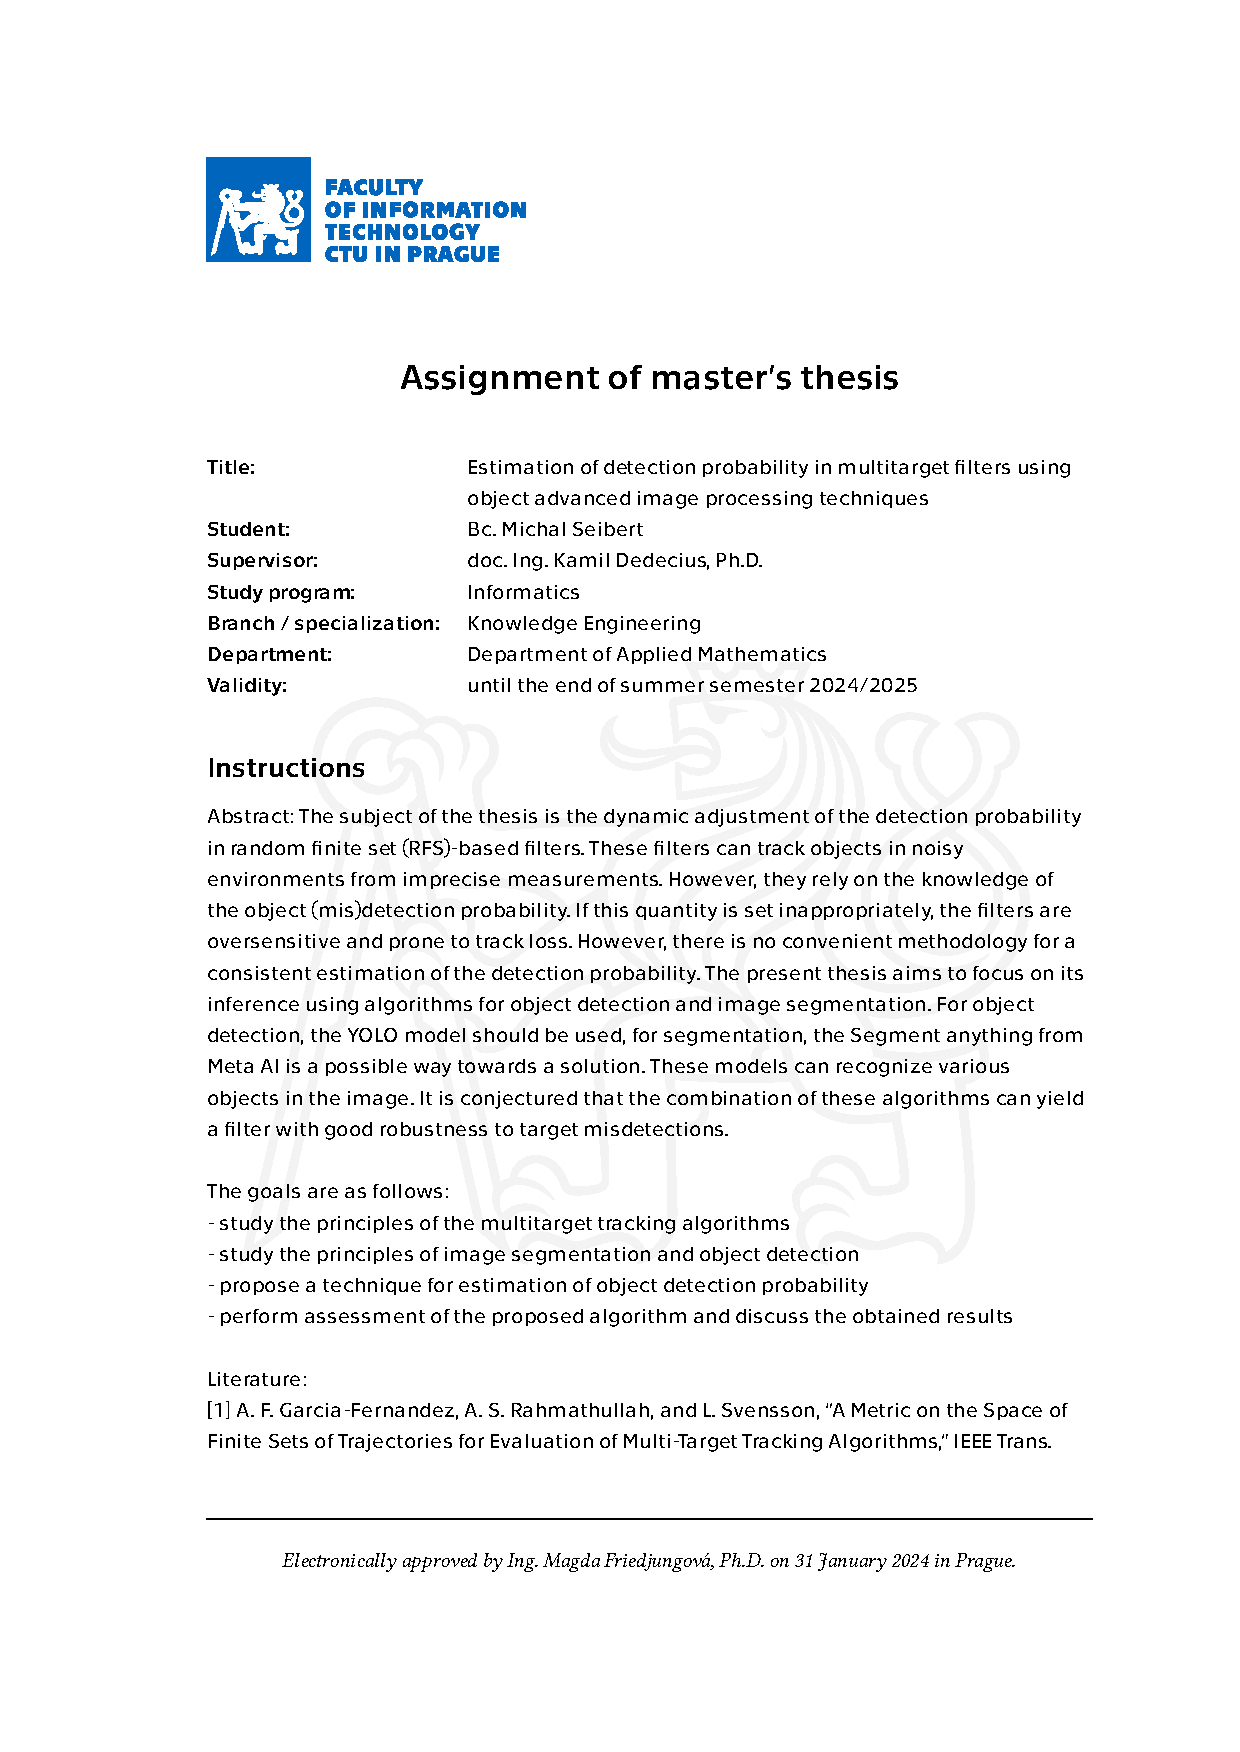
\includepdf[pages={1-}]{seibemic-assignment.pdf} % replace that file with your thesis assignment provided by study office

\thispagestyle{empty}\cleardoublepage\maketitle % do not remove these three commands

\imprintpage % do not remove this command

\tableofcontents % do not remove this command
%%%%%%%%%%%%%%%%%%%%%%
% list of other contents: figures, tables, code listings, algorithms, etc.
% add/remove commands accordingly
%%%%%%%%%%%%%%%%%%%%%%
\listoffigures % list of figures
\begingroup
\let\clearpage\relax
\listoftables % list of tables
\lstlistoflistings % list of source code listings generated by the listings package
% \listoflistings % list of source code listings generated by the minted package
\endgroup
%%%%%%%%%%%%%%%%%%%%%%
% list of other contents END
%%%%%%%%%%%%%%%%%%%%%%

%%%%%%%%%%%%%%%%%%%
% ACKNOWLEDGMENT
% FILL IN / MODIFY
% This is a place to thank people for helping you. It is common to thank your supervisor.
%%%%%%%%%%%%%%%%%%%
\begin{acknowledgmentpage}
	Chtěl bych poděkovat především sit amet, consectetuer adipiscing elit. Curabitur sagittis hendrerit ante. Class aptent taciti sociosqu ad litora torquent per conubia nostra, per inceptos hymenaeos. Cras pede libero, dapibus nec, pretium sit amet, tempor quis. Sed vel lectus. Donec odio tempus molestie, porttitor ut, iaculis quis, sem. Suspendisse sagittis ultrices augue.
\end{acknowledgmentpage} 
%%%%%%%%%%%%%%%%%%%
% ACKNOWLEDGMENT END
%%%%%%%%%%%%%%%%%%%


%%%%%%%%%%%%%%%%%%%
% DECLARATION
% FILL IN / MODIFY
%%%%%%%%%%%%%%%%%%%
% INSTRUCTIONS
% ENG: choose one of approved texts of the declaration. DO NOT CREATE YOUR OWN. Find the approved texts at https://courses.fit.cvut.cz/SFE/download/index.html#_documents (document Declaration for FT in English)
% CZE/SLO: Vyberte jedno z fakultou schvalenych prohlaseni. NEVKLADEJTE VLASTNI TEXT. Schvalena prohlaseni najdete zde: https://courses.fit.cvut.cz/SZZ/dokumenty/index.html#_dokumenty (prohlášení do ZP)
\begin{declarationpage}
FILL IN ACCORDING TO THE INSTRUCTIONS. VYPLŇTE V SOULADU S POKYNY. Lorem ipsum dolor sit amet, consectetuer adipiscing elit. Curabitur sagittis hendrerit ante. Class aptent taciti sociosqu ad litora torquent per conubia nostra, per inceptos hymenaeos. Cras pede libero, dapibus nec, pretium sit amet, tempor quis. Sed vel lectus. Donec odio tempus molestie, porttitor ut, iaculis quis, sem. Suspendisse sagittis ultrices augue. Donec ipsum massa, ullamcorper in, auctor et, scelerisque sed, est. In sem justo, commodo ut, suscipit at, pharetra vitae, orci. Pellentesque pretium lectus id turpis.

Lorem ipsum dolor sit amet, consectetuer adipiscing elit. Curabitur sagittis hendrerit ante. Class aptent taciti sociosqu ad litora torquent per conubia nostra, per inceptos hymenaeos. Cras pede libero, dapibus nec, pretium sit amet, tempor quis. Sed vel lectus. Donec odio tempus molestie, porttitor ut, iaculis quis, sem. Suspendisse sagittis ultrices augue. Donec ipsum massa, ullamcorper in, auctor et, scelerisque sed, est. In sem justo, commodo ut, suscipit at, pharetra vitae, orci. Pellentesque pretium lectus id turpis.
\end{declarationpage}
%%%%%%%%%%%%%%%%%%%
% DECLARATION END
%%%%%%%%%%%%%%%%%%%

\printabstractpage % do not remove this command

%%%%%%%%%%%%%%%%%%%
% SUMMARY
% FILL IN / MODIFY
% OR REMOVE ENTIRELY (upon agreement with your supervisor)
% (appropriate to remove in most theses)
%%%%%%%%%%%%%%%%%%%
% \begin{summarypage}
% \section*{Summary section}
% 
% \lipsum[1][1-8]
% 
% \section*{Summary section}
% 
% \lipsum[2][1-6]
% 
% \section*{Summary section}
% 
% \lipsum[3]
% 
% \section*{Summary section}
% 
% \lipsum[2]
% 
% \section*{Summary section}
% 
% \lipsum[1][1-8] Lorem lorem lorem.
% \end{summarypage}
%%%%%%%%%%%%%%%%%%%
% SUMMARY END
%%%%%%%%%%%%%%%%%%%

%%%%%%%%%%%%%%%%%%%
% ABBREVIATIONS
% FILL IN / MODIFY
% OR REMOVE ENTIRELY
% List the abbreviations in lexicography order.
%%%%%%%%%%%%%%%%%%%
\chapter{Seznam zkratek}
	
\begin{tabular}{rl}
DFA & Deterministic Finite Automaton\\
FA & Finite Automaton\\
LPS & Labelled Prüfer Sequence\\
NFA & Nondeterministic Finite Automaton\\
NPS & Numbered Prüfer Sequence\\
XML & Extensible Markup Language\\
XPath & XML Path Language\\
XSLT & eXtensible Stylesheet Language Transformations\\
W3C & World Wide Web Consortium
\end{tabular}
%%%%%%%%%%%%%%%%%%%
% ABBREVIATIONS END
%%%%%%%%%%%%%%%%%%%

\mainmatter\mainmatterinit % do not remove these two commands

%%%%%%%%%%%%%%%%%%%
% THE THESIS
% MODIFY ANYTHING BELOW THIS LINE
%%%%%%%%%%%%%%%%%%%
%\large
% Do not forget to include Introduction
%---------------------------------------------------------------
%\chapter{Introduction}
% uncomment the following line to create an unnumbered chapter
\chapter*{Introduction}\addcontentsline{toc}{chapter}{Introduction}\markboth{Introduction}{Introduction}
%---------------------------------------------------------------
\setcounter{page}{1}

% The following environment can be used as a mini-introduction for a chapter. Use that any way it pleases you (or comment it out). It can contain, for instance, a summary of the chapter. Or, there can be a quotation.
%\begin{chapterabstract}
	
%\end{chapterabstract}
%\section{Preface to multi target tracking}
Multi-target tracking (MTT), a fundamental aspect of surveillance and monitoring systems, has undergone significant advancements in recent years, transforming it into a critical field with diverse applications across various domains. 
The scope of MTT extends beyond mere tracking, encompassing tasks such as object detection, identification, and trajectory prediction. The primary goal is to maintain a comprehensive situational awareness, providing invaluable information for decision-making processes in various applications, ranging from defense and surveillance to autonomous systems and robotics.
This section provides an overview of the evolution, applications, significance, and current research focus of multi-target tracking.
            \section{Evolution and development}
The roots of MTT can be traced back to the early 20th century when radar technology emerged during World War II \cite{bar1995}. Initially developed for single-target detection, radar systems laid the groundwork for subsequent advancements in multi-target tracking. As scenarios evolved and became more complex, the need for advanced tracking capabilities grew, prompting the development of more sophisticated algorithms.

The 1970s and 1980s witnessed the emergence of basic tracking algorithms, marking the initial forays into the field. Subsequent decades saw the integration of probabilistic techniques, such as the Kalman filter \cite{kalmanFilter}, which significantly enhanced tracking accuracy. . The 2000s marked the transition to data-driven approaches, with particle filters gaining popularity due to their ability to handle non-linear and non-Gaussian tracking scenarios \cite{nonlinearParticleFilter}. However, due to the high computational complexity of particle filters, much attention is paid to data association filters such as JPDA \cite{brekke} or RFS based filters \cite{mahler}.

        \section{Applications of multi-target tracking}
The versatility of MTT is reflected in its diverse applications across various domains. In defense, MTT plays a pivotal role in monitoring and tracking multiple targets simultaneously, aiding in threat assessment, target prioritization, and distinguishing friend from foe.

The advent of autonomous systems, particularly in vehicles, has heightened the importance of MTT in predicting and tracking the movements of pedestrians, vehicles, and other obstacles. This application enhances the safety and efficiency of autonomous vehicles by providing real-time awareness of the surrounding environment \cite{milan2016}.

Surveillance systems rely on multi-target tracking for monitoring activities in crowded environments and identifying suspicious behavior

Moreover, in fields such as robotics, defense, healthcare monitoring, and wildlife conservation, multi-target tracking systems contribute significantly to enhancing situational awareness, enabling real-time decision-making, improving resource allocation efficiency, and supporting various mission-critical tasks.

%        \subsection{Research interests}
%Contemporary research in multi-target tracking is characterized by a strong emphasis on addressing %key challenges to further enhance the performance and robustness of tracking systems. Researchers %are exploring innovative approaches to improve data association accuracy, handle complex motion %patterns, mitigate effects of occlusions and clutter in the environment, optimize computational %efficiency, and enhance detection probabilities.

%State-of-the-art techniques such as probabilistic modeling for uncertainty quantification %\cite{bar1995}, optimization algorithms for track association optimization, and sensor fusion for %integrating information from multiple sources are being leveraged to push the boundaries of multi-%target tracking capabilities.

        \section{Multi target algorithms}
The field of multi-target tracking is marked by a rich and diverse landscape of algorithms, each tailored to address specific challenges inherent in tracking multiple objects. These algorithms can be broadly categorized into association-based methods and Random Finite Set (RFS) based methods, each offering unique advantages and trade-offs.

Association-based methods form a foundational category in multi-target tracking, emphasizing the linking of measurements to existing tracks or the creation of new tracks. The well-established Kalman filter and its variants, such as the Extended Kalman Filter (EKF) and Unscented Kalman Filter (UKF), fall under this category. More advanced methods considering clutter such as Probabilistic Association (PDA) filter, Joint Probabilistic Association (JPDA) filter or Multiple Hypothesis Tracker (MHT) filter are another examples of filters from this category.

In contrast to association-based methods, Random Finite Set (RFS) based methods provide a probabilistic framework to model multiple target states simultaneously. These methods operate on sets of possible target states, allowing for a more comprehensive representation of uncertainty and variability in tracking scenarios. The Probability Hypothesis Density (PHD) filter, Cardinalized Probability Hypothesis Density (CPHD) or Poisson multi-Bernoulli mixture (PMBM) filter are prominent examples of an RFS-based approach.

        \section{Research interests}
Contemporary research in multi-target tracking is characterized by a strong emphasis on addressing key challenges to further enhance the performance and robustness of tracking systems. Current research focus deald with problems such as:
\begin{itemize}
    \item \textbf{Data Association in complex environment:}  Handling scenarios with high target density, occlusions, and clutter remains a complex issue. Robust methods for accurate and efficient data association in crowded and dynamic environments are still actively researched.
    \item \textbf{Handling non-linear and non-gaussian dynamics:}  Real-world scenarios often exhibit non-linear and non-Gaussian characteristics. Improving tracking algorithms to effectively handle these complexities, possibly through the integration of advanced probabilistic models is an ongoing area of research.
    \item \textbf{Real-time processing and computational efficiency:} Many MTT algorithms, especially those with high computational demands, face challenges in meeting real-time processing requirements. Efficient algorithms that strike a balance between computational complexity and tracking accuracy are continuously sought.
    \item \textbf{Sensor fusion and heterogeneous data integration:} Integrating information from various sensors, each with its own characteristics and limitations, is an ongoing challenge. Developing robust methods for sensor fusion to improve tracking accuracy and reliability is an active research area.
    \item \textbf{Handling variability in target behavior:} Targets in real-world scenarios may exhibit diverse and unpredictable behaviors. Adapting tracking algorithms to handle varying target speeds, accelerations, and maneuvers remains an unsolved problem.
    \item \textbf{Online learning and adaptive algorithms:} Designing algorithms that can adapt and learn online as they encounter new scenarios or dynamic changes in the environment is a topic of interest. Adaptive tracking systems that can continuously improve their performance without extensive retraining are sought after.
\end{itemize}
%%%%%%%%%%%%%%%%%%%%%
% Převzato z článku %
%%%%%%%%%%%%%%%%%%%%%
The probabilistic formulation of the RFS-based filters and the inherent Bayesian processing of available information allow to accommodate the uncertainty arising from the presence of false detections, missed detections, and data association ambiguities. Nevertheless, a fundamental challenge persists: The performance of the filters is highly sensitive to the accurate setting of the target detection probability. This quantity, representing the likelihood of correctly identifying and associating observations with actual targets, is a critical parameter. It has a substantial impact on the Bayesian updating of the prior information.
However, in real-world scenarios, the sensor performance is susceptible to various environmental conditions. Adverse weather, occlusions, or just the nature of the current scenario can lead to variations in detection probabilities. A mismatch between assumed and actual detection probabilities can result in a suboptimal tracking performance, leading to missed detections, false alarms, or inaccurate target state estimates \cite{Hendeby2014Gaussian}.

The RFS-based formulation of the PHD or (P)MBM filters naturally takes the uncertainty about the detection probability into account \cite{Hendeby2014Gaussian}. The update formulae involve it as a function of the target state. In the figurative sense, this allows to model it as a function of the spatial and temporal properties of the environment.
Still, two difficulties arise. First, the (Gaussian) filters are analytically tractable only if the detection probabilities are scalar numbers. Second, the nature of the detection probabilities differs from scenario to scenario. 

In general, several methods have been proposed to deal with unknown detection probabilities. A Gaussian-beta modeling of a slowly-varying detection profile in the Cardinalized PHD filter is reported in \cite{Mahler2011cphd}; its alternative for MBM filters follows in \cite{Vo2013Robust}, and for PMBM filter in \cite{Kong2021Robust}. In \cite{Li2018PHD}, the authors propose to overcome some deficiencies in the CPHD filter \cite{Mahler2011cphd} by different clutter/detection probability models. Another variant was recently proposed in \cite{wei2023BGMPHD}. A track-state augmentation with an amplitude offset-based prediction of the detection probability appeared in \cite{Hanusa2013Track}, however, this method suffers difficulties in multistatic fields. An automatic identification system-based sensor performance assessment for clutter-free environments is developed in \cite{Horn2013Near}. A recent paper \cite{Wei2022Trajectory} deals with the unknown detection profile in the trajectory PHD/CPHD filters. There, the algorithm learns from the history of the unknown target detection probability.

This thesis focuses on tracking targets in video data. This allows to avoid the generic solutions and focus on the peculiarities associated with this specific data type. In particular, advantage of YOLO (You Only Look Once) is taken, offering high-performance real-time object detection with high accuracy and efficiency \cite{yanYolo2023}. Its ability to simultaneously predict multiple bounding boxes and class probabilities within an image is used, providing a streamlined and efficient approach to object detection. However, YOLO-based multi-target tracking systems can still be compromised under conditions such as adverse weather, low lighting, or scenarios with occlusions. Sensors may encounter difficulties in accurately detecting and localizing targets, leading to gaps or errors in the tracking process.

        \section{Structure}
The structure of this thesis is as follows:
\begin{description}
\item[Chapter 1] 

\item[Chapter 2]
\item[Chapter 3] 

\item[Chapter 4] 
\end{description}

%
%\begin{definition}[Optional label]
%definition
%\end{definition}

%\begin{example}
%example
%\end{example}

%\begin{theorem}
%theorem
%\end{theorem}

%\begin{proof}
%proof
%\end{proof}

%\begin{corollary}
%corollary
%\end{corollary}

%\begin{proposition}
%proposition
%\end{proposition}

%\begin{note}
%note
%\end{note}

%\begin{remark}
%remark
%\end{remark}

%\begin{lemma}
%lemma
%\end{lemma}


 % include `text.tex' from `text/' subdirectory
\chapter{Thesis establishment}
Multi-target tracking (MTT), a fundamental aspect of surveillance and monitoring systems, has undergone significant advancements in recent years, transforming it into a critical field with diverse applications across various domains.
The scope of MTT extends beyond mere tracking, encompassing tasks such as object detection, identification, and trajectory prediction. The primary goal is to maintain a comprehensive situational awareness, providing invaluable information for decision-making processes in various applications, ranging from defense and surveillance to autonomous systems and robotics.
This section provides an overview of the evolution, applications, significance, and current research focus of multi-target tracking.
\section{Evolution and development}
The roots of MTT can be traced back to the early 20th century when radar technology emerged during World War II \cite{bar1995}. Initially developed for single-target detection, radar systems laid the groundwork for subsequent advancements in multi-target tracking. As scenarios evolved and became more complex, the need for advanced tracking capabilities grew, prompting the development of more sophisticated algorithms.

The 1970s and 1980s witnessed the emergence of basic tracking algorithms, marking the initial forays into the field. Subsequent decades saw the integration of probabilistic techniques, such as the Kalman filter \cite{kalmanFilter}, which significantly enhanced tracking accuracy. . The 2000s marked the transition to data-driven approaches, with particle filters gaining popularity due to their ability to handle non-linear and non-Gaussian tracking scenarios \cite{nonlinearParticleFilter}. However, due to the high computational complexity of particle filters, much attention is paid to data association filters such as JPDA \cite{brekke} or RFS based filters \cite{mahler}.

\section{Applications of multi-target tracking}
The versatility of MTT is reflected in its diverse applications across various domains. In defense, MTT plays a pivotal role in monitoring and tracking multiple targets simultaneously, aiding in threat assessment, target prioritization, and distinguishing friend from foe.

The advent of autonomous systems, particularly in vehicles, has heightened the importance of MTT in predicting and tracking the movements of pedestrians, vehicles, and other obstacles. This application enhances the safety and efficiency of autonomous vehicles by providing real-time awareness of the surrounding environment \cite{milan2016}.

Surveillance systems rely on multi-target tracking for monitoring activities in crowded environments and identifying suspicious behavior

Moreover, in fields such as robotics, defense, healthcare monitoring, and wildlife conservation, multi-target tracking systems contribute significantly to enhancing situational awareness, enabling real-time decision-making, improving resource allocation efficiency, and supporting various mission-critical tasks.

%        \subsection{Research interests}
%Contemporary research in multi-target tracking is characterized by a strong emphasis on addressing %key challenges to further enhance the performance and robustness of tracking systems. Researchers %are exploring innovative approaches to improve data association accuracy, handle complex motion %patterns, mitigate effects of occlusions and clutter in the environment, optimize computational %efficiency, and enhance detection probabilities.

%State-of-the-art techniques such as probabilistic modeling for uncertainty quantification %\cite{bar1995}, optimization algorithms for track association optimization, and sensor fusion for %integrating information from multiple sources are being leveraged to push the boundaries of multi-%target tracking capabilities.

\section{Multi target algorithms}
The field of multi-target tracking is marked by a rich and diverse landscape of algorithms, each tailored to address specific challenges inherent in tracking multiple objects. These algorithms can be broadly categorized into association-based methods and Random Finite Set (RFS) based methods, each offering unique advantages and trade-offs.

Association-based methods form a foundational category in multi-target tracking, emphasizing the linking of measurements to existing tracks or the creation of new tracks. The well-established Kalman filter and its variants, such as the Extended Kalman Filter (EKF) and Unscented Kalman Filter (UKF), fall under this category. More advanced methods considering clutter such as Probabilistic Association (PDA) filter, Joint Probabilistic Association (JPDA) filter or Multiple Hypothesis Tracker (MHT) filter are another examples of filters from this category.

In contrast to association-based methods, Random Finite Set (RFS) based methods provide a probabilistic framework to model multiple target states simultaneously. These methods operate on sets of possible target states, allowing for a more comprehensive representation of uncertainty and variability in tracking scenarios. The Probability Hypothesis Density (PHD) filter, Cardinalized Probability Hypothesis Density (CPHD) or Poisson multi-Bernoulli mixture (PMBM) filter are prominent examples of an RFS-based approach.

\section{Research interests}
Contemporary research in multi-target tracking is characterized by a strong emphasis on addressing key challenges to further enhance the performance and robustness of tracking systems. Current research focus deald with problems such as:
\begin{itemize}
  \item \textbf{Data Association in complex environment:}  Handling scenarios with high target density, occlusions, and clutter remains a complex issue. Robust methods for accurate and efficient data association in crowded and dynamic environments are still actively researched.
  \item \textbf{Handling non-linear and non-gaussian dynamics:}  Real-world scenarios often exhibit non-linear and non-Gaussian characteristics. Improving tracking algorithms to effectively handle these complexities, possibly through the integration of advanced probabilistic models is an ongoing area of research.
  \item \textbf{Real-time processing and computational efficiency:} Many MTT algorithms, especially those with high computational demands, face challenges in meeting real-time processing requirements. Efficient algorithms that strike a balance between computational complexity and tracking accuracy are continuously sought.
  \item \textbf{Sensor fusion and heterogeneous data integration:} Integrating information from various sensors, each with its own characteristics and limitations, is an ongoing challenge. Developing robust methods for sensor fusion to improve tracking accuracy and reliability is an active research area.
  \item \textbf{Handling variability in target behavior:} Targets in real-world scenarios may exhibit diverse and unpredictable behaviors. Adapting tracking algorithms to handle varying target speeds, accelerations, and maneuvers remains an unsolved problem.
  \item \textbf{Online learning and adaptive algorithms:} Designing algorithms that can adapt and learn online as they encounter new scenarios or dynamic changes in the environment is a topic of interest. Adaptive tracking systems that can continuously improve their performance without extensive retraining are sought after.
\end{itemize}
%%%%%%%%%%%%%%%%%%%%%
% Převzato z článku %
%%%%%%%%%%%%%%%%%%%%%
The probabilistic formulation of the RFS-based filters and the inherent Bayesian processing of available information allow to accommodate the uncertainty arising from the presence of false detections, missed detections, and data association ambiguities. Nevertheless, a fundamental challenge persists: The performance of the filters is highly sensitive to the accurate setting of the target detection probability. This quantity, representing the likelihood of correctly identifying and associating observations with actual targets, is a critical parameter. It has a substantial impact on the Bayesian updating of the prior information.
However, in real-world scenarios, the sensor performance is susceptible to various environmental conditions. Adverse weather, occlusions, or just the nature of the current scenario can lead to variations in detection probabilities. A mismatch between assumed and actual detection probabilities can result in a suboptimal tracking performance, leading to missed detections, false alarms, or inaccurate target state estimates \cite{Hendeby2014Gaussian}.

The RFS-based formulation of the PHD or (P)MBM filters naturally takes the uncertainty about the detection probability into account \cite{Hendeby2014Gaussian}. The update formulae involve it as a function of the target state. In the figurative sense, this allows to model it as a function of the spatial and temporal properties of the environment.
Still, two difficulties arise. First, the (Gaussian) filters are analytically tractable only if the detection probabilities are scalar numbers. Second, the nature of the detection probabilities differs from scenario to scenario.

In general, several methods have been proposed to deal with unknown detection probabilities. A Gaussian-beta modeling of a slowly-varying detection profile in the Cardinalized PHD filter is reported in \cite{Mahler2011cphd}; its alternative for MBM filters follows in \cite{Vo2013Robust}, and for PMBM filter in \cite{Kong2021Robust}. In \cite{Li2018PHD}, the authors propose to overcome some deficiencies in the CPHD filter \cite{Mahler2011cphd} by different clutter/detection probability models. Another variant was recently proposed in \cite{wei2023BGMPHD}. A track-state augmentation with an amplitude offset-based prediction of the detection probability appeared in \cite{Hanusa2013Track}, however, this method suffers difficulties in multistatic fields. An automatic identification system-based sensor performance assessment for clutter-free environments is developed in \cite{Horn2013Near}. A recent paper \cite{Wei2022Trajectory} deals with the unknown detection profile in the trajectory PHD/CPHD filters. There, the algorithm learns from the history of the unknown target detection probability.

This thesis focuses on tracking targets in video data. This allows to avoid the generic solutions and focus on the peculiarities associated with this specific data type. In particular, advantage of YOLO (You Only Look Once) is taken, offering high-performance real-time object detection with high accuracy and efficiency \cite{yanYolo2023}. Its ability to simultaneously predict multiple bounding boxes and class probabilities within an image is used, providing a streamlined and efficient approach to object detection. However, YOLO-based multi-target tracking systems can still be compromised under conditions such as adverse weather, low lighting, or scenarios with occlusions. Sensors may encounter difficulties in accurately detecting and localizing targets, leading to gaps or errors in the tracking process.

\section{Structure}
The structure of this thesis is as follows:
\begin{description}
  \item[Chapter 1]

  \item[Chapter 2]
  \item[Chapter 3]

  \item[Chapter 4]
\end{description}
\chapter{Theoretical Background}
Multi-target tracking relies heavily on mathematical concepts from the probability theory, statistics, and linear algebra to model and infer the state of multiple objects over time. The key mathematical concepts involved in MTT include Bayesian inference, which provides a framework for updating estimates based on observed evidence, and the use of probabilistic models such as the Gaussian distribution and its extensions, such as Gaussian mixture models. In addition, MTT commonly employs state space models to represent the dynamics of object motion, with popular models including the constant velocity and constant acceleration models. These models are integrated into Bayesian filters, such as the Kalman filter, which recursively estimates the state of a target given by noisy measurements.
%\section{Foundations of probability theory}
%\section{Probability distributions}
%    \subsection{Bernoulli distribution}
%    \subsection{Uniform distribution}
%    \subsection{Poisson distribution}
%    \subsection{Gaussian (Normal) distribution}
    \section{Bayesian inference}
Bayesian inference stands as a foundational pillar within the realm of a probabilistic reasoning, offering a fundamental methodology for systematically updating beliefs in response to observed evidence. A fundamental theorem in probability theory, the Bayes' rule, is rooted in the Bayesian inference. It formalizes the process of revising prior beliefs in light of new data. The essence of Bayesian inference transcends mere statistical calculations; it embodies a philosophical stance towards uncertainty, emphasizing the incorporation of prior knowledge and the iterative refinement of beliefs through the assimilation of empirical observations. Within the context of multi-target tracking, Bayesian inference plays a paramount role, providing a principled framework for joining information from disparate sources, such as sensor measurements, historical data, and domain expertise. By embracing Bayesian principles, MTT algorithms gain the capacity to model and quantify uncertainty inherent in tracking scenarios, thereby fostering robustness and adaptability in the face of dynamic and complex environments. Moreover, Bayesian inference empowers MTT systems to exploit contextual cues and domain-specific knowledge, enhancing their ability to discern meaningful patterns among noise and uncertainty. Due to the Bayesian inference, MTT researchers and practitioners are equipped with a powerful tool for navigating the intricacies of multi-target tracking, facilitating informed decision-making and advancing the frontier of robust systems. Thus, Bayesian inference emerges not merely as a mathematical construct, but as a guiding philosophy underpinning the quest for understanding and reasoning in the face of uncertainty.
    \section{Bayes' rule}
Bayes' rule, a cornerstone of Bayesian inference, embodies a fundamental principle in probability theory that underpins the systematic revision of beliefs in the face of new evidence. Mathematically expressed as a simple formula, Bayes' rule encapsulates the process of updating prior probabilities based on observed data, thereby yielding posterior probabilities that reflect the incorporation of new information. At its basis, the Bayes' rule provides a formal mechanism for quantifying the impact of new evidence on the likelihood of various hypotheses or states of nature. The rule states that the posterior probability of a hypothesis given observed data is proportional to the product of the likelihood of the data given the hypothesis and the prior probability of the hypothesis, divided by the marginal likelihood of the data. In essence, Bayes' rule facilitates a principled approach to inference, allowing practitioners to integrate prior knowledge with empirical observations to arrive to more informed and reliable conclusions. In the context of multi-target tracking, Bayes' rule serves as the base upon which the tracking algorithms are built, enabling the continuous refinement of estimates about the state of multiple targets based on sensor measurements and historical data. By adhering to the principles of Bayes' rule, MTT systems can effectively navigate the inherent uncertainty and complexity of tracking scenarios, thereby enhancing their robustness and accuracy.
    \begin{definition}[Conditional distribution]
    Let $X$ and $Y$ be jointly continuous random variables, $f_Y$ continuous at $y$ and $f_Y(y) > 0$. Then the conditional distribution function of $X$, given condition ${Y=y}$ is defined by
    \end{definition}
    \begin{align}
        F_{X|Y}(x|y) &:= \lim_{\epsilon\to0} \textbf{P}\{X\leq x | Y \in (y, y + \epsilon)\} = \frac{\partial F(x,y) /
        \partial y}{f_Y(y)}.\label{eq:conditional_distribution}
    \end{align}
    Differentiating this, the conditional density function of $X$, given the condition ${Y = y}$, is
    \begin{align}
        f_{X|Y}(x|y) &:= \frac{ \frac{\partial^2 F(x,y)}{\partial x \partial y}}{f_Y(y)} = \frac{f(x,y)}{f_Y(y)}. \label{eq:conditional_distribution2}
    \end{align}
    Naturally, fixing $y$, $F_{X|Y}(\cdot|y)$ and $f_{X|Y}(\cdot|y)$ are proper distribution and density functions, respectively. It is also clear that $X$ and $Y$ are independent if and only if $F_{X|Y}(x|y) = F_X(x)$ and $f_{X|Y}(x|y) = f_X(x)$ for all $x$ and $y$ for which these quantities are defined.

    \begin{definition}[Bayes' theorem]
    Let $x$ and $x$ be random variables with densities $f(y|x)$ and $f(x)$. Then Bayes' theorem is defined as
    \end{definition}
    \begin{align}
        f(x|y) &= \frac{f(y|x) f(x)}{f(y)}, \quad f(y) > 0,\label{eq:bayes_rule}
    \end{align}
where 
    \begin{itemize}
        \item $f(x|y) $ is the conditional posterior density of $x$,
        \item $f(x)$ is prior density,
        \item  $f(y|x)$ is likelihood and $f(x)$ is marginal density of $X$, also called $evidence$, and is given by 
            \begin{align}
            f(y) = \int f(x,y) \partial x \label{eq:marginal_density}.
            \end{align}
    \end{itemize}
    
Combining Equations \eqref{eq:conditional_distribution}, \eqref{eq:conditional_distribution2} and \eqref{eq:marginal_density} to Formula \eqref{eq:bayes_rule} we get complete formula for Bayes' theorem
    \begin{align}
        f(x|y) &= \frac{f(y|x) f(x)}{f(y)} = \frac{f(y|x) f(x)}{\int f(y|x) f(x) \partial x}. \label{eq:bayes_full}
    \end{align}
The denominator is the normalizing constant independent of $x$, often only proportionality is used
    \begin{align}
        f(x|y) &\propto f(y|x)f(x).
    \end{align}











    
    \section{Multivariate Gaussian distribution}
In the realm of multi-target tracking, various probability distributions are employed to model the uncertainty
associated with target states and measurements. However, among these distributions, the multivariate Gaussian distribution holds a preeminent position due to its versatility, mathematical tractability, and empirical relevance. While other distributions may capture specific aspects of target behavior or measurement noise, the Gaussian distribution emerges as the cornerstone of MTT due to its ability to characterize complex probability distributions in multi-dimensional spaces. As a result, the common assumption among MTT filters is that the targets follow linear Gaussian dynamics and measuremets models, as in \cite{bar1995}, \cite{GarciaPMBM2018}, or \cite{VoMaPHD2006}. The Gaussian distribution finds ubiquitous application across various components of tracking algorithms, including
\begin{itemize}
    \item \textbf{State representation:} Gaussian distributions are used to model the probability distributions of target states, allowing for efficient representation and propagation of uncertainty over time.
    \item \textbf{Measurement model:} Gaussian distributions are employed to model the likelihood of sensor measurements given the true target state, facilitating the incorporation of sensor data into the tracking process.
    \item \textbf{Filtering algorithms:} Gaussian-based filters leverage the Gaussian assumption to derive recursive estimation algorithms for tracking multiple targets with optimal efficiency and accuracy.
    \item \textbf{Data association:} Gaussian mixture models (GMMs), which represent mixtures of Gaussian distributions, are utilized for probabilistic data association in MTT, enabling robust handling of measurement uncertainty and target ambiguity.
\end{itemize}
\begin{note}
The multivariate Gaussian distribution is a generalization of the univariate Gaussian distribution, but instead of a scalar mean and variance, there is a mean vector and a covariance matrix, that describe correlations between variables. The distribution of a $k-$dimensional random vector $\mathbf{X} = (X_1,\dots,X_k)^T$ and can be written in the notation
\[\mathbf{X} \thicksim \mathcal{N}(\mathbf{\mu}, \mathbf{\Sigma}),\]
with
$k-$dimensional mean vector
$\mathbf{\mu} = \mathsf{E}[\mathbf{X}] = (\mathsf{E}[X_1], \mathsf{E}[X_1], \dots, \mathsf{E}[X_k])^T$
and
$k\times k$ positive semi-definite covariance matrix $\Sigma$, with elements
\begin{align}
    \mathbf{\Sigma}_{ij} &= \mathsf{E}[(X_i - \mu_i)(X_j - \mu_j)] = Cov[X_i, X_j].
\end{align}

\end{note}
The probability density function (PDF) is given by formula
\begin{align}
    \mathcal{N}(\mathbf{x};\mathbf{\mu},\mathbf{\Sigma}) &= \frac{1}{\sqrt{(2\pi)^k |\mathbf{\Sigma}|}}\exp \left(-\frac{1}{2}(\mathbf{x}-\mathbf{\mu})^T\mathbf{\Sigma}^{-1}(\mathbf{x}-\mathbf{\mu}) \right),
\end{align}
where $k$ is the length of the vector $\mathbf{x}$ and $|\cdot|$ denotes the determinant of a matrix. It should be noted that the exponent is known as Mahalanobis distance.
\begin{definition}[Mahalanobis distance]
    For vectors $x$ and $y$ and a positive semi-definite matrix $S$, the Mahalanobis distance between two objects is defined as
    \begin{align}
        d(\mathbf{x},\mathbf{y}) = \sqrt{(\mathbf{x}-\mathbf{y})^T S^{-1} (\mathbf{x}-\mathbf{y})}
    \end{align}
\end{definition}
The Mahalanobis distance (MD) is the distance between two points in a multivariate space and, unlike Eucledian distance, it measures distances even between the correlated points for multiple variables.

Target tracking filters regularly use conditional probabilities and joint distributions, especially Gaussian. 
\begin{theorem}[Conditional joint Gaussian distribution]
Let $\mathbf{x}$ and $\mathbf{y}$ are Gaussian random variables with distributions $ \mathcal{N}(\mathbf{x};\mathbf{\mu_x},\mathbf{\Sigma_{xx}})$ and $ \mathcal{N}(\mathbf{y};\mathbf{\mu_y},\mathbf{\Sigma_{y}})$, respectively. Let their joint probability is given by
    \begin{align}
        p(\mathbf{x}, \mathbf{y}) &= \mathcal{N}\left(
        \begin{bmatrix}
           \mathbf{x}\\
           \mathbf{y}
        \end{bmatrix};
        \begin{bmatrix}
           \mathbf{\mu_x}\\
           \mathbf{\mu_y}
        \end{bmatrix},
        \begin{bmatrix}
           \mathbf{\Sigma_{xx}} & \mathbf{\Sigma_{xy}}\\
           \mathbf{\Sigma_{xy}} & \mathbf{\Sigma_{yy}}
        \end{bmatrix}
       \right).
    \end{align}
Then the conditional distribution of $\mathbf{x}$ given by $\mathbf{y}$ is defined as
    \begin{align}
         p(\mathbf{x}|\mathbf{y}) &= \mathcal{N}(\mathbf{x};\mathbf{\mu_{x|y}},\mathbf{\Sigma_{x|y}}),
    \end{align}
where 
    \begin{align}
        \mathbf{\mu_{x|y}} &= \mathbf{\mu_{x}} + \mathbf{\Sigma_{xy}} 
        \mathbf{\Sigma_{yy}}^{-1}(\mathbf{y} - \mathbf{\mu_{y}}),\\
        \mathbf{\Sigma_{x|y}} &= \mathbf{\Sigma_{xx}} - \mathbf{\Sigma_{xy}}
        \mathbf{\Sigma_{yy}^{-1}}\mathbf{\Sigma_{xy}^T}.
    \end{align}
\end{theorem}

Examples of a multivariate Gaussian distribution are shown in Figure \ref{fig:mvnplot} and marginal distributions for
multivariate Gaussian distribution can be found in Figure \ref{fig:gaussWithMarginals}.
\begin{figure}[htbp]
    \centering
    \begin{subfigure}[b]{0.45\textwidth}
        \centering
        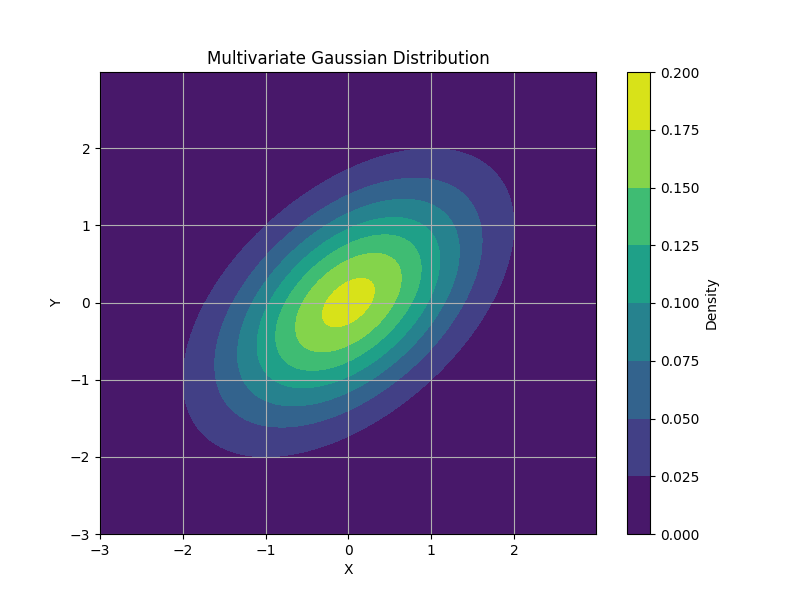
\includegraphics[width=\textwidth]{text/chapter_01/imgs/mvn_contour}
        \caption{Example of multivariate Gaussian distribution - contour plot.}
        \label{fig:mvn_contour}
    \end{subfigure}
    \hfill
    \begin{subfigure}[b]{0.45\textwidth}
        \centering
        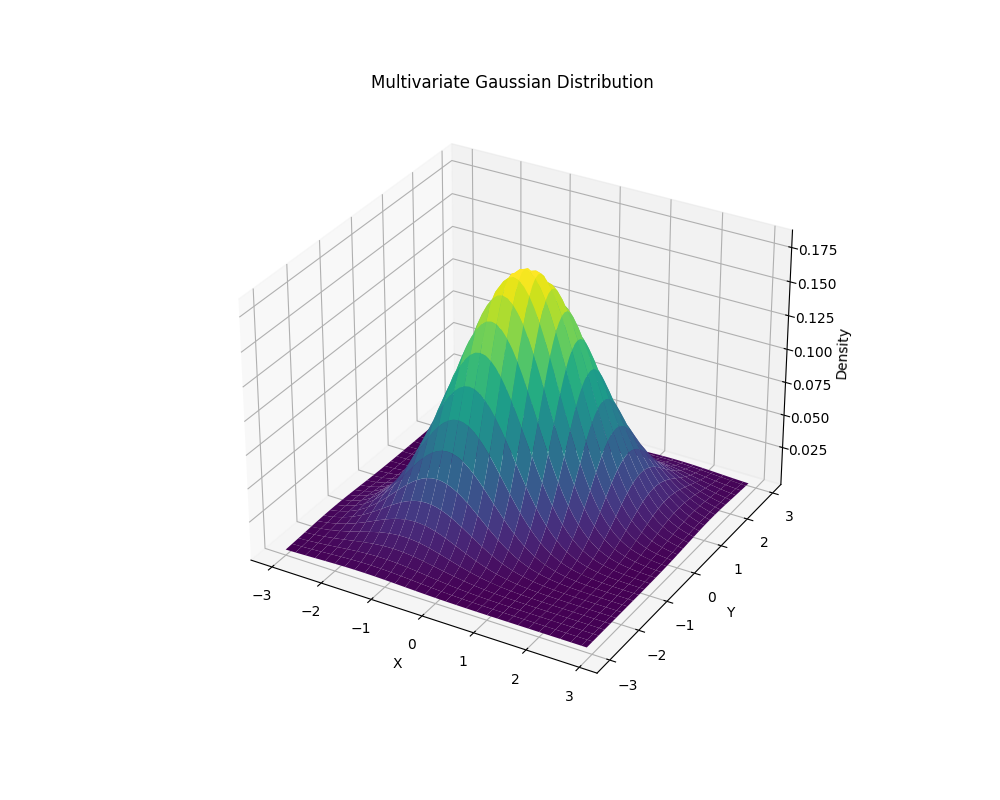
\includegraphics[width=\textwidth]{text/chapter_01/imgs/mvn_3d}
        \caption{Example of multivariate Gaussian distribution - 3D plot.}
        \label{fig:mvn_3d}
    \end{subfigure}
    \caption{Examples of plots of multivariate Gaussian distribution.}
    \label{fig:mvnplot}
\end{figure}

\begin{figure}[htbp]
    \centering
    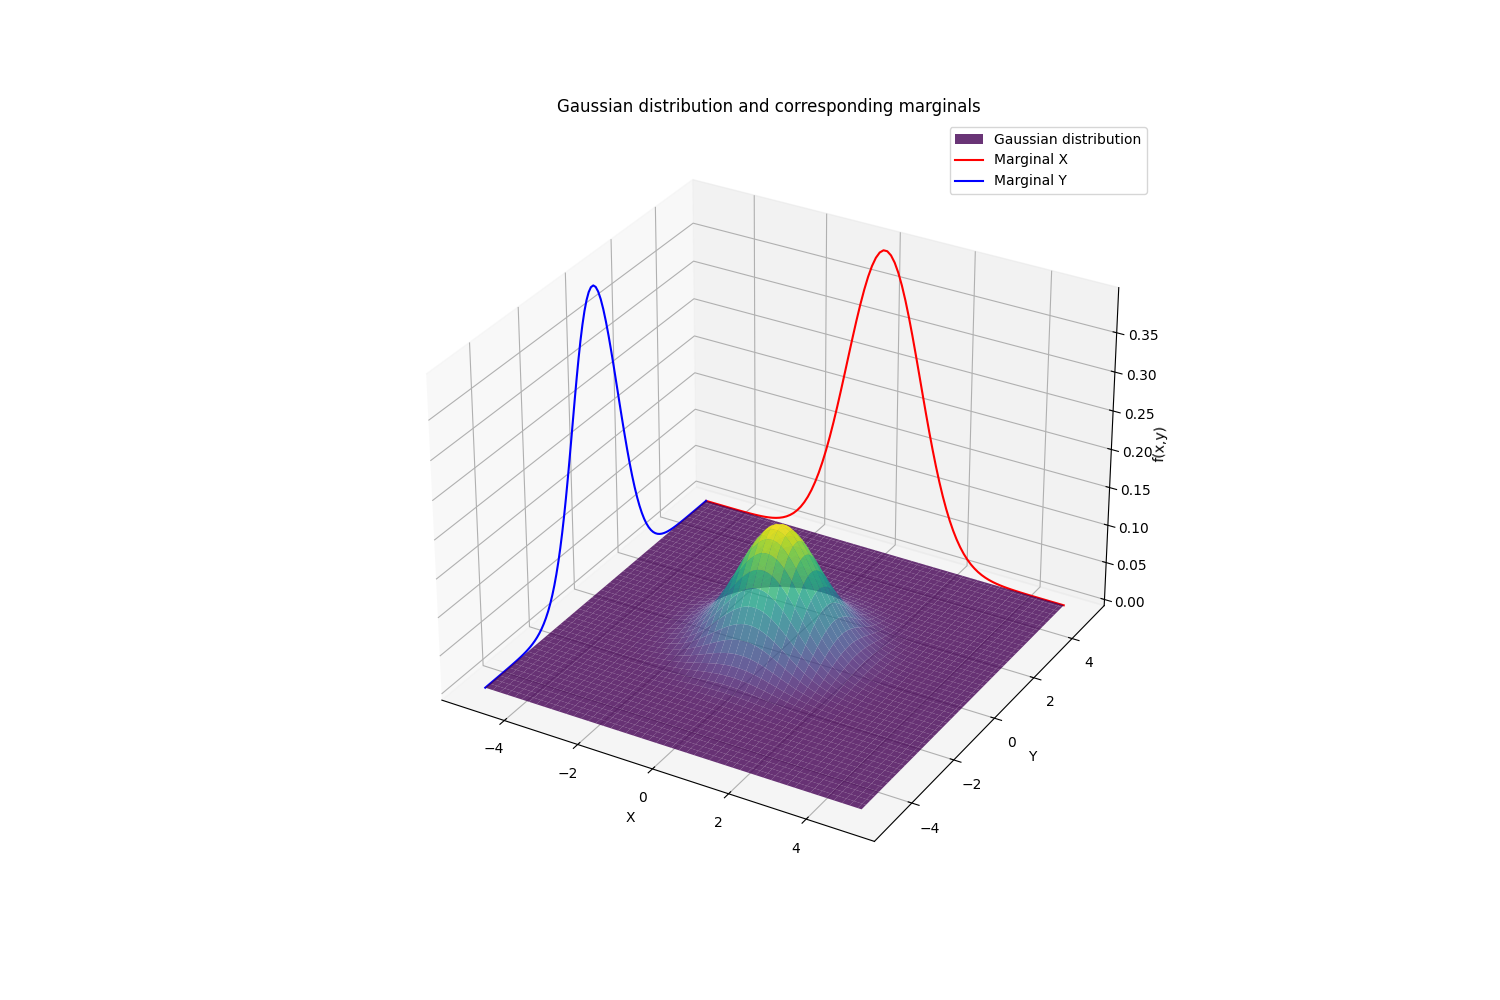
\includegraphics[width=1\textwidth]{text/chapter_01/imgs/gauss_with_marginals}
    \caption{Gaussian distribution with corresponding marginals.}
    \label{fig:gaussWithMarginals}
\end{figure}
    \section{Gaussian mixture}
%A Bayesian Gaussian mixture model is commonly extended to fit a vector of unknown parameters, or multivariate normal
%distributions. In a multivariate distribution, a vector of parameters (such as several observations of a signal) is modeled using a Gaussian mixture model prior distribution on the vector of estimates given by
Gaussian Mixture Models offer a flexible and powerful framework for representing complex probability distributions by combining multiple Gaussian components. In the Gaussian mixture model, a vector of parameters (e.g., observations of a signal) is modeled using a mixture distribution comprising several Gaussian components.
    \begin{align}
        p(\Theta) = \sum_{i=1}^k w_i \mathcal{N}(\mathbf{\mu}_i, \mathbf{\Sigma}_i),
    \end{align}
where the $i^{th}$ vector component is characterized by Gaussian distributions with weights $w_i$, means $\mathbf{\mu}
_i$ and covariance matrices $\mathbf{\Sigma}_i$. These parameters are encapsulated to the parameter $\Theta$ in $p(\cdot)$.

%In multi-target tracking, we are often dealing with linear Gaussian models, thus the posterior density is
%represented as a mixture of one or many Gaussian components. The pdf of Gaussian mixture distribution is simple sum of every Gaussian component, so the formula is as follows:
In the context of multi-target tracking, Gaussian mixture models find utility in capturing the complex nature of target states and measurements. MTT often involves dealing with linear Gaussian models, where the posterior density is represented as a mixture of one or more Gaussian components. This representation enables MTT algorithms to probabilistically model the uncertainties associated with target dynamics, sensor measurements, and data association.

The probability density function (pdf) of a Gaussian mixture distribution is a simple sum of each Gaussian component, expressed as
    \begin{align}
        p(x) &= \sum_{i=1}^k w_i\mathcal{N}(\mathbf{x};\mathbf{\mu_i}, \mathbf{\Sigma_i}),
    \end{align}
where $k$ is the number of Gaussian component, $w_i>0$ is the weight of $i^{th}$ component and $\sum_{i=1}^k w_i = 1$.

In MTT, Gaussian mixture models are particularly useful for tasks such as data association, where they probabilistically assign measurements to existing tracks or create new tracks based on the likelihood of observations given the target states. By modeling complex distributions of target states and measurements, Gaussian mixture models enable the MTT algorithms to handle uncertainties and ambiguities inherent in real-world tracking scenarios, including occlusions, clutter, and target interactions.

Examples of multivariate Gaussian mixture distribution are shown in Figure \ref{fig:mvn_mixture_plot}. Gaussian mixture distribution with marginal distribution for each dimension in Figure \ref{fig:gaussMixWithMarginals}.
\begin{figure}[htbp]
    \centering
    \begin{subfigure}[b]{0.45\textwidth}
        \centering
        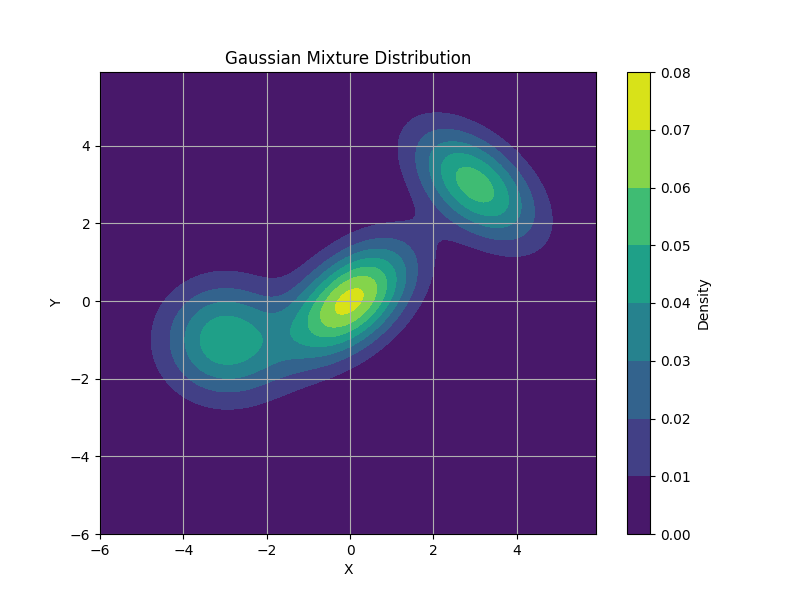
\includegraphics[width=\textwidth]{text/chapter_01/imgs/mvn_mixture_contour}
        \caption{Example of multivariate Gaussian mixture distribution - contour plot.}
        \label{fig:mvn_mixture_contour}
    \end{subfigure}
    \hfill
    \begin{subfigure}[b]{0.45\textwidth}
        \centering
        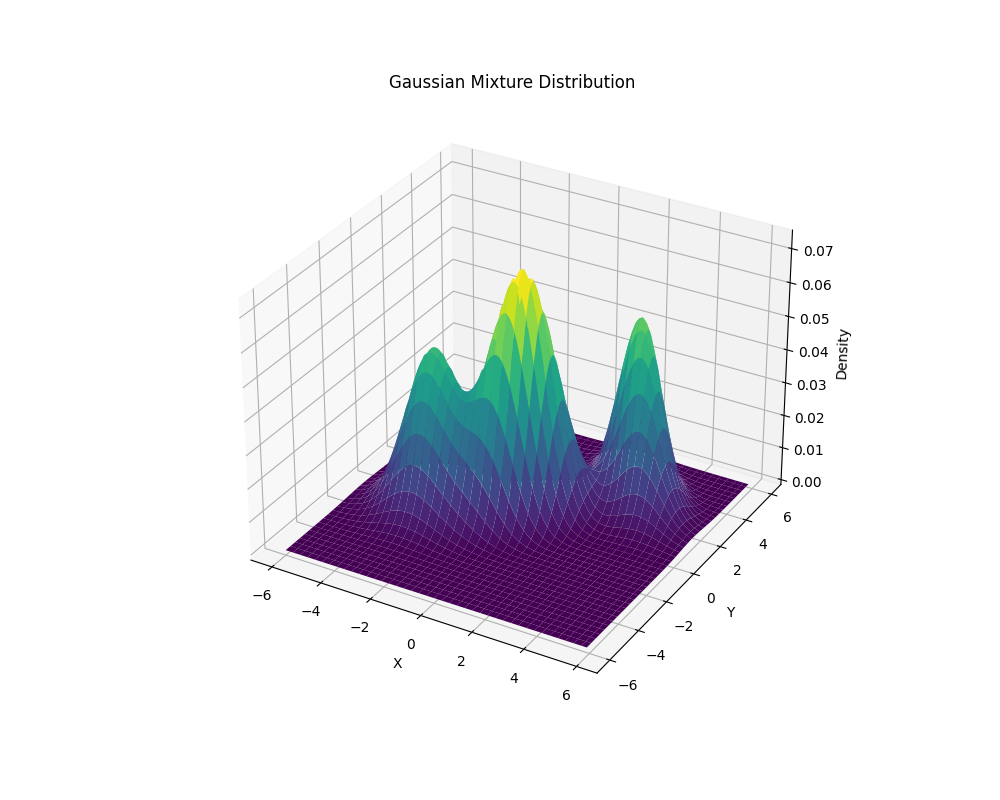
\includegraphics[width=\textwidth]{text/chapter_01/imgs/mvn_mixture_3d}
        \caption{Example of multivariate Gaussian mixture distribution - 3D plot.}
        \label{fig:mvn_mixture_3d}
    \end{subfigure}
    \caption{Examples of plots of multivariate Gaussian mixture distribution. There are three components in figures with means $\{[0, 0], [3, 3], [-3, -1]\}$. Note that the density of peaks is very low, because the sum has to be equal $1$.}
    \label{fig:mvn_mixture_plot}
\end{figure}

\begin{figure}[htbp]
    \centering
    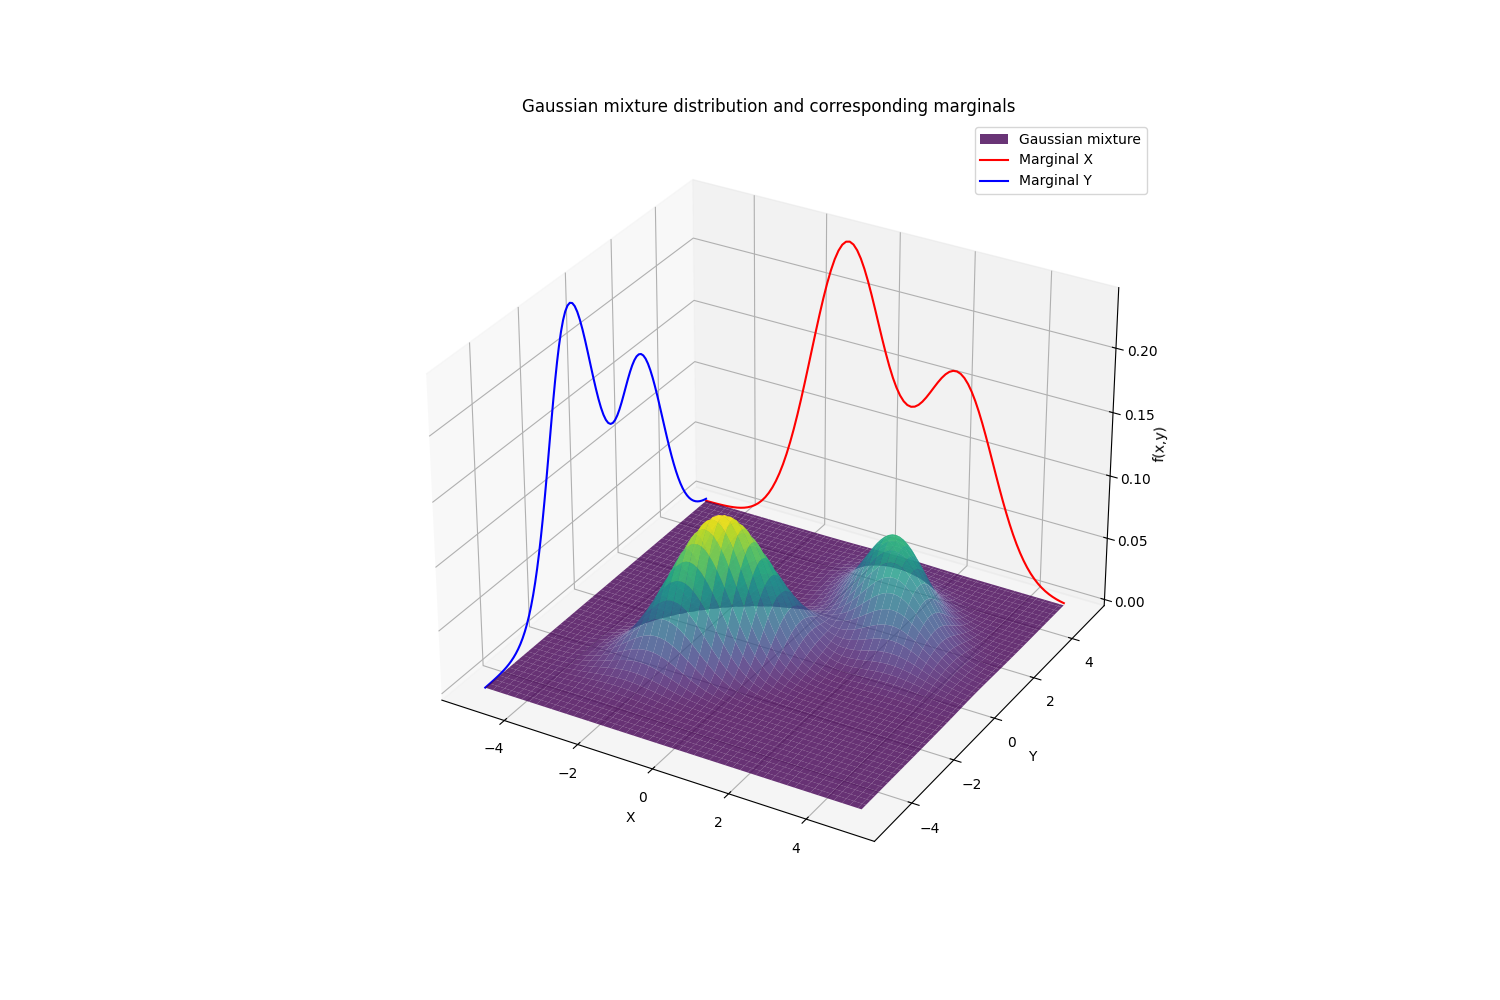
\includegraphics[width=1\textwidth]{text/chapter_01/imgs/gaussMix_with_marginals}
    \caption{Gaussian mixture distribution with means $\{[0,0], [2,2]\}$, weights $\{[0.6, 0.4]\}$ and corresponding marginals.}
    \label{fig:gaussMixWithMarginals}
\end{figure}

    \section{State-space model}
\label{sec:stateSpaceModel}
State-space models serve as a fundamental framework for describing the evolution of dynamic systems over time. In the context of multi-target tracking, state-space models provide a formalism for representing motion dynamics of targets and the measurement process, enabling an efficient and accurate inference of target states from sensor data.

At the core of a state-space model lies a set of latent variables, known as the state vector, which encapsulates the
unobservable quantities of interest, such as the position, velocity, and acceleration of targets in MTT. The dynamics governing the evolution of the state vector are typically described by a transition model, which specifies how the state evolves over time according to a probabilistic process. This transition model can take various forms depending on the nature of the system dynamics, ranging from simple linear or non-linear models to more complex stochastic processes.

In addition to the transition model, state-space models incorporate an observation model that describes the relationship between the observed measurements and the underlying state variables. This observation model accounts for the uncertainties and noise inherent in the measurement process, allowing for the probabilistic mapping of observed data to the latent state space.

State-space model can be represented as a pair of stochastic equations.
\begin{enumerate}
    \item \textbf{State transition equation:}
        \begin{align}
                  \mathbf{x_k} &= f(\mathbf{x_{k-1}}, \mathbf{u_k}, \mathbf{w_k}), \label{eq:state_space_model_state}
        \end{align}
        where $\mathbf{x_k}$ represents the state vector at time $k, f$ denotes the transition function describing the
        evolution of the state, $\mathbf{u_k}$ represents optional control inputs, and $\mathbf{w_k}$ denotes process
    noise.
    \item \textbf{Observation equation:}
        \begin{align}
            \mathbf{z_k} &= h(\mathbf{x_{k}}, \mathbf{v_k}), \label{eq:state_space_model_observation}
        \end{align}
        where $\mathbf{z_k}$ represents the observed measurements at time $k, h$ denotes the observation function
    mapping the
    state to measurements, and $v_k$ represents the measurement noise.
\end{enumerate}

In MTT, state-space models provide a natural framework for representing the motion dynamics of multiple targets and the sensor measurements associated with each target. Each target is typically associated with its own state vector, enabling simultaneous tracking of multiple objects within the same probabilistic framework.

State-space models enable MTT algorithms to perform a range of tasks, including target prediction, data association, and state estimation by propagating the state forward in time using the transition model and updating the state based on observed measurements using the observation model. By incorporating uncertainty explicitly into the tracking process, state-space models facilitate robust inference of target states in complex and dynamic tracking scenarios.

While state-space models offer a powerful framework for multi-target tracking, they also present several challenges.
\begin{itemize}
    \item \textbf{Model complexity:} Designing an appropriate state-space model requires careful consideration of the
    underlying dynamics and measurement process, which can be challenging in complex tracking scenarios with non-linearities and uncertainties.
    \item \textbf{Parameter estimation:} Estimating the parameters of a state-space model from data, such as the transition and observation matrices, can be computationally demanding and prone to issues such as overfitting or underfitting.
    \item \textbf{Computational Complexity:} Performing inference in state-space models often involves recursive algorithms such as the Kalman filter or the particle filter, which can be computationally intensive, especially in high-dimensional or real-time tracking applications.
\end{itemize}

Despite these challenges, state-space models remain a foundation of multi-target tracking, offering a principled and flexible framework for representing and reasoning about dynamic systems in the presence of uncertainty.
There are many state space models used in MTT. Before we define the two of the most common ones in the forthcoming sections, it
should be noted, that the definitions in \eqref{eq:state_space_model_state} and \eqref{eq:state_space_model_observation} are too general, because $f_k$ and $h_k$ could be any functions.

To get a closed-form solution in the Bayesian inference framework, we need
to choose conjugate distributions for the likelihood and the prior. The Kalman filter (see Section \ref{sec:Kalman} for
more) works for the Gaussian-linear case, where the functions
$f_t$ and $h_t$ represent linear and noisy variables and are distributed as Gaussians with zero mean. The Gaussian linear
state-space model has the formulation:
\begin{align}
    p(x_k|x_{k-1}) &= Fx_{k-1} + Bu_k + w_k
     &w_k \sim \mathcal{N}(0,Q),\\
    p(z_k|x_k) &= Hx_k + v_k
     &v_k \sim \mathcal{N}(0,R), \\
    p(x_0) &\sim \mathcal{N}(\hat{x}_0, P_0),
\end{align}
where
\begin{itemize}
    \item F is the transition matrix of appropriate dimension,
    \item B is the input matrix of appropriate dimension,
    \item H is the measurement matrix of appropriate dimension,
    \item Q is the symmetric positive semi-definite covariance matrix of
    motion noise $
    w_k$,
    \item R is the symmetric positive semi-definite covariance matrix of
    measurement
    noise $v_k$,
    \item $\hat{x}_0$ and $P_0$ are the mean and the covariance matrix of the prior state.
\end{itemize}
The control variable $u_k$, in general, represents some input signal from the environment, and
$B$ specifies how the input signal affects the dynamic system. This variable is usually not considered in MTT scenarios.
In multi-target tracking, Gaussian linear models are most often worked with, thus following formulation is used instead.
\begin{align}
    p(x_k|x_{k-1}) &= \mathcal{N}(x_k; Fx_{k-1}, Q),  \\
    p(z_k|x_k) &= \mathcal{N}(z_k;Hx_k,R), \\
    p(x_0) &\sim \mathcal{N}(x_0;\hat{x}_o, P_0).
\end{align}


    \subsection{Constant velocity model}
The constant velocity model (CVM) is a fundamental component of multi-target tracking systems, providing a simplified yet effective representation of target motion dynamics over time. This model assumes that the target's velocity remains constant between consecutive time steps, making it particularly suitable for tracking objects with relatively smooth and predictable motion patterns. In this section, we explore the conceptual basis, mathematical formulation, and practical implications of the constant velocity model in the context of MTT.

At its core, the constant velocity model embodies the notion of inertia, where a target maintains a constant velocity unless acted upon by external forces. This conceptual simplicity allows for a straightforward representation of target motion, making the constant velocity model a popular choice for MTT applications where targets exhibit relatively uniform and predictable movement behaviors.

Mathematically, the constant velocity model describes the evolution of a target's state vector over time in terms of
its position and velocity. At each time step $k$, the state vector $\mathbf{x}_k$ comprises the position $[x_{1,k},x_{
    2,k}]$ and velocity $s$ of the target
\begin{align}
    \mathbf{x}_k &= [x_{1,k}, x_{2,k}, s_{1,k}, s_{2,k}]^T.
\end{align}

The dynamics of the constant velocity model can be represented using a state transition matrix $F$  and a process
noise vector $w_k$, where the state transition matrix captures the relationship between the target's state at
consecutive time steps
\begin{align}
    \mathbf{x}_{k+1} &= \mathbf{F x}_k + \mathbf{w}_k.
\end{align}
All together, vector $\mathbf{x}_k$, matrices $\mathbf{F}$ and $\mathbf{Q}$, might, for example, be represented as
\begin{align}
    \mathbf{x}_k &=
        \begin{bmatrix}
            x_{1,k} \\
            x_{2,k} \\
            s_{1,k} \\
            s_{2,k} \\
        \end{bmatrix},
    \quad \mathbf{F} =
        \begin{bmatrix}
            1 & 0 & \Delta & 0 \\
            0 & 1 & 0 & \Delta \\
            0 & 0 & 1 & 0 \\
            0 & 0 & 0 & 1 \\
        \end{bmatrix},
    \quad \mathbf{Q} = q^2
        \begin{bmatrix}
            \frac{\Delta^3}{3} & 0 & \frac{\Delta^2}{2} & 0 \\
            0 & \frac{\Delta^3}{3} & 0 & \frac{\Delta^2}{2} \\
            \frac{\Delta^2}{2} & 0 & \Delta & 0 \\
            0 & \frac{\Delta^2}{2} & 0 & \Delta \\
        \end{bmatrix},
    \label{eq:state_space_model}
\end{align}
where $\Delta$ stands for delta time, i.e., elapsed time between the last estimation and the current one, $q$ is the
motion noise parameter, which represents the uncertainty in the state transition. The measurement model transforms a
state vector from the state-space into the measurement space. Since the filters derived from the Kalman filter assume only
linear models, the measurement model for CVM assumes the same space as in the state vectors. As a result, the
observation matrix $\mathbf{H}$ and the noise matrix $\mathbf{R}$ can be, with respect to \eqref{eq:state_space_model}, formulated
\begin{align}
    \mathbf{H} &=
    \begin{bmatrix}
        1 & 0 & 0 & 0 \\
        0 & 1 & 0 & 0 \\
    \end{bmatrix},
    \quad \mathbf{R} = r^2
    \begin{bmatrix}
        1 & 0  \\
        0 & 1  \\
    \end{bmatrix},
\end{align}
where $r$ determines the variance of the measurement noise.

To obtain optimal results given by filters, it is essential to set parameters $r$ and $q$ appropriately. There are
three main possible procedures. The first one requires the knowledge of motion noise given by tracked object and the
knowledge of sensor's error when detecting targets, i.e. the noisy measurement. This method is often used in
simulations and experiments. The second one is a simple trial
and error method with reasonable choices. The last one is using automated methods, like in \cite{BulutEastimation2011}.

By assuming the constant velocity, MTT
algorithms
can predict the future positions of targets based on their current state and velocity, facilitating trajectory estimation and target prediction.

One common application of the constant velocity model in MTT is in the design of prediction algorithms, where future positions of targets are estimated based on their current state and velocity information. These predictions are essential for anticipating target movements and facilitating data association, enabling the MTT algorithms to maintain track continuity and adapt to changes in the target behavior over time.

Moreover, the constant velocity model can be seamlessly integrated into recursive Bayesian filters, such as the Kalman filter, for state estimation in MTT. By incorporating the constant velocity model into the state-space representation of the tracking problem, Kalman filter-based algorithms can effectively fuse measurement information with dynamic predictions to estimate the most likely trajectories of targets over time.
    \subsection{Constant acceleration model}
The Constant Acceleration Model (CAM) stands as a sophisticated extension of the state-space model in multi-target
tracking, offering a more comprehensive representation of target motion dynamics. Unlike simpler models such as the Constant Velocity Model, which assumes a constant velocity for targets over time, the CAM acknowledges the potential for changes in target acceleration, allowing for more accurate and flexible trajectory estimation. This section delves into the conceptual basis, mathematical formulation, and practical implications of the Constant Acceleration Model in the context of MTT.

In MTT scenarios, targets often exhibit varying degrees of acceleration due to factors such as changes in speed,
direction, or environmental influences. Ignoring these accelerative effects can lead to biased trajectory estimates and diminished tracking accuracy. The CAM addresses this limitation by incorporating an additional acceleration component into the state-space model, enabling more faithful representation of target motion dynamics. By accounting for changes in acceleration, the CAM provides MTT algorithms with a greater flexibility and adaptability in tracking targets with non-uniform motion profiles.

Mathematically, the Constant Acceleration Model extends the state transition function of the state-space model to
accommodate changes in acceleration over time. At each time step $k$, the evolution of the target's state vector $x_k$ is governed by a set of dynamic equations that describe the position, velocity, and acceleration of the target
\begin{align}
    \mathbf{x}_k &= [x_{1,k}, x_{2,k}, s_{1,k}, s_{2,k}, a_{1,k}, a_{2,k}]^T,
\end{align}
where, as in CVM, $x_{1,k}$, $x_{2,k}$ is the position of an target in two-dimensional space, $s_{1,k}, s_{2,k}$ is
the velocity and $a_{1,k}, a_{2,k}$ are the accelerations in both directions. Matrices $F$ and $Q$ can then be expressed
\begin{align}
    \mathbf{x}_k &=
    \begin{bmatrix}
        x_{1,k} \\
        x_{2,k} \\
        s_{1,k} \\
        s_{2,k} \\
        a_{1,k} \\
        a_{2,k} \\
    \end{bmatrix},
    \quad \mathbf{F} =
    \begin{bmatrix}
        1 & 0 & \Delta & 0 & \frac{1}{2}\Delta^2 & 0\\
        0 & 1 & 0 & \Delta & 0 & \frac{1}{2}\Delta^2\\
        0 & 0 & 1 & 0 & 0 & 0\\
        0 & 0 & 0 & 1 & 0 & 0\\
        0 & 0 & 0 & 0 & 1 & 0\\
        0 & 0 & 0 & 0 & 0 & 1\\
    \end{bmatrix},
    \quad \mathbf{Q} = q^2
    \begin{bmatrix}
        \frac{\Delta^4}{4} & 0 & \frac{\Delta^3}{3} & 0 & \frac{\Delta^2}{2} & 0\\
        0 & \frac{\Delta^4}{4} & 0 & \frac{\Delta^3}{3} & 0 & \frac{\Delta^2}{2}\\
        \frac{\Delta^3}{3} & 0 & \frac{\Delta^2}{2} & 0 & \Delta & 0\\
        0 & \frac{\Delta^3}{3} & 0 & \frac{\Delta^2}{2} & 0 & \Delta \\
        \frac{\Delta^3}{3} & 0 & \frac{\Delta^2}{2} & 0 & \Delta & 0\\
        0 & \frac{\Delta^3}{3} & 0 & \frac{\Delta^2}{2} & 0 & \Delta \\
    \end{bmatrix}.
\end{align}
The measurement model remains unchanged from the standard state-space model, relating the observed measurements $\mathbf{z}_k$ to the target's true state $\mathbf{x}_k$ through a measurement function $h(\cdot)$ corrupted by measurement noise $v_t$
\begin{align}
    \mathbf{H} &=
    \begin{bmatrix}
        1 & 0 & 0 & 0 & 0 & 0 \\
        0 & 1 & 0 & 0 & 0 & 0 \\
    \end{bmatrix},
    \quad \mathbf{R} = r^2
    \begin{bmatrix}
        1 & 0  \\
        0 & 1  \\
    \end{bmatrix},
\end{align}
The Constant Acceleration Model offers several practical advantages in MTT applications:
\begin{itemize}
    \item \textbf{Improved trajectory estimation:} By accounting for changes in the acceleration, the CAM enables a more accurate
    and realistic trajectory estimation, particularly for targets exhibiting non-uniform motion patterns or sudden changes in velocity.
    \item \textbf{Enhanced predictive capability:} The inclusion of acceleration dynamics allows MTT algorithms to make more
    informed predictions about future target states, improving the tracking performance and reducing prediction errors.
    \item \textbf{Robustness to dynamic environments:} In dynamic environments with varying levels of congestion, obstacles,
    or traffic patterns, the CAM provides MTT algorithms with greater robustness and adaptability, enabling an effective tracking even in challenging scenarios.
    \item \textbf{Applications in autonomous systems:} In autonomous systems such as self-driving cars, drones, or robotics,
    the CAM plays a crucial role in motion planning, obstacle avoidance, and trajectory prediction, enhancing the safety and efficiency of an autonomous navigation.
\end{itemize}
In summary, the Constant Acceleration Model represents a significant advancement in multi-target tracking, offering a
more nuanced and comprehensive approach to modeling target motion dynamics. By incorporating acceleration effects
into the tracking process, the CAM enables MTT algorithms to achieve higher accuracy, robustness, and predictive capability, making it an indispensable tool for a wide range of applications.

    \section{Hidden Markov Model}
In the domain of multi-target tracking, the Hidden Markov Model (HMM) serves as a framework for
capturing the temporal dynamics of target behavior in complex environments. Building upon the principles of Markov
processes, the HMM extends the state-space model by introducing hidden states that govern the evolution of observable
measurements over time. Markov process of the first order is a model, in which current state depends only on the
previous state
\begin{align}
    p(x_k|x_1,\dots,x_{k-2},x_{k-1}, z_1, \dots, z_{k-2}, z_{k-1}) = p(x_k|x_{k-1}) &\quad \text{(transition
    probability)}, \\
    p(z_k|x_1,\dots,x_{k-2},x_{k-1}, x_k, z_1, \dots, z_{k-2}, z_{k-1}) = p(z_k|x_{k}) &\quad \text{(observation
    likelihood)}, \\
    p(x_0)& \quad \text{(initial state)}.
\end{align}
In models of higher order, the transition probability is
\begin{align}
    p(x_k|x_{k-1},\dots,x_{k-n}),
\end{align}
where $n$ is the number of the order. Details of this model are not described in this work and can be seen in \cite{
    HadarHMMHigherOrder}.

In cases where the process is not directly observable, but can be perceived through another observable variable $z_k$,
we often talk about Hidden Markov process.
\begin{figure}[h]
    \centering
    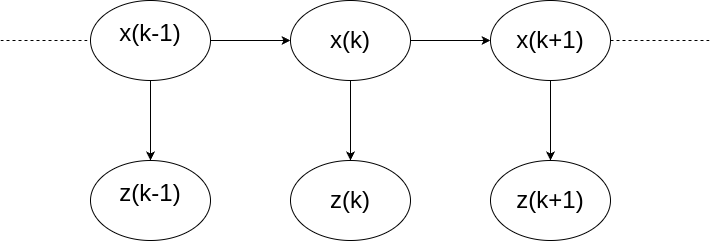
\includegraphics[width=0.8\linewidth]{./text/chapter_01/imgs/HMM}
    \caption{Demonstration of the course of the hidden Markov process.}
    \label{fig:hmm}
\end{figure}

At its base, the Hidden Markov Process represents a stochastic process characterized by a set of hidden states that transition probabilistically over time. While these hidden states are unobservable, they influence the generation of observable measurements, which are assumed to be conditionally independent given the hidden states. In the context of MTT, the hidden states may represent latent attributes of targets, such as their locations, velocities, or motion patterns, while the observable measurements correspond to sensor readings or detections obtained from surveillance systems.

\section{Bayes' filter}
The Bayes filter is a recursive framework that estimates an internal state of the system over time using measurements. The Bayes' filter leverages both motion and measurement models, operating under the assumption that these models
accurately describe the system's behavior. Operating within a recursive framework, the Bayes' filter continually
estimates the internal state of the system over time using available measurements. Each iteration of the filter
entails two fundamental steps: prediction and update. During the prediction step, the filter anticipates the internal
state $x_k$ based on the preceding state $x_{k-1}$ and the motion model $p(x_k|x_{k-1})$. This prediction step is
commonly referred to as the Chapman-Kolmogorov equation \cite{DedeciusSeq2017}.
\begin{theorem}[The Chapman-Kologorov equation prediction step]
    Given the set of measurements $z_{0:k-1} = {z_0,\dots, z_{k-1}}$, set of control variables $u_{0:k-1} = {u_0,\dots, u_{k-1}}$ and current state $x_{k-1}$ and the motion model $p(x_k|x_{k-1})$, the prediction step is as follows:
    \begin{align}
        p(x_k|z_{0:t-1}, u_{0:k}) &= \int p(x_k|x_{k-1}, u_k) p(x_{k-1}|z_{0:k-1}, u_{0:k-1}) dx_{k-1},
        \label{eq:chapman_kolmogorov_predict}
    \end{align}
    where the integral is taken over the entire state space of $x_{k-1}$, and $p(x_{k-1}|z_{0:k-1}, u_{0:k-1})$ is
    the posterior density of the state at time $k-1$.
\end{theorem}
During the update step, the Bayes' filter corrects (updates) the prediction step with measurements $z_k$ using the
measurement model $p(z_k|x_k)$. This step employs common Bayes' rule.
\begin{theorem}[The update step of Bayes' filter]
    Given the output of Bayes' filter's prediction step, the measurements $z_k$ observed at time $k$ and the
    measurement model $p(z_k|x_k)$, the update step of the Bayes' filter is formulated as follows:
    \begin{align}
        \label{eq:bayes_update}
        p(x_k|z_{0:t}, u_{0:t}) &= \frac{p(z_k|x_k) p(x_k|z_{0:k-1},u_{0:k})}{p(z_k|z_{0:k-1})} \propto p(z_k|x_k) p
        (x_k|z_{0:k-1},u_{0:k})
    \end{align}
\end{theorem}
These two steps work in an iterative method, where, in each iteration, the first prediction step is used to predict
the state $x_k$ and then the update step is used to correct our guess with the provided measurement.
\section{Kalman filter}
    \label{sec:Kalman}
The Kalman filter, named after its developer Rudolf E. Kalman, has a rich history dating back to the early 1960s when Kalman first introduced the algorithm in a series of landmark papers. Initially developed for aerospace applications, the Kalman filter gained prominence for its ability to provide an optimal state estimation in the presence of noisy measurements and uncertain dynamics.

Over the years, the Kalman filter has found widespread usage across diverse fields and industries, including aerospace, robotics, finance, and telecommunications. Its applications range from tracking spacecraft trajectories and guiding missiles to monitoring financial markets and controlling autonomous vehicles. The filter's versatility and efficiency have made it a cornerstone of modern estimation and control systems.

The Kalman filter operates on the principles of recursive Bayesian estimation, utilizing a system dynamics model and noisy measurements to predict and update the state of a dynamic system over time. Its mathematical elegance and simplicity make it well-suited for real-time applications, enabling an accurate and efficient state estimation even in complex and uncertain environments.

Despite its success, the Kalman filter continues to evolve, with extensions and variations such as the
extended Kalman filter (EKF), unscented Kalman filter (UKF), and particle filter (PF) addressing more challenging scenarios involving non-linear dynamics and non-Gaussian noise.

In summary, the Kalman filter stands as a seminal contribution to the field of estimation and control, with a rich history of development and widespread usage across diverse domains. Its continued relevance and versatility underscore its status as a foundational tool for state estimation and tracking in modern technological applications.

\subsection{Kalman filter inference}
In Section \ref{sec:stateSpaceModel} we talked about state-space model, which is used by the Kalman filter. Thus we work
with equations
\begin{align}
    x_k &= Fx_{k-1} + w_t \\
    z_t &= Hx_k + v_k,
\end{align}
where both noise variables are independent and with zero mean
\begin{align}
    w_k &\sim \mathcal{N}(0,Q), \\
    v_k &\sim \mathcal{N}(0,R).
\end{align}
Then the state and measurement distributions follows
\begin{align}
    x_k &\sim \mathcal{N}(Fx_{k-1},Q) \qquad && \text{with density}\quad p(x_k|x_{k-1}), \\
    z_k &\sim  \mathcal{N}(Hx_k,R) \qquad && \text{with density}\quad p(z_k|x_k).
\end{align}
Since the Kalman filter is Bayesian, we need a prior distribution for $x_k$. Model $z_k$ is Gaussian conjugate prior and
is then also a Gaussian with mean $x_{k-1}^+$ and covariance matrix $P_{k-1}^+$,
\begin{align}
    p(x_k|z_{0:k-1}) &= \mathcal{N}(x_{k-1}^+,P_{k-1}^+).
\end{align}

The prediction step is derived from Formula (\ref{eq:chapman_kolmogorov_predict}). Note, that by multiplying two
Gaussian distributions we again get the Gaussian distribution $\mathcal{N}(x_k^-,P_k^-)$ with hyperparameters
\begin{align}
    x_k^- &= Fx_{k-1}^+, \\
    P_k^- &= FP_{k-1}^{+}F^T + Q.
\end{align}
By multiplicating two Gaussian distributions followed by marginalization, we enumerate the state equation. The
estimation
of state $x_k^-$ is just applying model variables into appropriate equations. The estimated covariance $P_k^-$
expresses the degree of uncertainty of the estimation. By applying this step, the uncertainty grows.

The update step corrects the prediction step by applying new observed measurements $z_k$. For that, formula (\ref{eq:bayes_update}) is used. The model is transformed into an exponential form
\begin{align}
    p(z_k|x_k) &\propto \exp \left\{-\frac{1}{2}(z_k - Hx_k)^T R^{-1} (z_k - Hx_k)\right \} \nonumber \\
    &= \exp
    \left\{
        Tr\left(
        \underbrace{
            -\frac{1}{2}
            \begin{bmatrix}
                -1 \\
                x_k
            \end{bmatrix}
            \begin{bmatrix}
                -1 \\
                x_k
            \end{bmatrix}^T
        }_{\eta}
        \underbrace{
            \begin{bmatrix}
                z_k^T \\
                H^T
            \end{bmatrix}
            R^{-1}
            \begin{bmatrix}
                z_k^T \\
                H^T
            \end{bmatrix}^T
        }_{T(z_k)}
        \right)
    \right\}.
\end{align}
The conjugated shape has the form
\begin{align}
    p(x_k|z_{0:k-1}) &\propto \exp
    \left\{-\frac{1}{2}(x_k - x_k^-)^T (P_k^-)^{-1} (x_k - x_k^-)\right \} \nonumber \\
    &= \exp
    \left\{
    Tr\left(
    \underbrace{
        -\frac{1}{2}
        \begin{bmatrix}
            -1 \\
            x_k
        \end{bmatrix}
        \begin{bmatrix}
            -1 \\
            x_k
        \end{bmatrix}^T
    }_{\eta}
    \underbrace{
        \begin{bmatrix}
            (x_k^-)^T \\
            I
        \end{bmatrix}
        (P_k^-)^{-1}
        \begin{bmatrix}
            (x_k^-)^T \\
            I
        \end{bmatrix}^T
    }_{\xi_k}
    \right)
    \right\},
\end{align}
where $I$ is an identity matrix of appropriate shape.

The bayesian update is a sum of the hyperparameter and sufficient statistic,
\begin{align}
    \xi_{k}
    &= \xi_{k-1} +  T(z_{k})  \nonumber \\
    &=
    \begin{bmatrix}
    (x_{k}^{-})^{T} (P_{k}^{-})^{-1} x_{k}^{-} + z_{k}^{T} R^{-1} z_{k},
    & (x_{k}^{-})^{T} (P_{k}^{-})^{-1} + z_{k}^{T} R^{-1} H \\
    (P_{k}^{-})^{-1} (x_{k}^{-})^{T} + H^{T} R^{-1} z_{k},
    & (P_{k}^{-})^{-1} + H^{T} R^{-1} H.
    \end{bmatrix}
\end{align}
The posterior parameters are then derived
\begin{align}
    P_{k}^{+} &= (\xi_{k;[2,2]})^{-1} \notag\\
    &= \left[ (P_{k}^{-})^{-1} + H^{T} R^{-1} H \right]^{-1} \notag\\
    &= (I - K_{k} H) P_{k}^{-} \\
    x_{k}^{+} &= (\xi_{k;[2,2]})^{-1} \xi_{k;[2,1]} \notag\\
    &= P_{k}^{+} \left[ (P_{k}^{-})^{-1} (x_{k}^{-})^{T} + H^{T} R^{-1} z_{k}\right] \notag \\
    &= x_{k}^{-} + P_{k}^{+} H^{T} R^{-1}(z_{k} - Hx_{k}^{-}),
\end{align}
where
\begin{align}
    K_{k} &= P_{k}^{-} H^{T}(R + H P_{k}^{-}H^{T})^{-1} \label{eq:kalman_gain}
\end{align}
is the Kalman gain. This form is the optimal Kalman gain, as it minimizes the root mean squared error. In general, the
greater the gain, the greater the emphasis of the new measurements. The filter then becomes more sensitive.

There are several possible formulas that express the optimal Kalman filter. One of the most popular formulations is
as follows:
\begin{align}
    \hat{z}_{k}^{-} &= H \hat{x}_{k}^{-}, \qquad &&\text{(measurement prediction)} \\
    \nu_t &= z_t - \hat{z}_{k}^{-}, \qquad &&\text{(innovation or prediction error $z_t$)} \\
    S_t &= H P_{k}^{-} H^T + R, \qquad &&\text{(covariance of innovation $\nu_t$)} \\
    K_t &= P_{k}^{-} H^T S_t^{-1}, \qquad &&\text{(Kalman gain)} \\
    {x}_{k}^{+} &= \hat{x}_{k}^{-} + K_t \nu_t, \qquad &&\text{(posterior state estimation $x_t$)} \\
    P_{k}^{+} &= (I - K_t H) P_{k}^{-}. \qquad &&\text{(posterior covariance)}
\end{align}

The pseudo-algorithm of Kalman filter is shown in Algorithm \ref{alg:kalman_filter}.
\begin{algorithm}
    \caption{Kalman Filter Algorithm}
    \begin{algorithmic}[1]
        \State \textbf{Inputs:} Initial state estimate $\hat{x}_0$, initial covariance matrix $P_0$, system
        dynamics matrix $F$, process noise covariance matrix $Q$, measurement matrix $H$, measurement noise
        covariance matrix $R$, and measurements $Z$.
        \State \textbf{Outputs:} Updated state estimate $\hat{x}_k$ and updated covariance matrix $P_k$.
        \State
        \Procedure{Initialization}{$x_0,P$}
            \State $\hat{x}_0 = x_0$  \Comment{Initialize state estimate}
            \State $P_0 = P$ \Comment{Initialize error covariance matrix}
        \EndProcedure

        \State
        \Procedure{Prediction step}{}
            \State $\hat{x}_{k|k-1} = F \hat{x}_{k-1} $ \Comment{Predict state estimate}
            \State $P_{k|k-1} = F P_{k-1} F^T + Q$ \Comment{Predict covariance:}
        \EndProcedure

        \State
        \Procedure{Update step}{$z_k$}
            \State $K_k = P_{k|k-1} H^T (H P_{k|k-1} H^T + R)^{-1}$ \Comment{Kalman gain}
            \State $\hat{x}_k = \hat{x}_{k|k-1} + K_k(z_k - H \hat{x}_{k|k-1})$ \Comment{Update state estimate}
            \State $P_k = (I - K_k H) P_{k|k-1}$ \Comment{Update covariance}
        \EndProcedure
        \State
        \Procedure{Kalman filter recursion}{}
            \State Initialization
            \ForAll{z_k $ \in$ Z}
                \State Perform Prediction Step
                \State Perform Update Step with $z_k$
            \EndFor
        \EndProcedure

    \end{algorithmic}
    \label{alg:kalman_filter}
\end{algorithm}
\chapter{Target tracking}
Target tracking plays a pivotal role in radar systems, where the primary objective is to estimate the trajectory and characteristics of moving objects within a surveillance area. Derived from the foundational principles of the Kalman filter, target tracking algorithms are tailored to the specific requirements and challenges inherent in radar applications.

Radar-based target tracking encounters various complexities, including survivability and the presence of crossing targets. Survivability concerns the algorithm's ability to maintain accurate estimates despite target maneuvers, occlusions, or potential target loss. Furthermore, the phenomenon of crossing targets introduces significant ambiguities and challenges in trajectory estimation and association.

In the realm of single-target tracking, algorithms such as the Probabilistic Data Association (PDA) filter and its derivatives, such as the Joint Probabilistic Data Association (JPDA) filter or the Integrated Probabilistic Data Association (IPDA) filter, are commonly employed. These algorithms provide robust solutions for associating measurements with existing tracks and updating target state estimates in dynamic scenarios.

Beyond single-target tracking, radar systems often necessitate multi-target tracking approaches. These approaches, particularly those based on Random Finite Sets (RFS), offer advanced capabilities for tracking multiple targets simultaneously. RFS-based filters, including the Probability Hypothesis Density (PHD) filter and the Multi-Bernoulli filter, excel in scenarios where the number of targets is uncertain or dynamic.

In this chapter, we delve into the intricacies of radar-based target tracking algorithms, exploring their theoretical foundations, practical implementations, and performance characteristics. By understanding the diverse range of tracking algorithms available and their respective strengths, we can design and deploy effective tracking systems to meet the demands of modern surveillance and reconnaissance applications.

\section{Data association}
\label{sec:data_association}
Data association uncertainty arises in remote sensing systems, such as radar, sonar, or electro-optical devices, when
measurements are obtained from sources that may not necessarily be the target of interest \cite{BarShalomPDA}. This uncertainty
occurs particularly in situations where the target signal is weak, necessitating a lower detection threshold, which may result in the detection of background signals, sensor noise, or clutter. Additionally, data association uncertainty can occur when multiple targets are present in close proximity. Utilizing spurious measurements in a tracking filter can lead to divergence of the estimation error and, consequently, track loss.

Addressing this challenge involves two primary problems. The first is the selection of appropriate measurements to update the state of the target of interest in the tracking filter, which can be a Kalman filter or an extended Kalman filter (EKF). The second problem involves determining whether the filter needs modification to account for data association uncertainty. The objective is to obtain the minimum mean square error (MMSE) estimate of the target state and associated uncertainty.

The optimal estimator involves the recursive computation of the conditional probability density function (pdf) of the
state, with detailed conditions provided under which this pdf serves as a sufficient statistic in the presence of
data association uncertainty.
  \subsection{Validation region}
    \label{sec:validation_region}
In target-tracking scenarios, the process of signal detection provides measurements, from which the appropriate ones for inclusion in the target state estimator are chosen. In radar systems, for instance, the signal reflected from the target of interest is sought within a specific time interval, determined by the expected range of the target when it reflects the transmitted energy. A range gate is established, and detections falling within this gate can be associated with the target of interest. These measurements may include parameters such as range, azimuth, elevation, or direction cosines, and in certain cases, range rate for radar or active sonar; bearing, and potentially frequency, time difference of arrival, and frequency difference for passive sonar; as well as line-of-sight angles or direction cosines for optical sensors. By setting up a multidimensional gate, the signal from the target is detected efficiently, avoiding the need to search for it across the entire measurement space.

However, while a measurement within the gate is a candidate for association with the target, it is not guaranteed to have originated from the target itself. Thus, the establishment of a validation region becomes necessary. The validation region is designed to ensure that the target measurement falls within it with a high probability, known as the gate probability, based on the statistical characterization of the predicted measurement. In the event that more than one detection appears within the gate, association uncertainty arises. This uncertainty entails the need to determine which measurement is truly from the target and should therefore be utilized to update the track, which comprises the state estimate and covariance, or more generally, the sufficient statistic for the target in question. Measurements outside the validation region can be disregarded, as they are too distant from the predicted measurement and are unlikely to have originated from the target of interest. This scenario typically arises when the gate probability is close to unity, and the statistical model used to define the gate is accurate.
\section{Clutter}
When it comes to clutter, two scenarios may occur. The first one is a single target in a clutter. This problem of
tracking a single target in a clutter appears when several measurements appear in the validation region. The
validated measurements comprise the accurate measurement, if detected within this region, along with spurious
measurements originating from clutter or false alarms. In air traffic control systems, where cooperative targets are
involved, each measurement includes a target identifier known as the squawk number. If this identifier is entirely
reliable, data association uncertainty is eliminated. However, in cases where a potentially hostile target is non
-cooperative, data association uncertainty becomes a significant challenge.

Figure \ref{fig:singleTargetInClutter} illustrates a scenario involving multiple validated measurements. The validation region depicted in the
figure is two-dimensional and takes the form of an ellipse centered at the predicted measurement $\hat{z}$. The
elliptical shape of the validation region arises from the assumption that the error in the target's predicted
measurement, known as the innovation, follows a Gaussian distribution. The parameters defining the ellipse are
determined by the covariance matrix $S$ of the innovation.

All measurements within the validation region have the potential to originate from the target of interest, although
only one of them is the true measurement. As a result, the possible association events include: $z_1$ originating
from the target, with $z_2$ and $z_3$ being from clutter; $z_2$ originating from the target, with $z_1$ and $z_3$
being from clutter; $z_3$ originating from the target, with $z_2$ and $z_1$ being from clutter; or all measurements
being from clutter. These association events are mutually exclusive and exhaustive, enabling the application of the
total probability theorem to obtain the state estimate in the presence of data association uncertainty.

Under the assumption of a single target, the spurious measurements are considered random interference. A common model for such false measurements assumes that they are uniformly spatially distributed and independent across time, corresponding to residual clutter. Any constant clutter is assumed to have already been removed.

\begin{figure}[h]
  \centering
  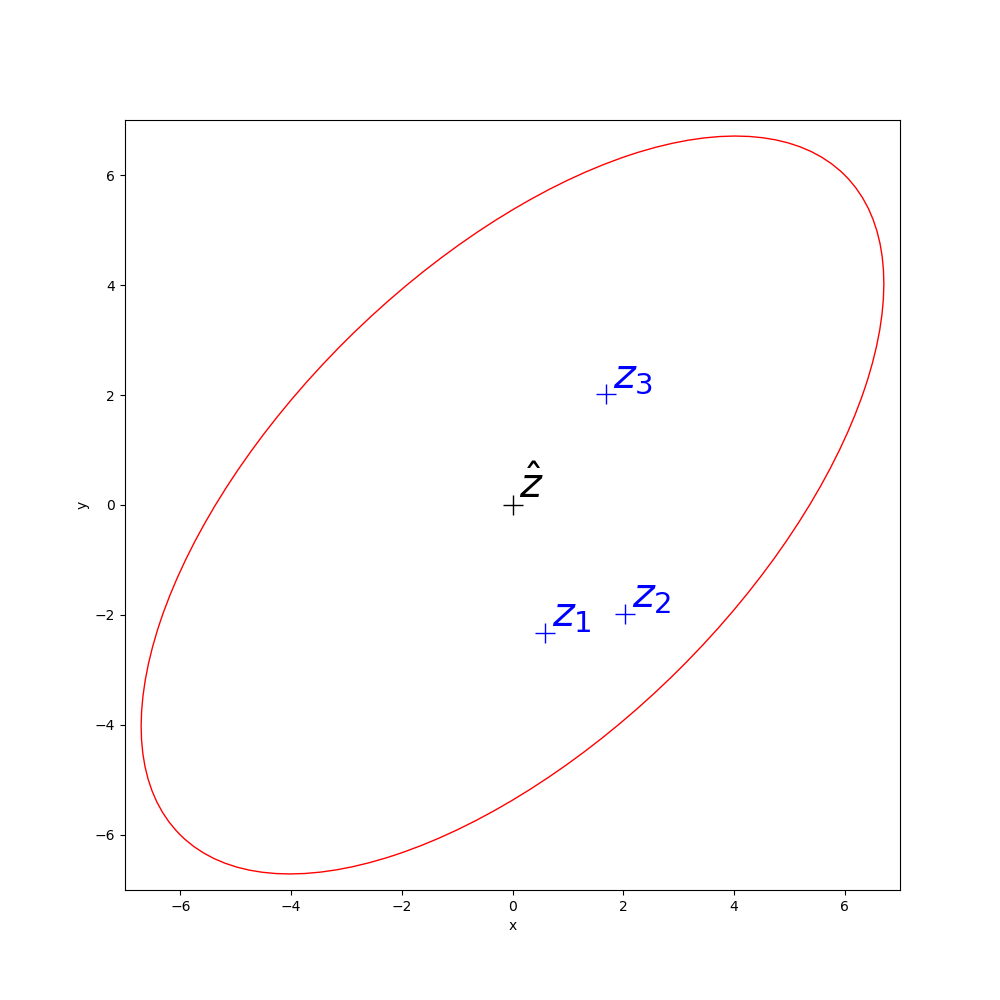
\includegraphics[width=10cm]{text/chapter_02/imgs/clutter_singleTarget}
  \caption{Several measurements $z_i$ appeared in the validation region of a single target. $\hat{z}$ is a predicted
  measurement and none or any of the measurement $z_1 - z_3$ may have originated from the target.}
  \label{fig:singleTargetInClutter}
\end{figure}

When several targets as well as a clutter or false alarms appear in the same neighbour, the data association becomes even more challenging. Figure \ref{fig:twoTargetsInClutter} shows this scenario, where predicted measurement for the targets are close to each other. These predicted points are labeled as $\hat{z_1}$ and $\hat{z_2}$. In This Figure many association combinations are possible; $z_1$ from target $\hat{z_1}$ or clutter; $z_2$ from target $\hat{z_1}$ or clutter; $z_4$ from target $\hat{z_2}$ or clutter; $z_3$ from target $\hat{z_1}$ or targe $\hat{z_2}$ or clutter. However, if $z_3$ originated from target $\hat{z_1}$, then it probable, that $z_4$ originated from target $\hat{z_2}$.

This scenario demonstrates the intricate relationships among associations when persistent interference from neighboring targets coexists with random interference or clutter. In such cases, joint association events become necessary to properly account for these dependencies.

A more complex scenario may arise due to the inherent finite resolution capability of signal processing systems. While each measurement is typically assumed to originate from either a target or clutter, an additional possibility must be considered: the merging of detections from multiple targets. Specifically, measurement $z_3$ could potentially result from such merging, representing an unresolved measurement. This introduces a fourth origin hypothesis for a measurement lying within the intersection of two validation regions.

The discussion highlights the challenges associated with associating measurements to tracks. The complete problem involves associating measurements at each time instant, updating the track's sufficient statistic, and propagating it to the subsequent time instant.

\begin{figure}[h]
    \centering
    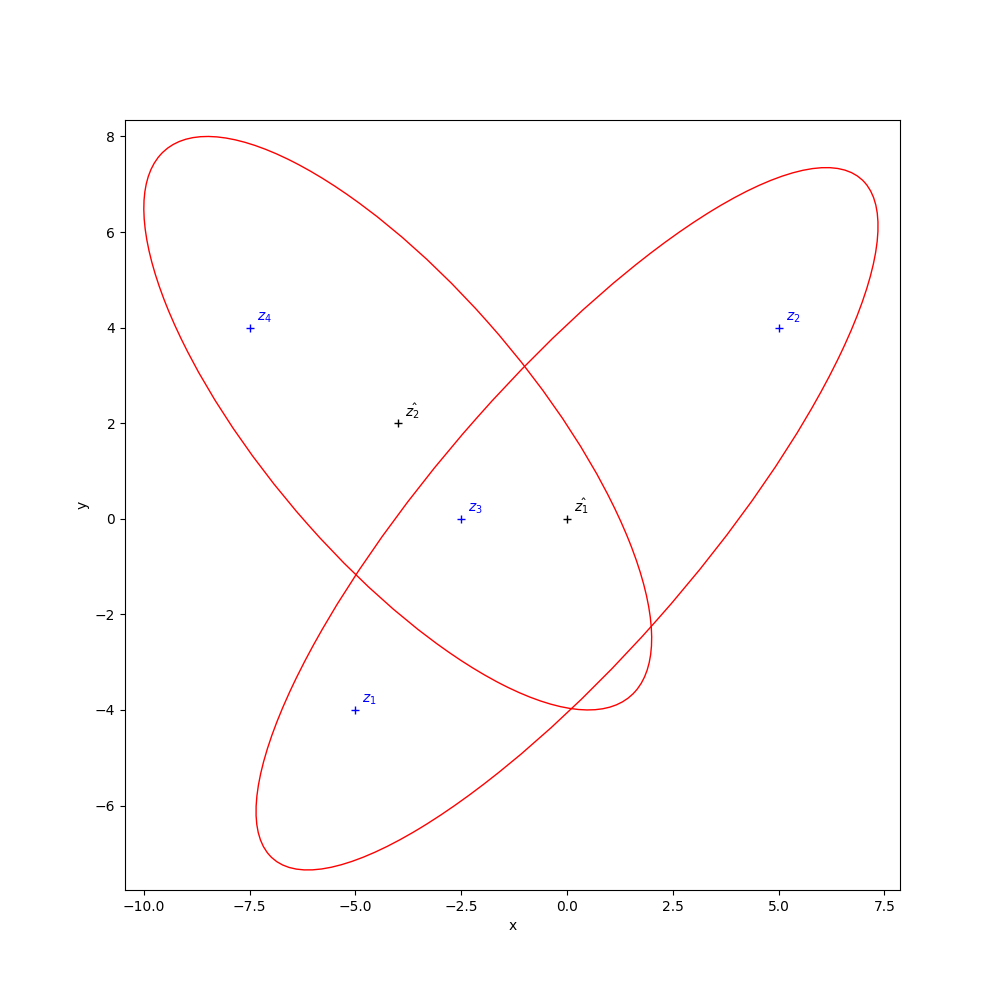
\includegraphics[width=10cm]{text/chapter_02/imgs/clutter_multiTarget}
    \caption{Several measurements $z_i$ appeared in the validation region of one of targets $\hat{z_1}$ or $\hat{z_2}$. $\hat{z_1}$ and $\hat{z_2}$ are predicted
    measurements and none or any of the measurement $z_1 - z_3$ may have originated from the target $\hat{z_1}$ and none or any of the measurement $z_3 - z_4$ may have originated from the target $\hat{z_2}$.}
    \label{fig:twoTargetsInClutter}
\end{figure}


\section{Single target tracking}
Single Target Tracking algorithms are specifically designed to track a single target amidst clutter and other sources of interference. Unlike conventional Kalman filters, which are not inherently equipped to handle clutter, Single Target Tracking algorithms incorporate mechanisms to enhance target survivability in cluttered environments.

One prominent algorithm in the data association category of target tracking is the Probabilistic Data Association (PDA) filter. The PDA filter addresses the challenge of associating measurements with the correct target while accounting for data association uncertainty. This uncertainty arises from the presence of clutter and the possibility of spurious measurements.


\subsection{PDA filter}
\label{sec:pda_filter}
The Probabilistic Data Association (PDA) algorithm computes the association probabilities for each validated measurement at the current time with respect to the target being tracked. This probabilistic or Bayesian information serves as a foundation for the Probabilistic Data Association Filter (PDAF) tracking algorithm, which effectively addresses the uncertainty regarding the origin of measurements. In scenarios where the state and measurement equations are linear, the resulting PDAF algorithm operates based on the Kalman Filter (KF). However, if the state or measurement equations are nonlinear, the PDAF algorithm is instead based on the Extended Kalman Filter (EKF). This adaptation allows the PDAF algorithm to accommodate nonlinearity in the system dynamics or measurement processes, ensuring robust performance in diverse tracking scenarios.

The PDAF algorithm comes with many assumptions:
\begin{enumerate}
    \item Only one target of interest is present, whose state $x \in R^{n_x}$ is assumed to evolve in time according to the equation
        \begin{align}
            x_k &= F_{k-1} x_{k-1} + \mu_{k-1},
        \end{align}
        with the true measurement $z_k \in R^{n_z}$ given by
        \begin{align}
            \label{eq:pda_A1_eq2}
            z_k &= H_k x_k + w_k,
        \end{align}
        where $\mu_{k-1}$ and $w_k$ are zero mean mutually independent, white Gaussian noise variables with covariances $Q_{k-1}$ and $R_k$, respectively.
    \item The track has been initialized.
    \item The past information through time $k-1$ about the target is summarized approximately by a suffifient statistic in the form of the Gaussian posterior
        \begin{align}
            p(x_{k-1}|z_{k-1}) &= \mathcal{N}(x_{k-1}; x_{k-1|k-1}, P_{k-1|k-1})). \label{eq:pda_A3}
        \end{align}
    \item At each time a measurement validation region is set up around the predicted measurement to select the candidate measurements for association to the target of interest.
    \item If the target was detected and the corresponding
    measurement fell into the validation region, then,
    according to (\ref{eq:pda_A1_eq2}), at most one of the validated measurements can be target originated.
    \item The remaining measurements are assumed to be due
    to false alarms or clutter and are modeled as inde-
    pendent and identically distributed with uniform spatial distribution, and the number of false alarms or clutter points obeys either a Poisson distri-
    bution, that is, a spatial Poisson process, with known
    spatial density $\lambda$, or a diffuse prior.
    \item The target detections occur independently over time
    with known probability $p_D$.
\end{enumerate}
All these assumptions make a filter a for state estimation, that is almost as simple as Kalman filter, but more effective in the presence of clutter.

As well as the Kalman Filter, the PDAF also consists of prediction and update step. Before the update step, two additional steps occur - measurement validation and data association. 
 \subsubsection{PDAF predict step}
The prediction step of PDA filter from time $k-1$ to $k$ is as in the standard KF,
\begin{align}
    x_{k|k-1} &= F_{k-1}x_{k-1|k-1},\\
    \eta_{k|k-1} &= H_k x_{k|k-1},\\
    P_{k|k-1} &= F_{k-1} P_{k-1|k-1} F_{k-1}^T + Q_{k-1},
\end{align}
where $P_{k-1|k-1}$ is from equation (\ref{eq:pda_A3}). The innovation covariance matrix $S_k$ is computed as
\begin{align}
    S_k &= H_{k} P_{k|k-1} H_{k}^T + R_{k}. \label{eq:pda_S}
\end{align}

\subsubsection{PDAF measurement validation step}
As discussed in Section \ref{sec:validation_region}, the measurements considered to be originated from given target should fall into validation region. This elliptical region is formulated as
\begin{align}
    \nu(k,\gamma) &= \bigcup_{z \in Z_k}[(z - \hat{z}_{k|k-1})^T S_k^{-1} (z - \hat{z}_{k|k-1})) \leq \gamma], \label {eq:validation_region}
\end{align}
where $Z_k$ are all measurements at time $k$, $\gamma$ is the gate threshold corresponding to the gate probability $p_G$, which is the probability, that the region contains the correct measurement if detected and $S_k$ given in (\ref{eq:pda_S}) is the covariance of the innovation.

\subsubsection{PDAF data association step}
The clutter in target tracking is assumed to be Poisson model with spatial density $\lambda$. In PDAF it yields to the association probability for $z_{i,k}$ being the correct measurement as

\vspace{-0.5cm}

\begin{align}
    \beta_{i,k} &=
    \begingroup
    \Large
    \begin{cases}
        \frac{\mathcal{L}_{i,k}}{1-p_D p_G + \sum_{j=1}^{m_k}\mathcal{L}_{j,k}}, & i=1, \dots, m_k, \\
        \frac{1-p_D p_G}{1-p_D P_G + \sum_{j=1}^{m_k}\mathcal{L}_{j,k}}, & i =0,
    \end{cases}
    \label{eq:pda_beta}
    \endgroup
\end{align}
where $i=0$ means none is correct, $p_D$ is the detection probability, $p_G$ is the gate probability analogous to (\ref{eq:validation_region}), and
\begin{align}
    \mathcal{L}_{i,k} &= \frac{\mathcal{N}(z_{i,k};\hat{z}_{k|k-1}, S_k) p_D}{\lambda} \label{eq:pda_likelihood}
\end{align}
is the likelihood ratio of the measurement $z_{i,k}$ from the validation region. The parameter $\lambda$ (the density of the spation Poisson clutter process) in the denominator of (\ref{eq:pda_likelihood}) models the clutter density of the uniform pdf of the location of false measurement. The Probabilistic Data Association (PDA) algorithm produces association probabilities that are influenced by the position of the respective innovation on the Gaussian exponential of the likelihood ratio (\ref{eq:pda_likelihood}), in comparison to other innovations.

\subsubsection{PDAF update step}
The update step equation of update step is
\begin{align}
    \hat{x}_{k|k} &= \hat{x}_{k|k-1} + K_k \nu_k, \label{eq:pda_update_state}
\end{align}
where the combined innovation is
\begin{align}
    \nu_k &= \sum_{i=1}^{m_k} \beta_{i,k} \nu_{i,k}
\end{align}
and the Kalman gain is the same as in (\ref{eq:kalman_gain})
\begin{align}
    K_k &= P_{k|k-1} H_k^T S_k^{-1}.
\end{align}
The covarince matrix associated with the update state (\ref{eq:pda_update_state}) is
\begin{align}
    P_{k|k} &= \beta_{0,k} P_{k|k-1} + (1-\beta_{0,k}) P_{k|k}^c + \tilde{P}_k,
\end{align}
where the covariance of the updated state with the corrected measurement is
\begin{align}
    P_{k|k}^c &= P_{k|k-1} - K_k S_k K_{k}^T, \label{eq:pda_update_cov}
\end{align}
and the spread of the innovation term is
\begin{align}
    \tilde{P}_k &= K_k (\sum_{i=1}^{m_k} \beta_{i.k} \nu_{i,k} \nu_{i,k}^T - \nu_{i,k} \nu_{i,k}^T) K_k^T. \label{eq:pda_covariance_increase}
\end{align}
With probability $\beta_{0,k}$ none of the measurement is correct. In such case, there is not update step of the
state estimation. The prediction covariance $P_{k|k-1}$ in (\ref{eq:pda_update_cov})) has weight $\beta_{0,k}$. There is probability $1-\beta_{0,k}$ that correct measurement appears and the update covariance $P_{k|k}^c$ has weight $1-\beta_{0,k}$. However, there is not certainty, which of the validated measurement $m_k$ is correct, the positive semidefinite matrix increases the covariance. This matrix is the result of the measurement origin uncertainty. Note, that in (\ref{eq:pda_covariance_increase}) the dependende of the estimation is nonlinear. The PDAF is nonlinear estimator, while the estimate update in (\ref{eq:pda_update_state}) appears linear, but the association probabilities $\beta_{i,k}$ depend on the innovation in (\ref{eq:pda_beta}).



\section{Multi target tracking}
In the field of multi-target tracking, there are many different algorithms and approaches. One of the classes is the particle filters approach (\cite{Particle_Khan2005, Particle_Gustafsson2002, Particle_Doucet2001,nonlinearParticleFilter}). These filters are able to handle nonlinear motion, but the computational demands are really high. The second class is bayesian filtering, which usually is more effective when it comes to computational power. Moreover there are two different approaches - data association filters and random finite sets (RFS) filters. The example of data association, which we talked about in section \ref{sec:data_association}, is the PDA filter (\ref{sec:pda_filter}) or the integrated probabilistic data association filter. The updated version of these filters, that can handle more targets, especially when two or more targets' validation region is in the same neighbourhood are the joint probabilistic data association (JPDA) filter and the joint integrated probabilistic data association (JIPDA) filter. The other family is filters based on random finite sets. Random finite sets statistics are explained in the following section.
%    \subsection{JPDA filter}
%    \subsection{IPDA filter}
    \subsection{RFS statistics}
Multitarget tracking presents challenges in estimating the states of multiple dynamic objects over time, complicated by varying target numbers, cluttered sensor measurements, and data association ambiguity. Traditional tracking frameworks rely on explicit associations between measurements and targets, leading to computational complexities, particularly in scenarios with high target densities and clutter rates.

Recent advancements introduce Random Finite Set (RFS) theory as an alternative approach to multitarget tracking. RFS theory represents sets with random cardinalities and values, offering a flexible framework for modeling uncertain multitarget scenarios. By treating both the multitarget state and sensor measurements as RFS, tracking algorithms can capture uncertainties effectively.

In scenario with more targets, i. e., multitarget scenario, let $M(k)$ be the number of targets at time $k$. At time $k-1$ the target states are $x_{k-1,1}, \dots, x_{k-1,M(k-1)} \in \mathcal{X}$. At the following time step $k$, some of these targets may disappear, some may evolve to their new states and also some new targets may be borned. As a result we have $M(k)$ targets with states $x_{k,1},\dots, x_{k,M(k)} \in \mathcal{X}$. The RFS model formulation ensures, that the order in which the states are listed has no significance. Also, at time $k$, $N(k)$ measurements $z_{k,1},\dots,z_{k,N(k)} \in \mathcal{Z}$ are received by the sensors, but the origins of these measurements are not known and the RFS model again ensures, that the order in which the measurements came has no significance. Some of these measurements are generated by the targets, some are only false measurements, i. e., clutter.

The goal of multiple-target tracking is to collectively estimate both the quantity of targets and their respective states using measurements of uncertain origin. Even under ideal circumstances where the sensor detects all targets without clutter, single-target filtering techniques are inadequate due to the absence of information regarding the origin of each observation.

Given the absence of inherent ordering within the sets of target states and measurements at a specific time, they can be naturally depicted as finite sets, denoted as
\begin{align}
    X_k &= \{x_{k,1},\dots, x_{k,M(k)}\} \in \mathcal{F}(\mathcal{X}) \\
    Z_k &= \{z_{k,1},\dots, z_{k,N(k)}\} \in \mathcal{F}(\mathcal{Z}),
\end{align}
where $\mathcal{F}(\mathcal{X})$ and $\mathcal{F}(\mathcal{Z})$ are collections of all finite subsets of $\mathcal{X}$ and $\mathcal{Z}$, respectively. In the random finite set approach, we consider the sets of targets and measurements, denoted as $X_k$ and $Z_k$ respectively, as the state and observation in multiple-target tracking. This perspective allows us to frame the multiple-target tracking problem as a filtering task with a state space $\mathcal{F}(x)$ and an observation space $\mathcal{F}(Z)$.

In a scenario with a single target, uncertainty is typically represented using random vectors to model the state $x_k$ and the measurement $z_k$. Similarly, in a multiple-target scenario, we represent uncertainty by using random finite sets to model the multiple-target state $X_k$ and the multiple-target measurement $Z_k$. An RFS $X$ is essentially a random variable that takes on finite sets of values, described by a discrete probability distribution and a set of joint probability densities. The distribution specifies the number of elements in $X$, while the densities describe the distribution of these elements.

We now delve into an RFS-based model for the evolution of the multiple-target state, taking into account target motion,
birth, and death. Given a multiple-target state $X_{k-1}$ at time $k-1$, each individual target $x_{k-1} \in X_{k-1}$ either remains present at time $k$ with probability $p_{S,k}(x_{k-1})$ or disappears with probability $1 - p_{S,k}(x_{k-1})$. If the target continues to exist, the probability density of transitioning from state $x_{k-1}$ to $x_k$ is denoted by $f_{k|k-1}(x_k|x_{k-1})$. Consequently, for each state $x_{k-1} \in X_{k-1}$ at time $k-1$, its behavior in the subsequent time step is modeled as the RFS
\begin{align}
    S_{k|k-1}(x_{k-1}),
\end{align}

that can represent two scenarios: either the survival of a target, indicated by the set $\{x_k\}$, or the absence of a
target, denoted by $\emptyset$, implying the target's demise.

The occurrence of a new target at time $k$ can originate from two possibilities: spontaneous births, which are independent of any existing target, or the spawning from a target present at time $k-1$.

Given a multiple-target state $X_{k-1}$ at time $k-1$, the state $X_k$ at time $k$ is formulated as the union of
surviving targets, newly spawned targets, and spontaneously born targets

\begin{align}
    X_k &= \left[\bigcup_{\zeta \in X_{k-1}}S_{k|k-1}(\zeta) \right] \cup \left[ \bigcup_{\zeta \in X_{k-1}} B_{k|k-1}(\zeta) \right] \cup \Gamma_k, \label{eq:rfs_state_union}
\end{align}
where
\begin{itemize}
    \item $\Gamma_k$ is RFS of spontaneous births at time $k$,
    \item $B_{k|k-1}(\zeta)$ is RFS of targets spawned at time $k$ from a target with previous state $\zeta$.
\end{itemize}
It is also assumed that RFSs in \ref{eq:rfs_state_union} are independent of each other, but the forms of $\Gamma_k$
and $B_{k|k-1}(\cdot)$ are problem dependent.

The measurement sets $Z_k$ are also random finite sets including detection uncertainty and clutter. A target $x_k \in X_k$ can be either detected with probability $p_{D,k}(x_k)$ or not detected with probability $1-p_{D,k}(x_k)$. Moreover, at time $k$, each state $x_k$ produces an RFS
\begin{align}
    \Theta_k(x_k)
\end{align}
that is ${z_k}$ in a case when the target is detected or $\emptyset$ otherwise. Furthermore, the sensor not only
receives measurements originated from targets, but also a set $K_k$, which are false measurements (clutter). Thus, at
time $k$, the multi-target measurement set $Z_k$ observed by the sensor is also formulated as a union of measurements
originated from targets and clutter
\begin{align}
    Z_k &= \left[ \bigcup_{x \in X_k} \Theta_k(x) \right] \cup \mathcal{K}_k. \label{eq:rfs_measurement_union}
\end{align}
The RFSs are assumed to be independent of each other and the actual form of $K_k$ is problem dependent.


Finite Set Statistics (FISST) is fundamental within the RFS framework, providing a systematic way to apply RFS theory
to multitarget tracking. FISST extends Bayesian filtering techniques to multitarget scenarios, enabling rigorous
estimation of multitarget states in the presence of clutter and data association uncertainties. Datailed descriptions, informations and equations can be found in \cite{FISSTgoodman1997}. In this book for sake of interest we can find out that for a function $f=\partialF_{(\dot)}(T)$ the set integral over a subset $S \subset E$ is defined as
\begin{align}
    \int_{S}f(X)\partial X &\equiv \sum_{i=0}^{\infty} \frac{1}{i!}\int_{S^i} f({x_1,\dots,x_i})\lambda_K^i(dx_1\dots dx_i),
\end{align}
where $\lambda_K(S)$ denote the hyper-volume of S in units of K, which is usually in MTT modeled as RFS Poisson process with uniform rate of $K^{-1}$ with intensity $\lambda = \lambda_K/K$, i. e., \cite{VoRFS2003}
\begin{align}
    \mu(\mathcal{T}) &= \sum_{i=0}^{\infty} \frac{\lambda^i(\mathcal{T} \cap E^i)}{i!},
\end{align}
where $E$ and $\mathcal{T}$ are closed and bounded sebsets of $R^n$.

        \subsection{PHD filter}
The PHD filter serves as an approximation devised to tackle the computational complexity inherent in the multiple-target Bayes filter. Instead of tracking the complete posterior density of multiple-target states over time, the PHD filter focuses on propagating the posterior intensity, which represents the first-order statistical moment of the posterior multiple-target state \cite{mahler}. This operational strategy draws parallels with the constant gain Kalman filter, which tracks the first moment (mean) of the single-target state \cite{VoMaPHD2006}.

For a Random Finite Set (RFS) $X$ on $\mathcal{X}$ with probability distribution $P$, its first-order moment is a nonnegative function $v$ on $\mathcal{X}$, known as the intensity. This function satisfies the property that for each region $S \subseteq \mathcal{X}$ \cite{daley2003}
\begin{align}
    \int |X \cap S | P(dX) &= \int_S v(x)dx
\end{align}

In essence, the integral of $v$ over any region $S$ yields the expected number of elements of $X$ within $S$. Consequently, the total mass $\hat{N} = \int v(x)dx$ represents the expected number of elements of $X$. The local maxima of the intensity $v$ correspond to points in $\mathcal{X}$ with the highest local concentration of expected number of elements, which can then be utilized to generate estimates for the elements of $X$. The simplest approach involves rounding $\hat{N}$ and selecting the resulting number of highest peaks from the intensity. In the tracking domain, this intensity is also referred to as the probability hypothesis density.

An important subclass of RFSs, known as Poisson RFSs, is characterized entirely by their intensities. An RFS $X$ is considered Poisson if its cardinality distribution $Pr(|X| = n)$ follows a Poisson distribution with mean $\hat{N}$, and for any finite cardinality, the elements $x$ of $X$ are independently and identically distributed according to the probability density $v(\cdot)/N$. In the context of the multiple-target tracking problem, it is common practice to model the clutter RFS [denoted as $K_k$ in (\ref{eq:rfs_measurement_union})] and the birth RFSs ($\Gamma_k $ and $B_{k|k-1}(x_{k-1})$ in (\ref{eq:rfs_state_union})) as Poisson RFSs.

To formulate PHD filter, let first denote multi-target evolution and measurement models with
\begin{align}
    \gamma_k(\cdot) \quad & \text{intensity of the births RFS $\Gamma_k$ at time k;} \\
    \beta_{k|k-1}(\cdot|\zeta) \quad & \text{intensity of the RFS $B_{k|k-1}(\zeta)$ spawned at time $k$ by a target} \notag \\
                                 \quad &  \text{ with previous state $\zeta$;} \\
    p_{S,k}(\zeta) \quad & \text{probability that a target still exists at time $k$ given that its } \notag \\
                    \quad & \text{previous state is $\zeta$;} \\
    p{D,k}(x) \quad & \text{probability of detection given a state $x$ at time $k$;} \\
    \kappa_k(\cdot) \quad & \text{intensity of clutter RFS $K_k$ at time $k$}.
\end{align}
            \paragraph{Gaussian mixture PHD filter recursion}
     %   \subsubsection{CPHD filter} 
     %       \paragraph{CPHD filter recursion}
     %   \subsubsection{PMBM filer}
     %       \paragraph{PMBM filter recursion}

          
\chapter{Object detection and segmentation}
In this thesis we focus on tracking objects in video data using target tracking algorithms with dynamic detection probability due to the existence of obstacles that cause sensors to not detect objects in certain situations. But first, we need to have a sensor to detect objects in a
frame.


\section{Object detection}
Object detection is a fundamental task in computer vision that involves identifying and localizing objects
within images or video frames, respectively. Unlike image classification, which assigns a single label to an entire
image, object
detection algorithms aim to detect multiple objects of various classes and localize them with bounding boxes.
Alongside image classification and object detections, there are other tasks, such as semantic segmentation and
instance segmentation. Figure \ref{fig:seg_type} shows differences between these types of image processing tasks.

\begin{figure}
  \centering
  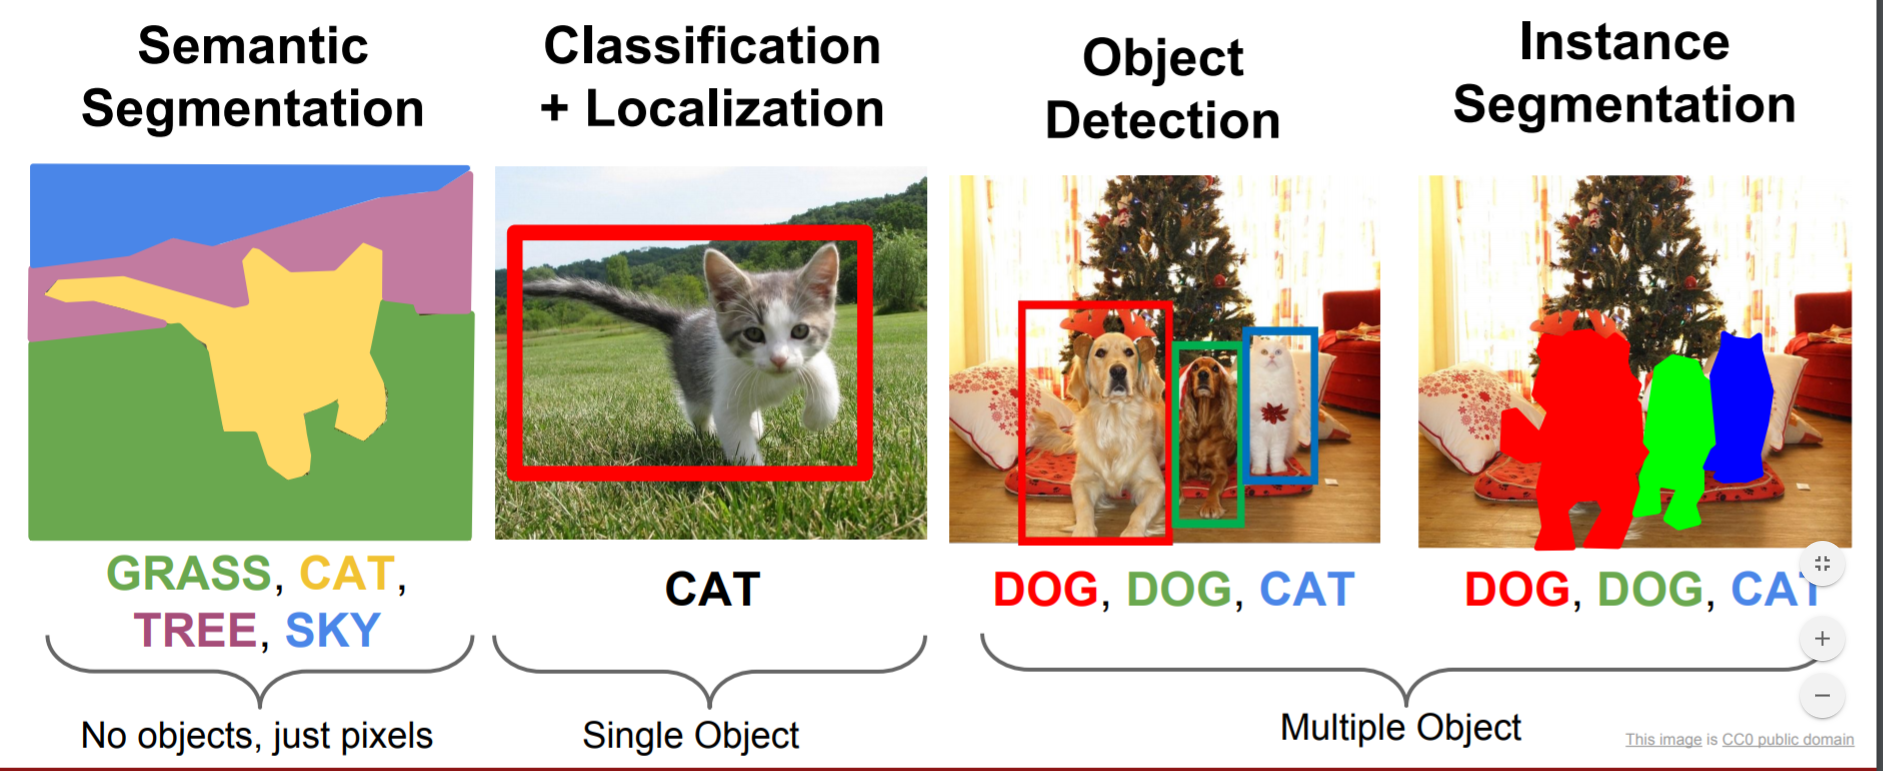
\includegraphics[width=\linewidth]{text/chapter_03/imgs/segmentation-types}
  \caption{Image detection and segmentation task types. (Source: \href{https://techvidvan.com/tutorials/image-segmentation-machine-learning/}{techvidvan.com}.)}
  \label{fig:seg_type}
\end{figure}

The development of object detection algorithms has evolved significantly over the years, driven by advances in deep
learning, dataset availability and computational power. Traditional object detection methods relied on handcrafted
features and machine learning algorithms, such as sliding window-based classifiers, histogram of oriented gradients (HOG) \cite{HoOGDalal2005}, and Haar cascades \cite{HaarCascadesLi2016}. While effective in certain scenarios, these methods often lacked robustness and scalability, particularly in complex and cluttered scenes.

With the advent of deep learning, convolutional neural networks (CNNs) improved the field of object detection. CNNs are
capable of automatically learning hierarchical representations of data, making them well suited for image analysis
tasks. The rise of CNN-based approaches has led to significant improvements in object detection accuracy and efficiency.
At its core, a convolutional neural network is comprised of multiple layers, each designed to perform specific operations on input data, typically images. The fundamental layers in a CNN include convolutional layers, pooling layers, and fully connected layers.
\begin{enumerate}
  \item \textbf{Convolutional layers:} These layers are responsible for extracting features from the input data. They consist of filters (also called kernels) that slide across the input image, performing a mathematical operation known as convolution. Each filter detects certain patterns or features, such as edges, textures, or shapes. By convolving the filters with the input image, the CNN can capture hierarchical representations of features, starting from simple edges and gradients to more complex structures.
  \item \textbf{Pooling layers:} Pooling layers are interspersed between convolutional layers to reduce the spatial dimensions of the feature maps while retaining important information. Common pooling operations include max pooling and average pooling, which downsample the feature maps by taking the maximum or average value within each pooling region. This downsampling helps in reducing computational complexity and controlling overfitting by enforcing spatial invariance.
  \item \textbf{Fully connected layers:} These layers are typically placed at the end of the CNN and serve to classify the features extracted by the convolutional layers. Each neuron in a fully connected layer is connected to every activation in the previous layer, forming a dense network. These layers use techniques like softmax activation to produce probability distributions over the classes in a classification task or regression outputs in a regression task.
\end{enumerate}
It is important to note, that it is common to combine more convolutional, pooling and fully connected layers with differently sized kernels in the architecture to improve the performance. Example of such architecture is shown in Figure \ref{fig:CNNArchitecture}
\begin{figure}
  \centering
  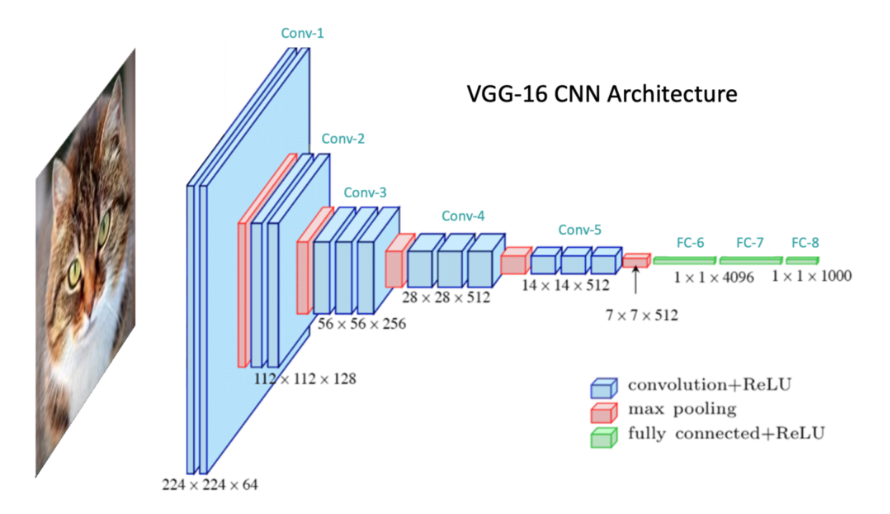
\includegraphics[width=\linewidth]{text/chapter_03/imgs/CNN}
  \caption{CNN architecture example. (Source \href{https://learnopencv.com/understanding-convolutional-neural-networks-cnn/}{learnopencv.com})}
  \label{fig:CNNArchitecture}
\end{figure}
During training, CNNs use a process called backpropagation to adjust the parameters (weights and biases) of the network based on the disparity between the predicted outputs and the ground truth labels. This optimization process aims to minimize a predefined loss function, such as cross-entropy loss for classification tasks or mean squared error for regression tasks. By iteratively updating the parameters using optimization algorithms like stochastic gradient descent (SGD) or its variants, CNNs gradually learn to recognize and classify patterns within the input data, ultimately improving their performance on various visual tasks such as object detection and segmentation.


Object detection poses several challenges, including variations in object appearance, scale, orientation, occlusion, and cluttered backgrounds. Additionally, real-world images often contain multiple objects of different classes, making it essential for detection algorithms to handle overlapping and partially visible objects.

Furthermore, object detection systems often have to balance accuracy and speed to meet the demands of real-time
applications. Achieving high detection accuracy while maintaining fast inference times is a fundamental challenge,
especially for devices with low hardware resources and applications requiring low-latency processing.

Object detection algorithms typically consist of several components:

\begin{itemize}
  \item \textbf{Input processing:} Images or video frames are preprocessed to standardize their format and size, often
involving resizing, normalization, and data augmentation to enhance model generalization.
  \item \textbf{Feature extraction:} Feature extraction is performed to capture relevant information from the input
  data. In deep learning-based approaches, convolutional neural networks are commonly used to extract hierarchical features that encode object appearance and spatial relationships.
  \item \textbf{Localization:} Localization involves predicting the spatial extent of objects within the image using
bounding boxes. This step requires regression or classification to estimate bounding box coordinates and confidence scores for object presence.
  \item \textbf{Classification:} Object classification assigns class labels to detected objects based on their visual
  appearance. Classification models are trained to distinguish between different object categories, enabling accurate identification of objects within the scene.
  \item \textbf{Post-processing:} Post-processing techniques, such as non-maximum suppression (NMS), are applied to
  refine detection results, suppress duplicate detections, and improve localization accuracy.
\end{itemize}



  \subsection{YOLO}

In the realm of object detection, the emergence of You Only Look Once (YOLO) represents a paradigm shift, propelled by the fusion of deep learning and innovative architectural design. YOLO stands as a testament to the transformative power of convolutional neural networks (CNNs) in redefining the landscape of computer vision applications, particularly in real-time object detection scenarios. This object detector was proposed by Developed by Joseph Redmon, Santosh Divvala, Ross Girshick, and Ali Farhadi in \cite{YOLORedmon2016}.

At its core, YOLO introduces a groundbreaking concept: the ability to predict bounding boxes and class probabilities for objects within an image in a single pass through the neural network. This departure from traditional object detection methods, which often involve multi-stage processes and post-processing steps, marks a significant leap forward in efficiency and speed. By consolidating object localization and classification into a unified framework, YOLO streamlines the detection pipeline, enabling seamless integration into various applications requiring rapid decision-making based on visual data.


A distinguishing feature of YOLO lies in its holistic approach to image analysis. Unlike conventional methods that segment images into regions of interest for further processing, YOLO takes a global perspective by dividing the input image into a grid and processing it as a whole. This global context consideration not only enhances the model's understanding of spatial relationships but also reduces the risk of misclassification, particularly in complex scenes with multiple objects. Each bounding box prediction includes coordinates $(x, y)$ for the center of the box, width, height, and confidence score indicating the likelihood of containing an object. Additionally, class probabilities are estimated for each bounding box to determine the object category. YOLO employs a loss function that penalizes localization errors, confidence errors, and classification errors.
This loss function is optimized during training using labeled datasets to learn accurate object representations. Moreover, YOLO adopts anchor boxes to improve localization accuracy and handle scale variations of objects within the image.

The evolution of YOLO over successive versions underscores its adaptability to diverse use cases and computational environments. While early iterations prioritized speed, subsequent iterations like YOLOv4 and YOLOv5 have aimed to enhance accuracy without compromising real-time performance \cite{YoloVersions2022}. This flexibility in model selection empowers users to tailor YOLO to their specific requirements, whether it be for surveillance systems demanding rapid detection or autonomous vehicles requiring precise object localization.

Compared to traditional object detection methodologies such as region-based convolutional neural networks (R-CNN) \cite{MaskRCNN2017} and single-shot detectors (SSD), YOLO stands out for its simplicity and efficiency. By eliminating the need for complex post-processing steps and leveraging a unified architecture for object detection (see Figure \ref{fig:yoloArchitecture} for YOLO architecture), YOLO achieves a fine balance between speed and accuracy. This versatility extends YOLO's applicability across a myriad of domains, including but not limited to autonomous driving, industrial automation, healthcare imaging, and augmented reality.

\begin{figure}
  \centering
  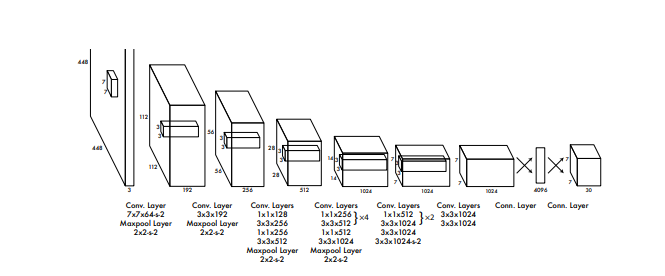
\includegraphics[width=\linewidth]{text/chapter_03/imgs/YOLO_architecture}
  \caption{Yolo architecture proposed in \cite{YOLORedmon2016} has 24 convolutinal layers followed by 2 fully connected layers. Convolutional layers were pretrained on the ImageNet classificator at half resolution (224 x 224 input image) and the doubled the resolution for detection. (Source \cite{YOLORedmon2016}.)}
  \label{fig:yoloArchitecture}
\end{figure}


\section{Image segmentation}
Image segmentation, a fundamental technique in computer vision, involves dividing a digital image into distinct pixel groups called segments. By breaking down the visual data into manageable segments, image segmentation facilitates more efficient and sophisticated image processing.

The methods employed for image segmentation vary from straightforward heuristic approaches to cutting-edge deep learning techniques. Traditional algorithms typically analyze basic visual attributes such as color and brightness to delineate object boundaries and background regions. Machine learning plays a pivotal role in this domain by training models on labeled datasets, allowing them to accurately classify objects and regions within images.

With its versatility and practical applications, image segmentation finds widespread use across artificial intelligence scenarios. Its applications span from assisting medical diagnoses through imaging to enabling automation in robotics and self-driving vehicles. Furthermore, it plays a crucial role in tasks such as identifying objects within satellite imagery.

There are three main task types in image segmentation: semantic segmentation, instance segmentation and panoptic segmentation \cite{IBM}.
The distinction between various types of image segmentation tasks hinges on how they handle semantic classes, which are specific categories assigned to individual pixels within an image.

In the realm of computer vision, semantic classes are broadly categorized into two types, each requiring distinct segmentation techniques for accurate results.
\begin{itemize}
  \item \textit{Things} represent classes of objects characterized by identifiable shapes, such as \textit{car, tree,} or \textit{person}. These classes typically consist of discrete instances with consistent sizes and distinguishable constituent parts. For instance, all cars have wheels, which are distinct from the car itself.
  \item \textit{Stuff} refers to semantic classes with amorphous shapes and variable sizes, like sky, water, or grass
  . Unlike \textit{things}, \textit{stuff} lacks clearly defined, countable individual instances and does not possess distinct parts. For example, both a single blade of grass and an entire field of grass fall under the category of \textit{grass}.
\end{itemize}
In certain image contexts, some classes can straddle the line between being considered \textit{things} or \textit{stuff}. For instance, a large gathering of people might be interpreted either as multiple people -- each being a clearly shaped, countable thing, or as a singular, indistinct person.

While much of the focus in object detection typically centers on \textit{thing} classes, it is crucial to recognize that \textit{stuff}, such as sky, walls, floors, and ground constitutes the bulk of our visual environment. \textit{Stuff} serves as crucial contextual information for identifying \textit{things}. For instance, a metallic object on the road is likely a car, while a blue background behind an object is indicative of water if it is a boat or sky if it is a plane. This interplay between \textit{stuff} and \textit{things} holds particular significance for deep learning models.

  \subsection{Semantic segmentation}
Semantic segmentation represents the most straightforward form of image segmentation. In this approach, a semantic segmentation model assigns a semantic class to every pixel in an image, without providing additional context or information, such as the identification of specific objects.

Unlike more nuanced segmentation techniques, semantic segmentation treats all pixels uniformly as \textit{stuff} without distinguishing between \textit{stuff} and \textit{things}. This means that it does not differentiate between different types of objects within the same class.

For instance, imagine a semantic segmentation model trained to analyze urban scenes. It would generate segmentation masks outlining the boundaries of various classes of \textit{things} and \textit{stuff}. However, it would not differentiate between individual instances of the same class. For example, if there are multiple trees in a forest, the model would likely treat them as one continuous tree segment rather than recognizing each individual tree separately.

\subsection{Instance segmentation}
Instance segmentation represents a departure from the approach of semantic segmentation. While semantic segmentation focuses solely on assigning semantic classes to each pixel without distinguishing between individual instances, instance segmentation precisely outlines the shape of each separate object instance within an image.

In essence, instance segmentation segregates \textit{things} from \textit{stuff}, disregarding the latter, and can be viewed as a more sophisticated version of object detection. Instead of providing rough bounding boxes, instance segmentation furnishes precise segmentation masks for each object instance.

This task poses greater challenges compared to semantic segmentation. Even when instances of the same class overlap or touch each other, instance segmentation models must accurately separate and delineate the shape of each instance. In contrast, semantic segmentation models may simply group them together.

Instance segmentation algorithms typically adopt either a two-stage or one-shot methodology to address the task.

Two-stage models, exemplified by Region-based Convolutional Neural Networks \cite{RCNN2014}, initially conduct conventional object detection to produce bounding boxes for each potential instance. Subsequently, they refine segmentation and classification within these bounding boxes to precisely delineate each object instance.

Conversely, one-shot models, such as YOLO, streamline the process by simultaneously performing object detection, classification, and segmentation. This approach enables real-time instance segmentation.

While one-shot methods boast faster processing speeds, they often sacrifice some accuracy. On the other hand, two-stage approaches prioritize accuracy but may be slower due to the additional refinement steps.

  \subsection{Panoptic segmentation}
Panoptic segmentation represents a synthesis of semantic and instance segmentation methodologies, offering a comprehensive understanding of an image.

In panoptic segmentation, each pixel receives both a semantic label and an instance ID. Pixels with the same label and ID are assigned to the same object instance. For \textit{stuff} pixels, the instance ID is disregarded.

This approach provides computer vision systems with a complete and cohesive interpretation of an image, combining the benefits of both semantic and instance segmentation. However, achieving panoptic segmentation consistently and efficiently presents significant computational challenges. Despite its evident appeal, realizing panoptic segmentation in a manner that balances accuracy and computational efficiency remains a formidable task.

The challenge in achieving panoptic segmentation lies in reconciling the conflicting approaches of semantic and instance segmentation models. Semantic segmentation treats all pixels uniformly as \textit{stuff}, disregarding individual instances of objects, while instance segmentation focuses solely on isolating individual objects, ignoring \textit{stuff}. Integrating these methodologies proves difficult as neither model can effectively take on the responsibilities of the other.

Early attempts at panoptic segmentation involved combining separate semantic and instance segmentation models, followed by a post-processing phase to merge their outputs. However, this approach encountered two significant drawbacks: it demanded substantial computational resources and struggled with inconsistencies between the data produced by the semantic segmentation network and that produced by the instance segmentation network.

Recent advancements in panoptic segmentation architectures aim to overcome these limitations through a more unified deep learning approach. Many of these architectures utilize a common backbone network, such as a feature pyramid network (FPN) \cite{FPNLin2017}, to extract features from the input image. These features are then fed into parallel branches, such as a foreground branch and a background branch, or a semantic head and an instance head. The outputs from each branch are merged using a weighted system to produce the final segmentation. Notable proposed architectures include EfficientPS \cite{mohan2020efficientps}, OANet \cite{zhang2019oanet}, PanopticFPN \cite{kirillov2019panoptic}, UPSNet \cite{xiong2019upsnet}, SOGNet \cite{yang2019sognet}, BGRNet \cite{wu2020bidirectional}, AUNet \cite{sun2019aunet} and others.

\subsection{Traditional image segmentation}
Traditional image segmentation techniques leverage pixel color values and related characteristics, such as brightness, contrast, or intensity, for feature extraction. These methods are often trained with simple machine learning algorithms and are particularly useful for tasks like semantic classification. Despite their limitations in precision compared to deep learning-based approaches, traditional methods offer advantages in terms of lower cost and computational demands, allowing them to efficiently solve certain problems.

Some common traditional image segmentation techniques include:
\begin{enumerate}
  \item \textbf{Thresholding:} Thresholding methods create binary images by classifying pixels based on whether their intensity exceeds or falls below a predetermined threshold value. Otsu's method is frequently used to identify the threshold value that minimizes intra-class variation \cite{otsu1979}.
  \item \textbf{Histograms:} Histograms plot the frequency of specific pixel values in an image and are often employed to define thresholds. For instance, histograms can infer background pixel values, aiding in the isolation of object pixels.
  \item \textbf{Edge detection:} Edge detection techniques identify object boundaries or classes by detecting abrupt changes in brightness or contrast \cite{Edgedet1986}.
  \item \textbf{Watersheds:} Watershed algorithms \cite{Watershed1991} convert images to grayscale and generate a topographic map where each pixel's elevation is determined by its brightness. Regions, boundaries, and objects can be inferred from the formation of valleys, ridges, and catchment basins.
  \item \textbf{Region-based segmentation:} Region-growing algorithms \cite{RCNN2016} initiate segmentation with one or more seed pixels, progressively grouping neighboring pixels with similar characteristics. These algorithms can be either agglomerative or divisive.
  \item \textbf{Clustering-based segmentation:} Clustering algorithms \cite{ClusteringSeg1979}, an unsupervised learning technique, partition visual data into clusters of pixels with similar values. One popular variant is K-means clustering, where k represents the number of clusters. In this method, pixel values are treated as data points, and $k$ random points are selected as the centroids of clusters. Each pixel is then assigned to the nearest centroid based on similarity. Centroids are iteratively relocated to the mean of each cluster until convergence, resulting in stabilized clusters.
\end{enumerate}

\subsection{Deep learning image segmentation}
Trained on meticulously annotated datasets, deep learning image segmentation models harness the power of neural networks to uncover underlying patterns within visual data. These models discern salient features crucial for tasks such as classification, detection, and segmentation.

Despite their higher computational requirements and longer training times, deep learning models consistently outperform traditional approaches, serving as the cornerstone for ongoing advancements in computer vision.

Some prominent deep learning models utilized in image segmentation include:

\begin{enumerate}
  \item \textbf{Fully Convolutional Networks:} FCNs \cite{FCNLong2015}, commonly employed for semantic segmentation, are a
  variant
  of
  convolutional neural networks characterized by flexible layers. In FCNs, an encoder network processes visual input through convolutional layers to extract pertinent features for segmentation or classification. The compressed feature data is then passed through decoder layers to upsample and reconstruct the input image along with segmentation masks.
  \item \textbf{U-Nets:} U-Nets \cite{ronneberger2015unet} adapt the FCN architecture to mitigate data loss during downsampling by
  incorporating skip connections. These connections enable the preservation of finer details by selectively bypassing
  certain convolutional layers as information propagates through the network. The name U-Net derives from the shape 
  of diagrams illustrating its layered arrangement (see Figure \ref{fig:unet_architecture}).
  \item \textbf{Deeplab:} Similar to U-Nets, Deeplab modifies the FCN architecture \cite{Deeplab2018}. In addition to utilizing skip
  connections, Deeplab employs dilated (or "atrous") convolution to produce larger output maps without requiring additional computational resources.
  \item \textbf{Mask R-CNNs:} Mask R-CNNs stand out as a leading model for instance segmentation \cite{MaskRCNN2017}. These models
  integrate a region proposal network (RPN), responsible for generating bounding boxes for potential instances, with an FCN-based "mask head" that produces segmentation masks within each confirmed bounding box.
  \item \textbf{Transformers:} Inspired by the success of transformer models \cite{vaswani2023attention} in natural language processing,
  newer models like the Vision Transformer (ViT) employ attention mechanisms in lieu of convolutional layers. These models have demonstrated comparable or superior performance to CNNs for various computer vision tasks.
\end{enumerate}

\begin{figure}
  \centering
  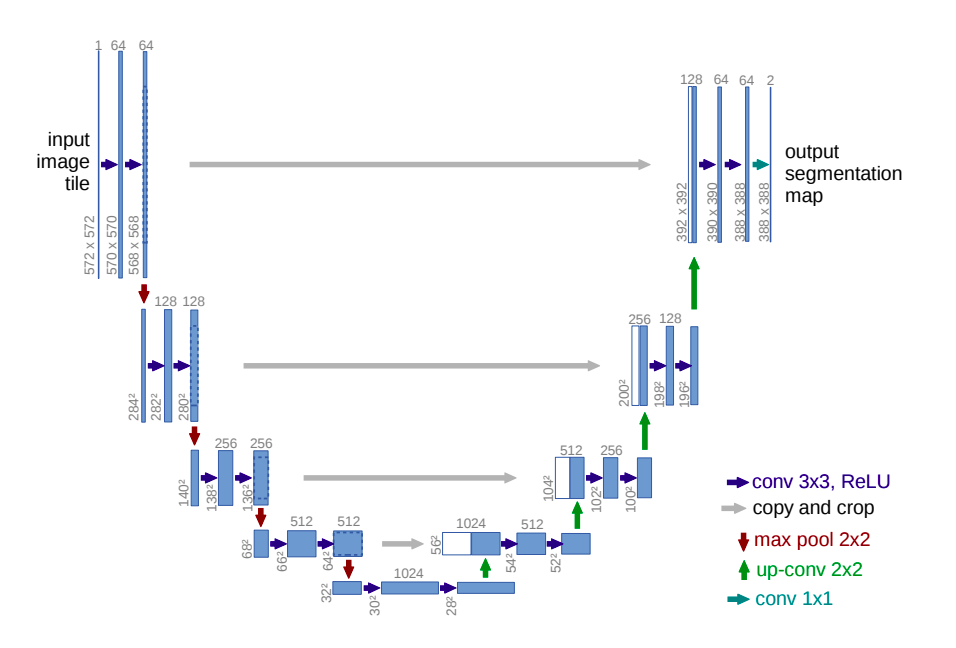
\includegraphics[width=\linewidth]{text/chapter_03/imgs/unet}
  \caption{U-net architecture (example for 32x32 pixels in the lowest resolution). (Source \cite{ronneberger2015unet})}
  \label{fig:unet_architecture}
\end{figure}

\subsubsection{Transformers}
As we use Transformer model in our work, we briefly demonstrate Transformers' architecture and how they work.
Transformers consist of a stack of identical layers, typically comprising an encoder and a decoder (Figure \ref{fig:transformer_architecture}). The
encoder
processes the input sequence, while the decoder generates the output sequence.


\begin{figure}
  \centering
  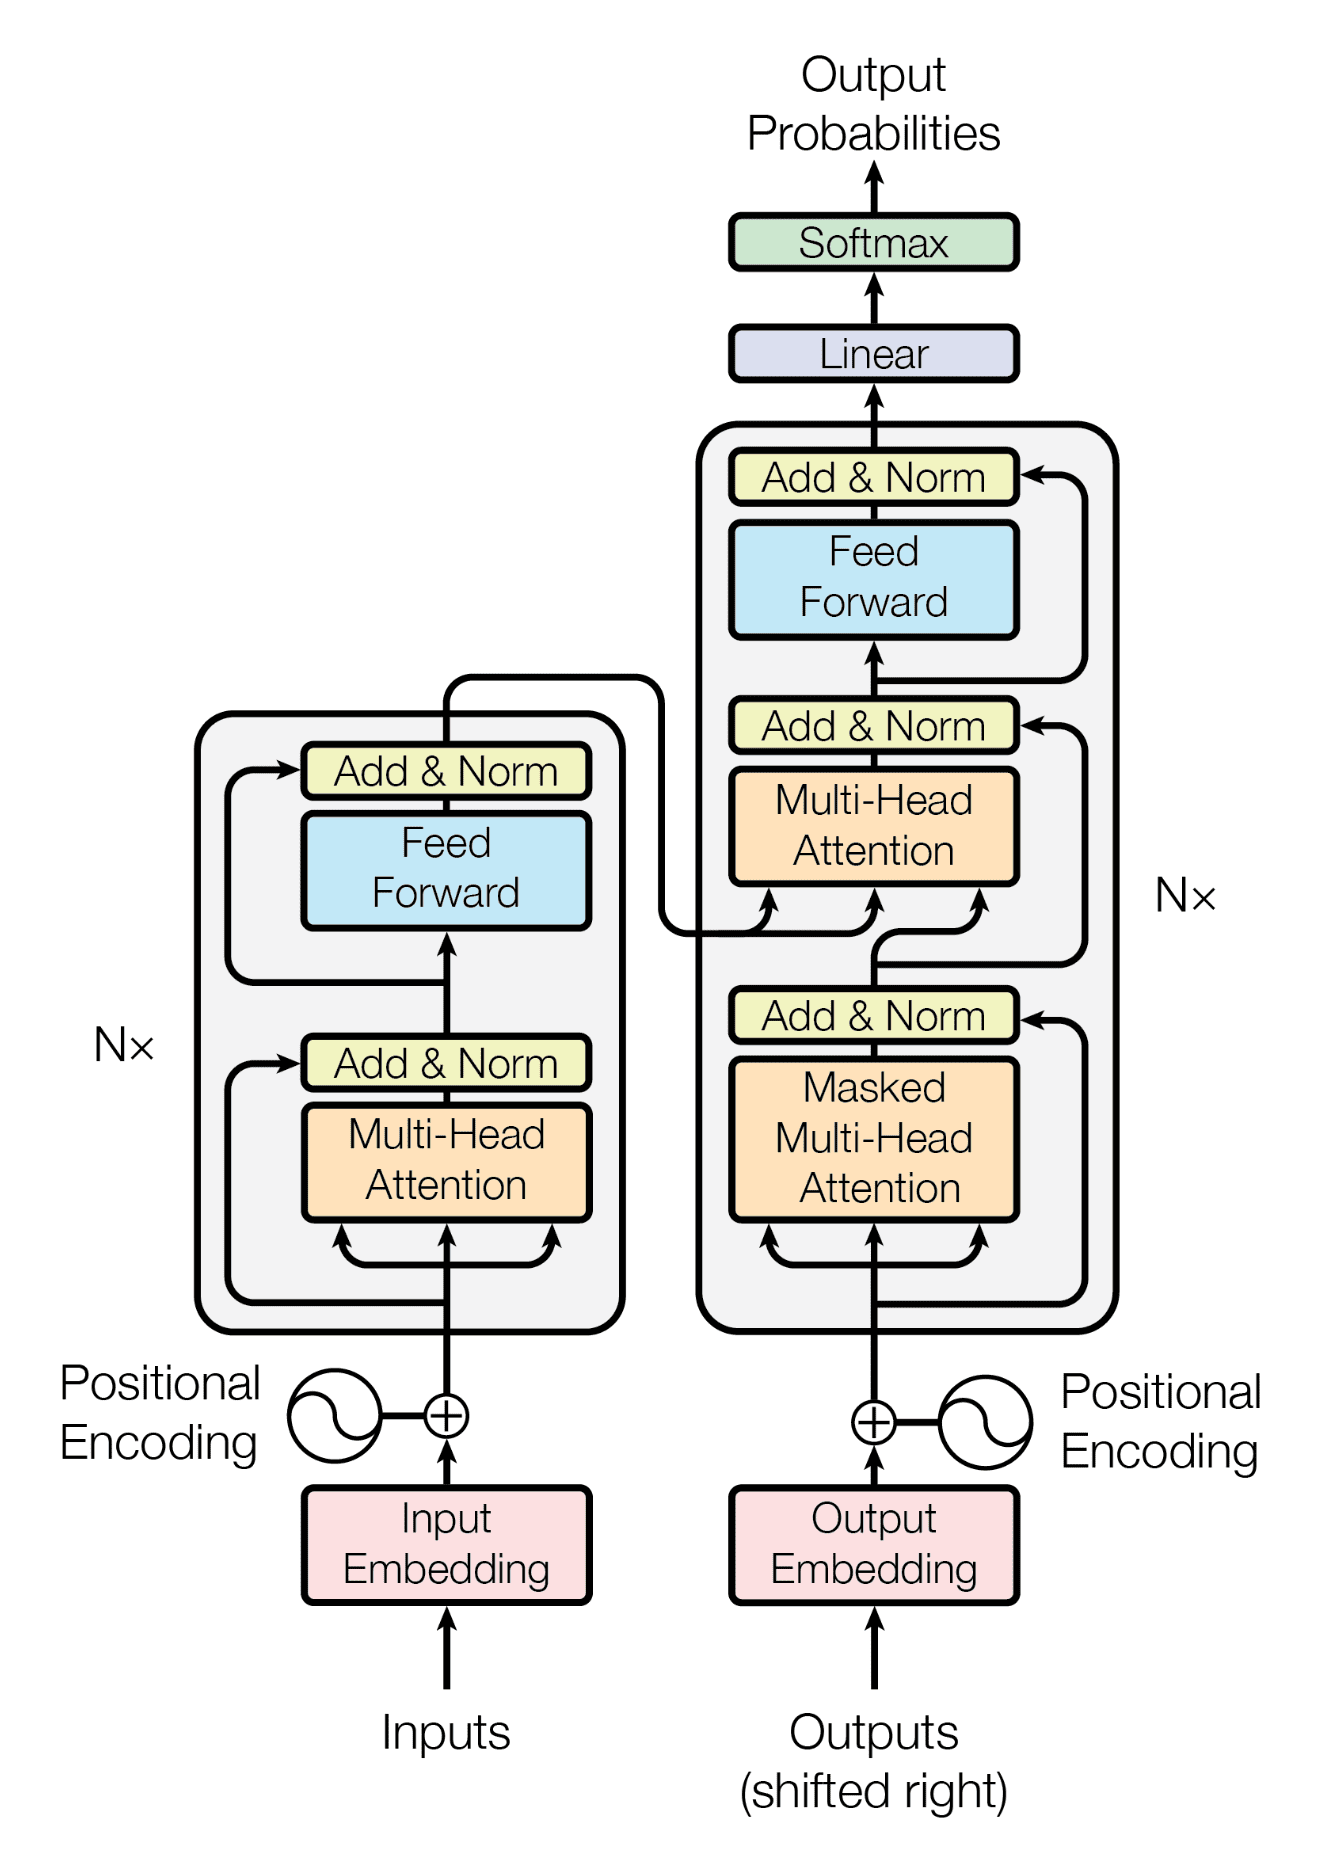
\includegraphics[width=0.5\linewidth]{text/chapter_03/imgs/transformers}
  \caption{Transformer architecture. (Source \cite{vaswani2023attention})}
  \label{fig:transformer_architecture}
\end{figure}

\begin{itemize}
  \item \textbf{Encoder:} The encoder is composed of a stack of $N=6$ identical layers. Each layer has two
  sub-layers. The first is a multi-head self-attention mechanism (Figure \ref{fig:transformer_multihead}), and the second is positionwise fully
  connected feed-forward network. There is a residual connection \cite{DeepResidual2016} around each of two sub-layers, followed by normalization \cite{ba2016layer}: the output of each sub-layer is $LayerNorm(x + Sublayer(x))$, where $Sublayer(x)$ is the function implemented by the sub-layer
  itself.
  \item \textbf{Decoder:} The decoder is also composed of a stack of $N=6$ identical layers. In addition to the two
  sub-layers in each encoder layer, the decoder inserts a third sub-layer, which performs multi-head
  attention over the output of the encoder stack. Similar to the encoder, there is residual connections
  around each of the sub-layers, followed by layer normalization.
\end{itemize}

\begin{figure}
  \centering
  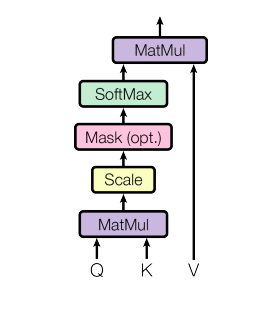
\includegraphics[width=0.5\linewidth]{text/chapter_03/imgs/multihead}
  \caption{Multi-head attention. (Source \cite{vaswani2023attention})}
  \label{fig:transformer_multihead}
\end{figure}


The core of the Transformer architecture lies in its self-attention mechanism \cite{vaswani2023attention}. This mechanism enables each token in the input sequence to attend to every other token, learning contextual relationships and dependencies. By computing attention scores between all pairs of tokens and taking weighted sums of their embeddings, the Transformer can effectively capture long-range dependencies and dependencies between distant tokens.

To enhance the expressiveness of self-attention, Transformers employ multi-head attention mechanisms. Instead of computing attention once, multi-head attention computes attention multiple times in parallel, each with its set of learnable parameters. This allows the model to attend to different aspects of the input sequence simultaneously, facilitating richer representations and improved performance.

Unlike sequential models, Transformers do not inherently encode the positional information of tokens. To address this limitation, positional encoding is added to the input embeddings to convey the position of each token in the sequence. This positional information is crucial for the Transformer to distinguish between tokens with the same content but different positions within the sequence.

In addition to self-attention layers, Transformers incorporate feedforward neural networks within each layer. These FNNs consist of multiple fully connected layers with non-linear activation functions, enabling the model to capture complex interactions and transformations within the input data
\begin{align}
  FFN(x) &= max(0, xW_1 + b_1)W_2 + b_2,
\end{align}
where $W$ are weights and $b$ stands for bias.

To stabilize training and facilitate gradient flow, Transformers employ layer normalization and residual connections within each layer. Layer normalization normalizes the activations across feature dimensions, while residual connections enable the direct flow of gradients through the network, mitigating the vanishing gradient problem.

During training, Transformers are optimized using backpropagation and gradient-based optimization algorithms, such as
Adam \cite{kingma2017adam} or SGD \cite{rakhlin2012making}, to minimize a predefined loss function. By iteratively updating the
parameters of the model based on
the disparity between the predicted outputs and the ground truth labels, Transformers learn to encode and generate
meaningful representations of input sequences, enabling them to excel in various NLP tasks and more recently
image processing tasks.



%Object segmentation involves partitioning an image into semantically meaningful regions and associating each region with a specific object instance. Unlike object detection, which identifies objects at the bounding box level, segmentation provides pixel-level delineation of object boundaries. This fine-grained information is invaluable for tasks such as image understanding, scene understanding and image manipulation.

%Semantic segmentation assigns a class label to each pixel in the image, effectively partitioning the image into regions corresponding to different object categories. Fully Convolutional Networks (FCNs) and their variants, such as U-Net and DeepLab, have demonstrated remarkable success in semantic segmentation tasks by leveraging the power of convolutional neural networks for dense pixel-wise predictions \cite{SemanticSegmentationGuo2022}.

%Instance segmentation, on the other hand, extends semantic segmentation by distinguishing between individual object instances of the same class. This task requires not only segmenting objects but also differentiating between instances of the same class, even if they overlap or occlude each other. Mask R-CNN, an extension of Faster R-CNN, combines region-based object detection with instance segmentation, achieving state-of-the-art results in both tasks.

%Despite significant advancements, object detection and segmentation still face several challenges. These include handling scale variations, occlusions, cluttered backgrounds, and fine-grained object attributes. Additionally, achieving real-time performance while maintaining high accuracy remains a critical goal for many applications.

  \subsection{Segment anything}
To get the best possible results in practical part of this thesis, it is necessary to use powerful, yet fast image
segmentation model. The Segment Anything (SAM) model represents a significant advancement in image segmentation,
introducing a novel approach to tackling the challenges in this field \cite{SAM2023}. SAM is designed to address the need for
efficient and effective segmentation models that can generalize to diverse tasks and data distributions, even in zero-shot scenarios.

The SAM project introduces a new task, model, and dataset for image segmentation. It leverages a promptable model
architecture to achieve impressive zero-shot performance on diverse segmentation tasks. This task involves generating valid segmentation masks given any segmentation prompt. A prompt can include spatial or textual information indicating what to segment in an image. SAM ensures the output mask is reasonable for at least one interpretation of the prompt, handling ambiguity effectively.

SAM's architecture comprises three main components: an image encoder, a prompt encoder, and a mask decoder (Figure \ref{fig:sam_architecture}). The
image encoder processes input images using a Vision Transformer, while the prompt encoder handles various types of prompts, including points, boxes, and text. The mask decoder efficiently generates segmentation masks based on the input image and prompt embeddings. SAM is designed for real-time performance, enabling interactive use with low latency.

\begin{figure}[h]
  \centering
  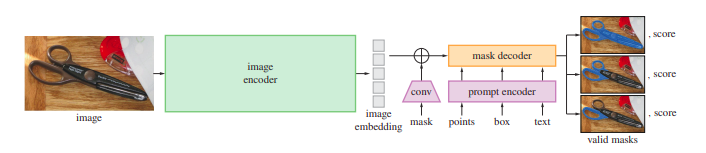
\includegraphics[width=\linewidth]{text/chapter_03/imgs/sam}
  \caption{SAM architecture (Source \cite{SAM2023})}
  \label{fig:sam_architecture}
\end{figure}

SAM addresses ambiguity by predicting multiple output masks for a single prompt. It efficiently ranks these masks based on confidence scores, allowing it to produce accurate segmentations even in complex scenarios.

Efficiency is a core consideration in SAM's design. The model's components are optimized for fast execution, enabling it to run in a web browser on CPU with a runtime of approximately 50ms. This real-time performance facilitates seamless interaction with the model for prompt-based segmentation tasks.

SAM is trained using the linear combination of focal loss \cite{FocalLoss2020} and dice loss \cite{DiceLoss2016}, tailored for the
promptable segmentation
task. It simulates an interactive setup during training, sampling prompts to ensure robustness and adaptability.

SAM's contributions include the development of a promptable segmentation task, a novel model architecture optimized
for real-time performance, and a large-scale dataset (SA-1B) comprising over 1 billion masks and 11 million images.
The model's zero-shot capabilities and efficient design make it a valuable tool for various segmentation tasks, with
potential applications across diverse domains. The example of segmented images are shown in Figure \ref{fig:sam_example}.

\begin{figure}[h]
  \centering
  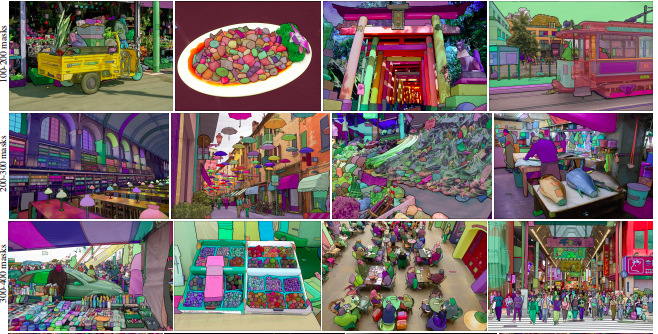
\includegraphics[width=\linewidth]{text/chapter_03/imgs/sam_example}
  \caption{The demonstration of SAM's strength. These masks were annotated fully automatically by SAM and are part of
  the SA-1B dataset. (Source \cite{SAM2023})}
  \label{fig:sam_example}
\end{figure}

\subsection{Grounded segment anything}
As SAM text prompt was not released yet,\ldots
\todo{try it}

\chapter{Dynamic time and state varying detection probability}
As stated in the Introduction, this work focuses on tracking objects in frame sequence using target tracking methods
and
object detection
and
segmentation algorithms. Object detectors, which were discussed in the previous section, are essential for getting
measurements
from an image.

Note, that in all target tracking algorithms for cluttered environments and targets
birth and dead possibilities, there is a parameter called the detection probability ($p_D$). As its name
suggests, this parameter expresses a probability that the target is detected in the particular time. It is also commonly
used
as a
time- and state-independent scalar. The desired outcome is to enhance the performance of multi-target
algorithms
in video data
in scenarios, where the targets may be hidden by an obstacle, and reduce impacts of a misdetection of a sensor.
Therefore, it
is appropriate to have a dynamic time- and state-varying detection probability.
\section{Problem definition}
\label{sec:mphd_problemDef}
In the practical part of this thesis, three different settings of object detection and segmentation can be found.
We choose Probability Hypothesis Density filter as a multi-target tracking algorithm, as it is a simpler
RFS-based method. PHD filter is computationally very effective in comparison with filters such as the CPHD or the
PMBM filter,
which may seem as a more appropriate option for this task. However, these more complicated filters have high
computational demands, which
are not adequate when used in video streams. Provided settings are:
\begin{enumerate}
  \item \textbf{S1: YOLO + PHD} -- Yolo itself can produce an object segmentation mask with lower accuracy, but with
  greater
  speed. This setting is suitable when using CPU only.
  \item \textbf{S2: YOLO + SAM + PHD} -- As SAM cannot annotate labels to objects, it requires another object detector
  before segmentation. In this setting, we use YOLO as an object detector and SAM for mask segmentation of detected
  objects. This procedure requires GPU for faster computation.
  \item \textbf{S3: Grounded SAM + PHD} -- Grounded SAM is the most universal approach, as it can detect objects based
  on a text input and uses SAM for segmentation. This setting also requires GPU for faster computation.
\end{enumerate}


\subsection{The modified GM-PHD filter}
To modify the GM-PHD filter for our use case, a few assumptions have to be introduced. These assumptions are very
similar to the ones of the PHD filter and the GM-PHD filter in Section \ref{sec:phdfilter} and \ref{sec:gmphdFilter}.
\begin{enumerate}
  \item Each target evolves and generates observations independently of each other. \label{as:mphd_1}
  \item Clutter is Poisson and independent of target-originated measurements. \label{as:mphd_2}
  \item The predicted multi-target RFS governed by $p_{k|k-1}$ is Poisson. \label{as:mphd_3}
  \item Each target follows a linear Gaussian dynamical model and the sensor has a linear \label{as:mphd_4}
  Gaussian measurement model, i.e.,
  \begin{align}
    f_{k|k-1}(x|\xi) &= \mathcal{N}(x; F_{k-1}\xi, Q_{k-1}),\\
    g_k(z|x) &= \mathcal{N}(z;H_kx, R_k),
  \end{align}
  where $\mathcal{N}(\cdot;\cdot,\cdot)$ is a Gaussian density, $Q_{k-1}$ is the process noise covariance, $H_k$ is the observation matrix and $R_k$ is the observation noise covariance.
  \item The survival probability is state-independent, i.e.,
  \begin{align}
    p_{S,k}(x) &= p_{S,k}.
  \end{align}
    \label{as:mphd_5}
  \item The detection probability is state-dependent, i.e.,
    \begin{align}
      p_{D,k}(x) &= 
      \begin{cases}
         p_{D,k} &\qquad \text{if detected for the first time,} \\
         p_{D,k}(x) &\qquad \text{otherwise.}
      \end{cases}
    \end{align}
    \label{as:mphd_6}
  \item The intensity of the birth RFS is a Gaussian mixture of the form
  \begin{align}
    \gamma_k(x) &= \sum_{i=1}^{J_{\gamma,k}}w_{\gamma,k}^{(i)} \mathcal{N}\left(x; m_{\gamma.k}^{(i)}, P_{\gamma,k}^{(i
    )}\right).
    \label{eq:mphd_intensity}
  \end{align}
  \label{as:mphd_7}
\end{enumerate}
Note, that the assumption \ref{as:mphd_1} may be questionable, as the states of each of the targets are often
dependently
evolving.
Imagine,
for example, a common traffic scenario. If one of the cars immediatelly stops, the following vehicles have to stop as
well. Meaning, they are affected by another target.
The assumption \ref{as:mphd_2} is reasonable, especially if we consider that the clutter rate should be very low in
our
scenarios.
The survival probability is state-independent as in the GM-PHD filter and should be set high, as the targets are
expected
to survive to the next time step.
The detection probability is state-dependent and equal to $p_{D,k}$, i.e., a predefined threshold, in situation when
the target is detected for the first time. Otherwise, if the target has evolved from the previous state $\xi$, the
detection probability is calculated according to Section \ref{sec:dynamic_pd}.
Assumption \ref{as:mphd_7} contains only intensity of the birth RFS, the spawn intensity RFS is left out.
Nevertheless, it still can be easily added to the assumption
and equations afterwards.

\subsubsection{The modified PHD recursions}
Let us assume a target state $x$ described by an intensity function $\nu(x)$. At time $k$, the prediction of the prior
intensity $\nu_{k-1}(x)$ is given by
\begin{equation}
  \nu_{k|k-1}(x) = \int p_{S,k}(\xi)\phi_{k|k-1}(x|\xi)\nu_{k-1}(\xi)d\xi + \nu_{\gamma,k}(x), \label{eq:mphdPrior}
\end{equation}
where $p_{S,k}(\cdot)$ is the probability of target survival, $\phi_{k|k-1}(\cdot|\cdot)$ is the target state transition density, and $\nu_{\gamma,k}(\cdot)$ denotes the prior PHD of the targets birth at time k.
The predicted intensity $\nu_{k|k-1}$ is then updated by the measurement set $Z_k$ given by sensors at time $k$ according to the Bayesian update
\begin{equation}
  \begin{aligned}
    \nu_k(x) &= [1 - p_{D,k}(x)]\nu_{k|k-1}(x) \\
    &+ \sum_{z \in Z_k}\frac{p_{D,k}(x) g_k(z|x) \nu_{k|k-1}(x)}{\kappa_k(z) + \int p_{D,k}(\xi) g_k(z|\xi) \nu_{k|
    k-1}(\xi)d\xi}, \label{eq:mphdPosterior}
  \end{aligned}
\end{equation}
where $g_k(\cdot|\cdot)$ is the likelihood function, $p_{D,k}(\cdot)$ is the probability of detection, and $\kappa_k(\cdot)$ is the clutter density.

\subsubsection{The modified GM-PHD recursion}
\label{sec:mGMPHDrec}
In the context of the linear Gaussian multiple-target model, the PHD recursion equations (\ref{eq:mphdPrior}) and (\ref{eq:mphdPosterior}) attain analytical solution \cite{VoMaPHD2006}.
Suppose that the posterior intensity at time $k-1$ is a Gaussian mixture of the form
\begin{equation}
  \label{eq:mphd_recursion_posterior}
  \begin{aligned}
    \nu(x) &= \sum_{i=1}^{J_{\gamma,k}} w_{\gamma,k}^{(i)}\mathcal{N}(x;m_{\gamma,k}^{(i)},P_{\gamma,k}^{(i)}).
  \end{aligned}
\end{equation}
The predicted intensity for time $k$ is also a Gaussian mixture of the form
\begin{equation}
  \label{eq:mphd_recursion_prior}
  \begin{aligned}
    \nu_{k|k-1}(x) &= \nu_{S,k|k-1}(x) + \gamma_k(x),
  \end{aligned}
\end{equation}
where $\gamma_k(x)$ is given in Formula (\ref{eq:mphd_intensity}). This yields
\begin{align}
  \nu_{S,k|k-1}(x) &= p_{S,k}\sum_{j=1}^{J_{k-1}}w_{k-1}^{(j)} \mathcal{N}(x;m_{S,k|k-1}^{(j)}, P_{S,k|k-1}^{(j)}) \label{eq:mphd_recursion_predict_intensity}, \\
  m_{S,k|k-1}^{(j)} &= F_{k-1}m_{k-1}^{(j)},  \label{eq:mphd_recursion_predict_m} \\
  P_{S,k|k-1}^{(j)} &= Q_{k-1} + F_{k-1}P_{k-1}^{(j)}F_{k-1}^T.  \label{eq:mphd_recursion_predict_P}
\end{align}
Thus the predicted intensity at the time $k$ is a Gaussian mixture
\begin{align}
  \nu_{k|k-1}(x) &= \sum_{i=1}^{J_{k|k-1}}w_{k|k-1}^{(i)} \mathcal{N}(x;m_{k|k-1}^{(i)}, P_{k|k-1}^{(i)}),  \label{eq:mphd_recursion_predict_intesity}
\end{align}
and the posterior intensity at time $k$ is also Gaussian mixture,
\begin{align}
  \nu_{k}(x) &= \sum_{i=1}^{J_{k|k-1}}[1-p_{D,k}^{(i)}(x)]w_{k|k-1}^{(i)} \mathcal{N}(x;m_{k|k-1}^{(i)}, P_{k|k-1}^{(
  i)})\nonumber \\
  &+ \sum_{z\in Z_k}\nu_{D,k}(x;z), \label{eq:mphd_recursion_update_intesity}
\end{align}
where
\begin{align}
  \nu_{D,k}(x;z) &= \sum_{j=1}^{J_{k|k-1}} w_k^{(j)}(z) \mathcal{N}(x;m_{k|k}^{(j)}(z),P_{k|k}^{(j)}), \label{eq:mphd_recursion_update_intesity_detect} \\
  w_k^{(j)}(z) &= \frac{p_{D,k}^{(j)}(x;z) w_{k|k-1}^{(j)} q_k^{(j)}(z) }{\kappa_k(z) + p_{D,k}^{(j)}(x;z) \sum_{l=1}^{J_{k|k-1}} w_{k|k-1}^{(l)} q_k^{(l)}(z)}, \label{eq:mphd_recursion_update_intesity_detect_w} \\
  m_{k|k}^{(j)}(z) &= m_{k|k-1}^{(j)} + K_k^{(j)}(z-H_k m_{k|k-1}^{(j)}), \label{eq:mphd_recursion_update_intesity_detect_m} \\
  P_{k|k}^{(j)}(z) &= [I - K_k^{(j)} H_k] P_{k|k-1}^{(j)},  \label{eq:mphd_recursion_update_intesity_detect_P} \\
  \kappa_{k}^{(j)}(z) &= P_{k}^{(j)} H_k^T(H_k P_{k|k-1}^{(j)} H_k^T + R_k)^{-1}. \label{eq
  :mphd_recursion_update_intesity_detect_K}
\end{align}
The dynamically estimated detection probability in \eqref{eq:mphd_recursion_update_intesity} follows from one of two
possible scenarios described in Section \ref{sec:dynamic_pd}.
\subsection{S1: YOLO + PHD}
It is possible to fine-tune YOLO model on personalised datasets to either improve the performance in the
detection of
pretrained classes, or to train the model for detecting other classes. With over 70 pretrained class instances, it is
not necessary to fine tune our YOLO model for the experiments in this work. The model also detects all class
instances it is trained for, that appear in a scene. For testing purposes, we filter only objects we want to detect
and get
measurements from. The YOLO itself is able to produce a segmentation mask in real-time, but with less
accuracy
and
precision. This is caused by a reduced image resolution which is $640x640$ pixels. To fit the YOLO output
to our
frame,
this output needs to be resized back to our desired frame size. This resizing causes some imperfections. However, the
precision
to pixel level is not always necessary in our scenarios, thus this setting is, in most cases, sufficient
enough. The advantage of this approach is that it runs quickly enough with CPU only. The example of
object segmentation YOLO model is shown in the Figure \ref{fig:yolo_seg}.
\begin{figure}[h]
  \centering
  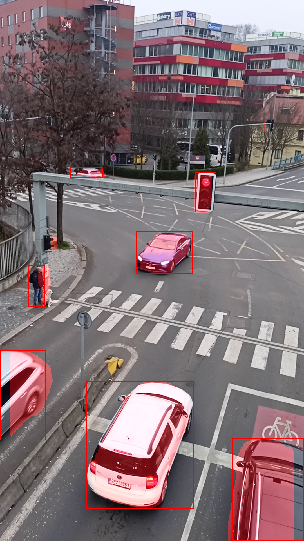
\includegraphics[width=0.35\linewidth]{text/chapter_04/imgs/YOLO_screenshot_2}
  \caption{YOLO segmentation example. This picture shows all detected objects the YOLO model is trained for and also
  the segmented objects' masks. These masks are imperfect, but often sufficient enough. This figure was taken in
  Kartouzská street, Prague.}
  \label{fig:yolo_seg}
\end{figure}

\subsection{S2: YOLO + SAM + PHD}
The SAM model architecture in \cite{SAM2023} is prepared to first process a text input and then segment objects based
on the
input. However, this feature is not available yet in the original implementation, and, for our purposes, we need an
object
detector before the segmentation process can be performed. The SAM model is able to segment a desired object based on
one
of two provided
inputs with high precision and accuracy. The first possible input is a bounding box around the required object, which
can be provided by an output of the YOLO model. The second option is to provide a rough center point of an object, which
can also be the center of a bounding box provided by the YOLO model.

However, for our purposes, it is not recommended
to use the combination of both inputs, as SAM is able to produce multiple masks for an object. For example, if we
denote, that we want to segment a whole person by a bounding box, one of the output masks can be just his jacket, as it
makes a
valid segmentation mask. Combining these two inputs can, therefore, produce this undesirable output. Another
example of
such
behaviour
is shown in the Figure \ref{fig:sam_examples}
\begin{figure}[htbp]
  \centering
  \begin{subfigure}[h]{0.48\textwidth}
    \centering
    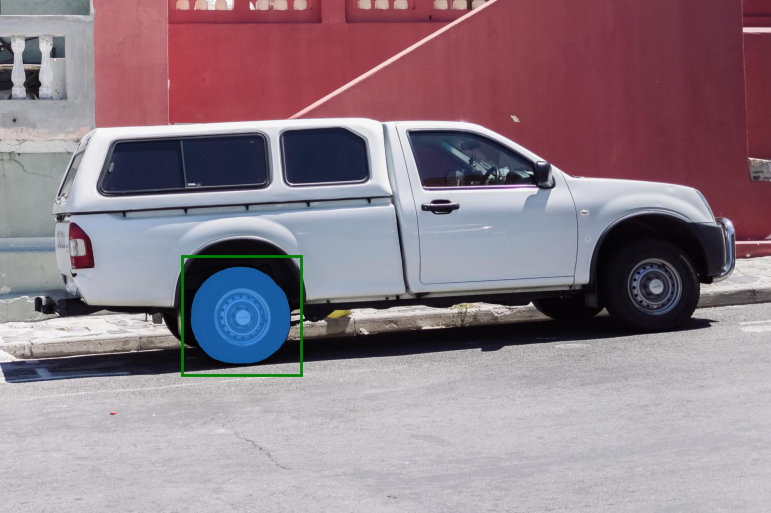
\includegraphics[width=\textwidth]{text/chapter_04/imgs/SAM_box}
    \caption{By defining an object by a bounding box, SAM is able to make a segmented masks of this object and choose
    the most probable one.}
    \label{fig:sam_box}
  \end{subfigure}
  \hfill
  \begin{subfigure}[h]{0.48\textwidth}
    \centering
    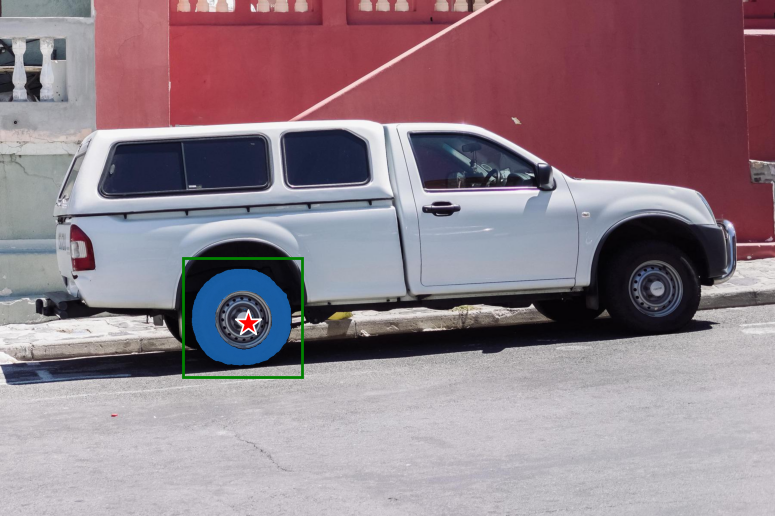
\includegraphics[width=\textwidth]{text/chapter_04/imgs/SAM_box_point}
    \caption{If we use a bounding box together with a point, we receive a different result. Here, just the trucks's
    tire, instead of the entire wheel, is selected.}
    \label{fig:sam_boxPoint}
  \end{subfigure}
  \caption{Comparison of using only a bounding box vs combination of a bounding box and a point as an input for SAM.}
  \label{fig:sam_examples}
\end{figure}

The combination of the SAM model with an object detector can segment an object with high precision and accuracy.
The cooperation of these two models is demonstrated in Figure \ref{fig:yolo_sam_seg}.
\begin{figure}[h!t]
  \centering
  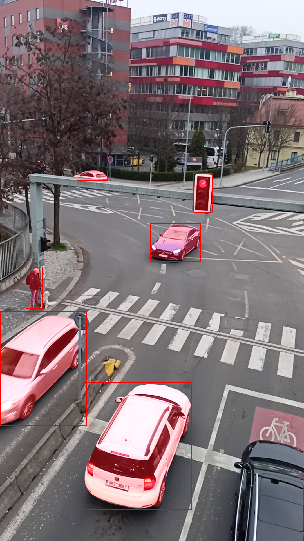
\includegraphics[width=0.35\linewidth]{text/chapter_04/imgs/YOLO_SAM_02}
  \caption{The cooperation of YOLO and SAM models. The YOLO provides bounding boxes of objects, which are inputs to
  SAM. The SAM model then makes segmented masks of these objects.}
  \label{fig:yolo_sam_seg}
\end{figure}

\subsection{S3: Grounded SAM + PHD}
Grounding DINO is an object detector that denotes objects in an image, based on a given text prompt. This feature
allows us to potentially track all the required objects without the need to fine tune every class instance to a model.
Moreover, this
model is able to mark objects based on an ambiguous text input. Despite this universality,
in cases where the
model is not confident enough that the desired object appears in a scene, different results can be received with
the same input every time the model is executed. This brings uncertainty in situations with ambiguous text inputs
and we should be aware of it in practical scenarios.

For a segmentation task, Grounding DINO's output serves as an input to the SAM model, as it produces bounding boxes
of the
detected objects.
SAM uses these bounding boxes to segment objects and creates segmentation binary masks. The cooperation of these models is demonstrated in Figure \ref{fig:GroundedSAM}.

\begin{figure}[h]
  \centering
  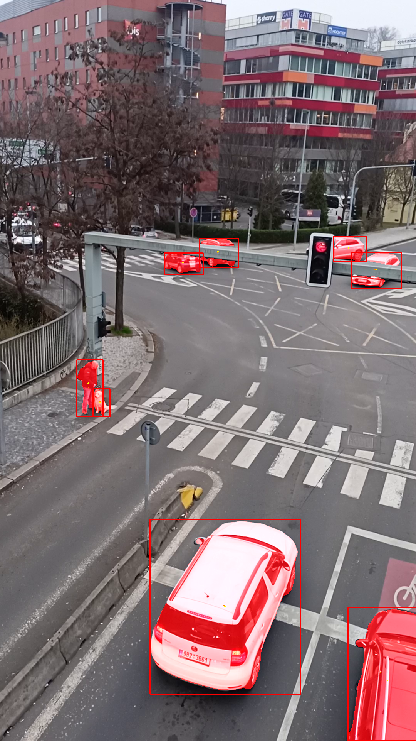
\includegraphics[width=0.35\linewidth]{text/chapter_04/imgs/DINO_example}
  \caption{The result of the Grounded SAM model. Grounding DINO marks objects with bounding boxes and SAM segments
  objects inside these bboxes. Marked objects are founded by Grounding DINO with text input \textit{person, car}.}
  \label{fig:GroundedSAM}
\end{figure}



\section{Dynamic detection probability in video data}
\label{sec:dynamic_pd}
To model the dynamic state- and time-dependent detection probability $p_{D,k}(x)$, we propose to base the current
point estimate of $p_{D}(x)$ at time $k$ on the similarity of the subsequent frame properties,

  \begin{align}
    p_{D,k}(x) &= \frac{\sum_{\sigma_j \in S_{sim}} \sum_{i=1}^{|H|}
      \sigma_j\left[h_i\left(M(x; k|k-1) \!\circ\! D_k\right),
        h_i\left(M(x; k-1) \!\circ\! D_k\right)\right]}{\|S_c\| \cdot \|H\|}, \label{eq:similarity}
  \end{align}

where $D_k$ is the frame in the given color spectrum, $h_i(\cdot)$ is a color histogram made from given color spectrum
, $A\circ B$ is the Hadamard product, $M(\cdot, \cdot)$ is the object binary mask, and $\sigma_j[\cdot, \cdot]$ is
the given similarity of two vectors. The $\|\cdot\|$ values in the denominator represent the set size. The whole
fraction is, in fact, the mean value across all color spectra and similarity functions.

There are many color spectra to consider, each providing certain benefits and downsides. The list of color spectra used
in this work is as follows.
\begin{itemize}
  \item \textbf{RGB} -- The RGB (Red, Green, Blue) color model is ubiquitous in electronic displays, digital cameras, and computer graphics. It defines colors by their intensities of red, green, and blue components. One of its
  primary advantages lies in its widespread use and an intuitive representation for additive color mixing. However,
  RGB lacks direct perceptual relevance to human vision, as it does not inherently represent attributes like brightness
  or hue.
  \item \textbf{XYZ} -- In contrast, the XYZ color space, established by the International Commission on Illumination
  (CIE), serves as a standard for quantifying colors in scientific and industrial applications. Even though it offers a
  device-independent color representation and facilitates color matching and conversion, it is not as perceptually
  intuitive and can be complex to work with practically.
  \item \textbf{HSV} -- HSV (Hue, Saturation, Value) is favored in graphics software and image editing for its
  intuitive representation of color. It aligns better with human perception compared to RGB, allowing independent
  adjustment of hue, saturation, and brightness. It lacks the widespread hardware and software support enjoyed by RGB
 and may not be as straightforward for certain color manipulation
  tasks.
  \item \textbf{LAB} -- LAB (CIELAB color space), another CIE-defined model. Unlike
  XYZ, it aims for perceptual uniformity. Widely used in color correction, image editing, and color management, LAB
  offers uniform changes in perceived color with uniform changes in LAB values. Despite its perceptual accuracy, it
  can be complex to comprehend and lacks universal software and hardware support compared to simpler models like RGB
  or HSV.
  \item \textbf{HLS} --  HLS (Hue, Lightness, Saturation) finds its place in computer graphics and image editing
  applications. Similar to HSV but with lightness instead of value, HLS provides an intuitive representation for
  color adjustment tasks. Unfortunatelly, its support may not be as widespread as RGB or HSV, and it may lack the
  perceptual accuracy of LAB in certain color correction scenarios.
\end{itemize}

We apply a range of similarity functions, each with its unique advantages and limitations. These functions include cosine similarity, intersection, and correlation.
\begin{itemize}
  \item \textbf{Cosine similarity} -- Cosine similarity, a widely used metric, determines the cosine of the angle
  between two vectors in a multi-dimensional space. It is insensitive to vector magnitudes, focusing more on their
  orientation, which proves valuable when the absolute magnitude of vectors is less crucial than their relative
  orientations. However, cosine similarity does not take into account the distribution of data points. Cosine
  similarity is defined as
  \begin{align}
    S_{cos} [A,B] &= \frac{A\cdot B}{\|A\|\|B\|} = \frac{\sum_{i=1}^nA_iB_i}{\sqrt{\sum_{i=1}^nA_i^2} \cdot \sqrt{\sum_{i
    =1}^n B_i^2}},
  \end{align}
  where the sums run over all elements of the arguments.
  \item \textbf{Intersection} -- Intersection similarity, on the other hand, calculates the overlap between two sets. This metric is commonly employed in applications like document retrieval and collaborative filtering. Its
  simplicity and intuitiveness make it ideal for comparing binary data or sets, where the presence or absence of
  elements is more significant than their values. Additionally, it treats all elements equally, disregarding their
  magnitudes, which can be a limitation in certain contexts. The intersection is formulated
    \begin{align}
      S_{inter}[A,B] &= \frac{\sum_{i=1}^{\|A\|} min(A_i, B_i) }{\sum_{i=1}^{\|B\|} B_i},
    \end{align}
    where $\|\cdot\|$ denotes the set size.
  \item \textbf{Pearson correlation coefficient} -- Correlation measures the linear relationship between two
  variables and is frequently used in statistics, finance, and signal processing. It captures both the strength and
  direction of the relationship between variables, making it valuable for identifying patterns and dependencies in
  data. Moreover, correlation assumes a linear relationship between variables, which may not always hold true, and it
  is susceptible to outliers and non-linear relationships, potentially  affecting its reliability in certain scenarios. In this work, we calculate the correlation between corresponding elements in sets $A, B$ as
    \begin{align}
      S_{corr}[A,B] &= \frac{cov(A,B)}{\sigma_A \sigma_B},
    \end{align}
    where $cov$ is the covariance and $\sigma_{(\cdot)}$ is the standard deviation,
\end{itemize}

For simplicity, let us denote the fraction in \eqref{eq:similarity} as $S_c$. This value represents the "average"
similarity across all used color spectra and similarity functions.

As mentioned in Section \ref{sec:mGMPHDrec}, the dynamically estimated detection probability in \eqref{eq:mphd_recursion_update_intesity} follows from one of two possible scenarios. First, there is no current measurement at
time $k$, hence the current mask results from its predicted position,
\begin{align}
  \label{eq:mphd_recursion_update_intesity_misdetect_pd}
  p_{D,k}^{(i)}(x) &=
  \begin{cases}
     S_c^{(i)}\left[h(M_{k|k-1}^{(i)}(x) \circ D_k), h_{0,k}^{(i)}\right] &\text{if $h_{0,k}^{(i)}$ exists,} \\
     p_{D,k}^{(i)} \quad& \text{otherwise,}
  \end{cases}
\end{align}
and where the histogram from the last detection $h_{0,k}^{(i)} \equiv  h_{0,k-1}^{(i)}$ is used in the first scenario. A user-preset value $p_{D,k}^{(i)}$ is used for targets undetected so far. The mask is obtained via
\begin{align}
  \label{eq:mphd_recursion_update_intesity_misdetect_M_shifted}
  M_{k|k-1}^{(i)}(x) &=
  \begin{cases}
    \!M_{k-1}^{(i)}(x)[m-v_x, n-v_y] &\text{if $m\geq v_x, n\geq v_y$,} \\
    \mathbf{0} \quad &\text{otherwise,}
  \end{cases}
\end{align}
where $m, n$ are indices of the binary mask $M$ and $v_x, v_y$ are x- and y-direction velocities of the target. $\mathbf{0}$ is a zero vector of the same size as the mask. The second scenario takes the current measurement $z$ into account. The detection probability is modified according to
\begin{align}
  p_{D,k}^{(j)}(x;z) &= S_c\left[h(M_{k}^{(j)}(z) \circ D_k), h_{0,k}^{(j)}\right], \label{eq:mphd_recursion_update_intesity_misdetect_z_pd}
\end{align}
where $h_{0,k}^{(j)}$ is the histogram resulting from the last detection,
\begin{equation}
  \label{eq:mphd_recursion_update_intesity_misdetect_Hist}
  h_{0,k}^{(j)} =
  \begin{cases}
    h(M_{k-1}^{(j)}(z) \circ D_{k-1}) &\text{if } h(M_{k-1}^{(j)}(z)) \text{ exists,} \\
    % h(M_{k|k-1}^{(j)}(x) \circ D_{k_0}) &\text{otherwise,} \\
    h_{0,k-1} &\text{otherwise.}
  \end{cases}
\end{equation}
The histogram $h(M_{k-1}^{(j)}(z) \circ D_{k-1})$ stands for the previously detected target, and $h_{0,k-1}$ is the histogram from the time step when the target was detected the last time.



\section{Modified pruning for GM-PHD filter}
As the PHD filter propagates the posterior intensity, the number of potential hypotheses exponentially increases.
This leads to an enormous increase in memory and computational demands. Pruning techniques become indispensable in
mitigating this computational load by selectively discarding less likely hypotheses, allowing for a more focused and
efficient tracking process. These pruning mechanisms, guided by predefined thresholds or heuristics, ensure that the
computational resources are allocated judiciously, striking a balance between accuracy and computational efficiency in multi-target tracking applications.

Recall that sensors in our work are represented by cameras. Naturally, the detecting algorithms are unable to
recognize an object hidden by an obstacle. These obstacles may differ not only in size but also in color. In
situations where the color of an obstacle closely matches the surrounding scene, the likelihood of detection remains
sufficiently high, increasing the risk that the target may not survive even though it is only hidden. In order to suppress this phenomenon, we introduce a method for modified pruning along with standard pruning and merging techniques \cite{VoMaPHD2006}.

The most deployed generic method for pruning consists of removing targets with weights below some predefined threshold. Nonetheless, as mentioned before, targets with some history may only be hidden, and it is not desired to remove these targets from the scene. To overcome this issue, we assign each target a tag that represents the state in which the target is likely to occur,
\begin{equation}
  S = \{\text{detected, hidden, dead}\}.
  \notag
\end{equation}
This tag is modeled by a discrete-time Markov chain with the transition matrix
\begin{align}
  \label{eq:mphd_transition_matrix}
  P &= \begin{bmatrix}
         p_{D,k} & 1-p_{D,k} & 0 \\
         p_{D,k} & (1-p_{H,k}^{T_H}) \cdot (1-p_{D,k}) & p_{H,k}^{T_H} \cdot (1- p_{D,k}) \\
         p_{D,k} & (1-p_{H,k}^{T_H}) \cdot (1-p_{D,k}) & p_{H,k}^{T_H} \cdot (1- p_{D,k})
  \end{bmatrix},
\end{align}
where $p_{D,k}$ is a generic detection probability, and $T_H$ is an exponent for controlling probabilities that is
set higher in scenarios, where the target color mask is similar to the color mask of the obstacle, or may be set
lower otherwise. $p_{H,k}$ is the probability that the target is removed. This probability is the result of \eqref{eq:mphd_recursion_update_intesity_misdetect_pH}, where the bounding boxes of the object detector are used.
If we denote by $B_{P,k}^{(j)}$ the bounding box predicted $T_c$ steps ahead and by $B_{S,k}^{(j)}$ the bounding box of the last step $k$ when the object was detected, then
\begin{align}
  B_{P,k}^{(j)} &= B_{P,k-1}^{(j)} + n_k^{(j)}\cdot [v_{x,{k}}^{(j)}, v_{y,{k}}^{(j)}, _{x,{k}}^{(j)}, v_{y,{k}}^{(j)}], \label{eq:mphd_bbox_shift}\\
  B_{S,k}^{(j)} &= B_{S,k-1}^{(j)}, \\
  p_{H,k} &= S_c\left[D_k(B_{P,k}^{(j)}), D_k(B_{S,k}^{(j)})\right], \label{eq:mphd_recursion_update_intesity_misdetect_pH}
\end{align}
where
\begin{align}
  \label{eq:mphd_recursion_update_intesity_misdetect_T_move}
  n_k^{(j)} &=
  \begin{cases}
    T_c \quad & \text{if } k\text{ } mod \text{ }T_c = 0,  \\
    0 \quad & \text{otherwise.}
  \end{cases}
\end{align}
$D_k(\cdot)$ is a part of a frame within the bounding box given by $B(\cdot)$. With this approach, when a target is most likely in the \textit{hidden} state, the pruning threshold is heuristically lowered to prevent the target removal.

In summary, first we define a birth place in a scene. We call this birth place a spawn point (SP). It is possible to
define more spawn points in a scene, depending on the situation. If a target crosses this spawn point, it is
initialized, and since it is the first time the target has been seen, the detection probability is a predefined
constant. In the
next time step, suppose that the target is detected and there is one measurement (originating from this target) in the
validation region. Due to the GM-PHD recursion, two new targets arise from the previous target with the state $\xi$.
One originates from
the misdetection possibility and one from the measurement. As
we first predict the target's position and covariance
matrix, we move the target's mask detected at time $k-1$ to $k$ by its velocity (in case of the CVM model). Then the
predicted mask color properties are compared to the mask made from the new measurement from time $k$. If nothing
unpredictable happens, both masks should occur on a very similar position, thus the color masks' properties should be
very similar. It such case, the detection probability is very likely to be high, lowering the weight of the
misdetection-born target. As the weight is small, the target is likely to be removed during the pruning step.

If the previously detected target is hidden behind an obstacle and the object detector does not provide any
measurement, only misdetection-born target arises. In such case, the mask from the time when the target was lastly
detected is compared to the predicted mask that now also contains the obstacle's color properties. Due to using
cameras as
a sensor, frames at high frame rate are produced. It is not desired to lower fps to something like 1 fps, as a lot of
information are lost. We lower the fps to 10-20 fps to enhance the dynamics of the scene. However, in a such short time
period, the target, e.g. a car, does not move enough. The predicted mask then intersects with the lastly
detected target's mask by a considerably huge amount. That is why we define a hidden probability $p_{H,k}$ and modify
the pruning of components. As the masks are likely to intersect, the detection probability is likely to be high in
the first couple of frames, where the target is hidden. It is essential for the target to survive through this time
period. The hidden probability is based on the color properties of bounding boxes from the time the target was lastly
detected
and from the bounding box that is moved $T_c$ time steps ahead in the direction of the target's velocity. The moved
bounding box reveals the color properties of the obstacle, that are likely to be different from those assigned to the
target
when it was lastly detected. Then, the hidden probability should be low and the target's state should be in a hidden
state,
based on \ref{eq:mphd_transition_matrix}, therefore the pruning threshold is lowered. After the target overtakes the
obstacle,
it should appear in a scene and be detected again. If it does not and the color properties of a scene given by the
moving
bounding box differ from the ones captured when the target was lastly detected, the hidden probability is high and the
target is
in a dead state. The pruning threshold is not lowered and the detection probability is low, so the target is removed
during the pruning step.
\section{Merging in GM-PHD filter with dynamic detection probability}
Another way to lower the computational demands and to potentially increase the robustness of a filter is through
merging of the
targets that appear in the same neighbourhood. This procedure is especially useful in situations when many measurements
occur in a validation region of a target. If at least some of these measurements originate from clutter, the target
count increases rapidly due to the
GM-PHD recursion, increasing the computational requirements. To prevent this issue,
the target merging technique is necessary.
In the GM-PHD filter, each target carries three variables: the target's weight $w$, mean $m$ and a covariance matrix $P$.
Merging these values of multiple filters is straightforward and is described in \cite{VoMaPHD2006} and Section \ref{sec:phd_pruning_and_merging}. However, in our modified GM-PHD filter, each target also holds these information:
\begin{itemize}
  \item \textbf{Current bounding box position:} The bbox in $xyxy$ format determines current position of an object.
  This bbox is determined by a bbox given by a measurement $z$ in the current time step $k$ in an update step. The
  target's
  bbox is shifted in the prediction step in \eqref{eq:mphd_bbox_shift}, thus the target must have been initialized in
  the
  past in order to have the current bbox.
  \item \textbf{Current mask:} The current binary mask is given by a measurement $z$ in the current time step $k$ in
  the update
  step. In order to inialize current mask, it must have been initialized by a measurement in
  the past. The mask is shifted according to \eqref{eq:mphd_recursion_update_intesity_misdetect_M_shifted}.
  \item Data structure \textbf{Object Stats:} Every new target born in the update step of the GM-PHD filter by a
  measurement $z$ from a target with a previous state $\xi$, contains a data structure \textit{Object Statss}. This
  structure is composed of many variables determining the target's history. These variable arise in the update step from
  a measurement and are useful for calculating the dynamic detection probability in Equations
  \eqref{eq:mphd_recursion_update_intesity_misdetect_pd} - \eqref{eq:mphd_recursion_update_intesity_misdetect_pH}.
      \begin{itemize}
        \item \textbf{Bounding box position:} This variable in Object stats represents a bounding box from the time
        the target was lastly detected. To calculate $p_{H,k}$ in
        \eqref{eq:mphd_recursion_update_intesity_misdetect_pH}, this and the current bbox are compared.
        \item \textbf{Mask:} This variable represents the target's mask from the time the target was lastly detected. In \eqref{eq:mphd_recursion_update_intesity_misdetect_pd} and \eqref{eq:mphd_recursion_update_intesity_misdetect_z_pd} this mask is compared to the current mask
        resulting from the prediction step of a target with the previous state $\xi$.
        \item \textbf{Frame:} To compare the color histograms in \eqref{eq:mphd_recursion_update_intesity_misdetect_pd}
        and \eqref{eq:mphd_recursion_update_intesity_misdetect_z_pd}, each target contains a frame from the time $k$
        in which
        it was born.
        \item \textbf{Time stamp:} This is a variable to save the time $k$ the target was born.
      \end{itemize}
  \item Data structure \textbf{Markov Chain:} This data structure determines the target's state. As the
  distribution determined by a transition matrix in \eqref{eq:mphd_transition_matrix} is not stationary, it is necessary
  to calculate the resulting distribution in every time step.
      \begin{itemize}
        \item \textbf{Initial distribution:} To get the target's state, an initial distribution needs to be defined
        first.
        \item \textbf{Result matrix:} The result matrix is an ongoing outcome of a previous result matrix and a
        transition
        matrix, i.e, result matrix $R_k = R_{k-1} P^{k-k_0}$, where $k_0$ is the time the target was born,
        $R_0 = I_3$ and $I_n$ is the identity matrix of the shape $n\times n$.
      \end{itemize}
\end{itemize}

The merging procedure of the previous information is inspired by the original GM-PHD merging procedure in
\cite{VoMaPHD2006}.

The current bounding box merging is straightforward as $(x_1,y_1)$ and $(x_2,y_2)$ coordinates defining the bbox are
averaged using the targets' weight. Let us define a set $L$, which represents a subset of targets to merge into a single
target. Then a resulting target's bbox
\begin{align}
  \tilde{B}_k^{(l)} &= \frac{\sum_{i \in L} B_k^{(i)} * w_k^{(i)}}{\sum_{i \in L}{w_k^{(i)}}},
\end{align}
where $w_k^{(i)}$, is the weight of a target $i$ is the weighted mean of targets in subset $L$. The same procedure is
applied to the bounding box in \textit{Object Stats}, i.e., the previous bbox.

The merging of masks is slightly complicated, as we merge targets' masks into a single "average" mask. First, binary
masks of targets in the subset $L$ are converted into \textit{float} data type, then multiplied with targets' weight
and
divided by the sum of these weights. To get the resulting binary mask, each element of mask
\begin{align}
  \tilde{M}_k^{(l)} &= \frac{\sum_{i \in L} M_k^{(i)} * w_k^{(i)}}{\sum_{i \in L}{w_k^{(i)}}}
\end{align}
is rounded either to zero or one and the mask is converted to the binary data type.

We have not experimented with complicated merging of frames and time stamps, only argument maxima is used for both
values, i.e,
\begin{align}
  \tilde{t}_k^{(l)} &= max_{i \in L} t_k^{(i)}, \\
  \tilde{D}_k^{(l)} &= D_k^{(\tilde{t}_k^{(l)})}.
\end{align}

As the initial distribution is the same for every target, the resulting merged target's initial distribution is only a
copy of any target in $L$.

The result matrix merging procedure is similar to the bounding box distribution. The result matrix
\begin{align}
  \tilde{N}_k^{(l)} &= \frac{\sum_{i \in L} N_k^{(i)} * w_k^{(i)}}{\sum_{i \in L}{w_k^{(i)}}}
\end{align}
is the "average" result matrix of targets in subset $L$.

The pseudo-code algorithm of modified pruning in GM-PHD filter is shown in Algorithm \ref{alg:mphd_merging}.
\begin{algorithm}
  \caption{Pseudo-algorithm for pruning in the GM-PHD filter}
  \begin{algorithmic}[1]
    \Require{$\{w_{k}^{(i)}, m_{k}^{(i)},P_{k}^{(i)}, B_{k}^{(i)}, M_{k}^{(i)}, B_{OS,k}^{(i)}, M_{OS,k}^{(i)}, t_{OS
    ,k}^{(i)}, D_{k}^{(i)}, G_{OS,k}^{(i)}, N_{OS,k}^{(i)}\}_{i=
    1}^{J_{k}}$, a
    truncation
    threshold T, a
    merging
    threshold U and a maximum number of allowed Gaussian terms $J_{max}$. Set $l=0,$ and
      $I = \{ i=1,\dots, J_k | w_k^{(i)} > T\}$.}
    \Procedure{Merging of targets}{}
      \While{$I \neq \emptyset$}
        \State $l:= l+1$
        \State $j:= \text{argmax}_{i \in I} w_k{(i)},$
        \State $L:= \left\{ i \in I | (m_k^{(i)} - m_k^{(j)})^T (P_k{(i)})^{-1} (m_k^{(i)} - m_k^{(j)}) \leq U \right\},$
        \State $\tilde{w}_k^{(l)} = \sum_{i \in L} w_k^{(i)}$,
        \State $\tilde{m}_k^{(l)} = \frac{1}{\tilde{w}_k^{(l)}} \sum_{i \in L} w_k{(i)} x_k^{(i)},$
        \State $\tilde{P}_k^{(l)} = \frac{1}{\tilde{w}_k^{(l)}} \sum_{i \in L} w_k^{(i)} (P_k^{(i)} + (m_k^{(l)} - m _k^{(i)}) (m_k^{(l)} - m _k^{(i)})^T,$
        \State $\tilde{B}_k^{(l)} = \frac{1}{\tilde{w}_k^{(l)}} \sum_{i \in L} B_k^{(i)} * w_k^{(i)}$
        \State $\tilde{M}_k^{(l)} = round(\frac{1}{\tilde{w}_k^{(l)}} \sum_{i \in L} M_k^{(i)} * w_k^{(i)})$
        \State $\tilde{B}_{OS,k}^{(l)} = \frac{1}{\tilde{w}_k^{(l)}} \sum_{i \in L} B_{OS,k}^{(i)} * w_k^{(i)}$ \Comment{OS stands for Object Stats}
        \State $\tilde{M}_{OS,k}^{(l)} = round(\frac{1}{\tilde{w}_k^{(l)}} \sum_{i \in L} M_{OS,k}^{(i)} * w_k^{(i)})$
        \State $\tilde{t}_{OS,k}^{(l)} = max_{i \in L} t_{OS,k}^{(i)}$
        \State $\tilde{D}_{OS,k}^{(l)} = D_k^{(\tilde{t}_{OS,k}^{(l)})}$
        \State $\tilde{G}_{OS,k}^{(l)} = {G}_{OS,k}^{(j)}$ \Comment{Initial distribution of Markov process}
        \State $\tilde{N}_{OS,k}^{(l)} = \frac{1}{\tilde{w}_k^{(l)}} \sum_{i \in L} N_{OS,k}^{(i)} * w_k^{(i)}$
        \State $I:= I/L.$
      \EndWhile
    \EndProcedure
    \State
    \State If $l > J_{max}$ then replace $\{ \tilde{w}_k^{(i)}, \tilde{m}_k^{(i)}, \tilde{P}_k^{(i)}, \tilde{B}_k^{(i
    )}, \tilde{M}_k^{(i)}, \tilde{B}_{OS,k}^{(i)}, \tilde{M}_{OS,k}^{(i)}, \tilde{t}_{OS,k}^{(i)}, \tilde{D}_{OS,k}^{(i)}, \tilde{G}_{OS,k}^{(i)}, \tilde{N}_{OS,k}^{(i)} \}_{i=1}^l$ by
    those of the $J_{max}$ Gaussians with largest weights.
    \State
    \State Output: $\{ \tilde{w}_k^{(i)}, \tilde{m}_k^{(i)}, \tilde{P}_k^{(i)}, \tilde{B}_k^{(i
    )}, \tilde{M}_k^{(i)}, \tilde{B}_{OS,k}^{(i)}, \tilde{M}_{OS,k}^{(i)}, \tilde{t}_{OS,k}^{(i)}, \tilde{D}_{OS,k}^{(i)}, \tilde{G}_{OS,k}^{(i)}, \tilde{N}_{OS,k}^{(i)} \}_{i=1}^l$ as pruned Gaussian components.

  \end{algorithmic}
  \label{alg:mphd_merging}
\end{algorithm}

\chapter{Experiments}

\appendix\appendixinit % do not remove these two commands



\chapter{Nějaká příloha}


Sem přijde to, co nepatří do hlavní části.
 % include `appendix.tex' from `text/' subdirectory



\backmatter % do not remove this command

\printbibliography % print out the BibLaTeX-generated bibliography list

\chapter{Gitlab repository}
% Concents of the attachment
All source codes for the practical part of this thesis and text files in \LaTeX{} form can be found in author's 
faculty gitlab repository here: \href{https://gitlab.fit.cvut.cz/seibemic/dp/-/tree/master/src?ref_type=heads}
{gitlab.fit.cvut.cz/seibemic/dp}.

\vspace{2cm}
	\dirtree{%
		.1 README.md \DTcomment{Brief introduction to this thesis}.
		.1 src \DTcomment{Source files of this thesis}.
		.2 experiments \DTcomment{Figures and graphs for experiments}.
		.2 impl \DTcomment{Source code of the implementation of the proposed method}.
		.3 PHD.ipynb \DTcomment{Jupyter notebook dedicated for trying out the method}.
		.2 text \DTcomment{Folder including files for this thesis in \LaTeX{} form}.
		.1 seibemic-thesis.pdf \DTcomment{The text of this work in PDF format}.
	}
 % include `medium.tex' from `text/' subdirectory

\end{document}
